% ====================================================================
% TCC - Sistema de Assinatura Eletrônica via Link com Registro Imutável
% em Blockchain utilizando Smart Contracts
% Classe: abnTeX2 (padrão ABNT para trabalhos acadêmicos brasileiros)
% ====================================================================
\documentclass[
    12pt,
    a4paper,
    oneside,
    chapter=TITLE,
    section=TITLE,
    subsection=TITLE,
    subsubsection=TITLE,
    sumario=tradicional,
    english,
    brazil
]{abntex2}

% ---------------------------------------------------------------
% Pacotes
% ---------------------------------------------------------------
\usepackage[utf8]{inputenc}
\usepackage[T1]{fontenc}
\usepackage{lmodern}
\usepackage[brazil]{babel}
\usepackage{indentfirst}
\usepackage{color}
\usepackage{graphicx}
% Página em modo paisagem (usada no diagrama de sequência), já girada no leitor de PDF.
\usepackage{pdflscape}
\usepackage{microtype}
\usepackage{booktabs}
\usepackage{longtable}
\usepackage{array}
% Coluna de largura fixa com texto alinhado à esquerda (usada nos quadros).
\newcolumntype{L}[1]{>{\raggedright\arraybackslash}p{#1}}
\usepackage{hyperref}
\usepackage[brazilian,hyperpageref]{backref}
\usepackage[alf]{abntex2cite}
\usepackage{placeins}
% ---- Listagens de código e de saídas de programas (usadas nos apêndices) ----
\usepackage{listings}
\usepackage{pifont}
\lstdefinelanguage{Solidity}{
    morekeywords={pragma, solidity, contract, struct, mapping, address,
        public, private, immutable, external, view, event, error,
        constructor, function, returns, return, if, revert, emit, memory,
        indexed, bytes32, uint64, uint256, bool},
    sensitive=true,
    morecomment=[l]{//},
    morecomment=[s]{/*}{*/},
    morestring=[b]",
}
\lstset{
    basicstyle=\ttfamily\footnotesize,
    columns=flexible,
    keepspaces=true,
    breaklines=true,
    breakatwhitespace=true,
    postbreak=\mbox{$\hookrightarrow$\space},
    showstringspaces=false,
    tabsize=4,
    frame=single,
    framesep=4pt,
    rulecolor=\color[gray]{0.6},
    aboveskip=6pt,
    belowskip=6pt,
    extendedchars=true,
    literate=
        {á}{{\'a}}1 {à}{{\`a}}1 {â}{{\^a}}1 {ã}{{\~a}}1
        {é}{{\'e}}1 {ê}{{\^e}}1 {í}{{\'i}}1 {ó}{{\'o}}1
        {ô}{{\^o}}1 {õ}{{\~o}}1 {ú}{{\'u}}1 {ç}{{\c{c}}}1
        {Á}{{\'A}}1 {É}{{\'E}}1 {Í}{{\'I}}1 {Ó}{{\'O}}1
        {Ú}{{\'U}}1 {Ç}{{\c{C}}}1
        {✔}{{\ding{52}}}1 {ℹ}{{\textbf{i}}}1
}
% Código-fonte: palavras-chave em negrito, comentários em itálico e linhas numeradas.
\lstdefinestyle{codigo}{
    language=Solidity,
    keywordstyle=\bfseries,
    commentstyle=\itshape\color[gray]{0.35},
    numbers=left,
    numberstyle=\tiny\color[gray]{0.4},
    numbersep=8pt,
    xleftmargin=2em,
}
% Saída de programas: texto como impresso no terminal, sem numeração.
\lstdefinestyle{saida}{
    numbers=none,
}
% ---- Destaque para elementos dos diagramas UML (classes, relações, atores, estados) ----
\newcommand{\elem}[1]{\texttt{#1}}
% Nomes em fonte monoespaçada não são hifenizados; folga extra evita linhas além da margem
\setlength{\emergencystretch}{2em}


% ---- Ambiente "quadro" (não é definido por padrão no abnTeX2) ----
\newcommand{\quadroname}{Quadro}
\newcommand{\listofquadrosname}{Lista de quadros}
\newfloat[chapter]{quadro}{loq}{\quadroname}
\newlistof{listofquadros}{loq}{\listofquadrosname}
\newlistentry{quadro}{loq}{0}
\setfloatadjustment{quadro}{\centering}
\counterwithout{quadro}{chapter}
\renewcommand{\cftquadroname}{\quadroname\space}
\renewcommand*{\cftquadroaftersnum}{\hfill--\hfill}
% Posição [H] (fixa no ponto do texto), usada no dicionário de dados; carregado
% depois do \newfloat acima, pois antes dele entra em conflito com o memoir.
\usepackage{float}

% Páginas compostas só por figuras ou quadros começam no topo, sem
% centralização vertical.
\makeatletter
\setlength{\@fptop}{0pt}
\setlength{\@fpbot}{0pt plus 1fil}
\makeatother

% ---------------------------------------------------------------
% Configurações de hyperref / backref (padrão abnTeX2)
% ---------------------------------------------------------------
\hypersetup{
    pdftitle={Sistema de Assinatura Eletrônica via Link com Registro Imutável em Blockchain utilizando Smart Contracts},
    pdfauthor={Vinícius Fosquiera Teigão},
    pdfsubject={Trabalho de Conclusão de Curso},
    pdfkeywords={blockchain, smart contracts, assinatura eletrônica, Ethereum, PKI},
    colorlinks=true,
    linkcolor=black,
    citecolor=black,
    filecolor=black,
    urlcolor=blue,
    bookmarksdepth=4
}

\renewcommand{\backrefpagesname}{Citado na(s) página(s):}
\renewcommand{\backref}{}
\renewcommand*{\backrefalt}[4]{
    \ifcase #1
        Nenhuma citação no texto.
    \or
        Citado na página #2.
    \else
        Citado nas páginas #2.
    \fi
}

% ---------------------------------------------------------------
% Dados do trabalho
% ---------------------------------------------------------------
\titulo{Sistema de Assinatura Eletrônica via Link com Registro Imutável em Blockchain utilizando Smart Contracts}
\autor{Vinícius Fosquiera Teigão}
\local{Foz do Iguaçu, PR}
\data{2026}
\instituicao{%
    Centro Universitário Dinâmica das Cataratas
    \par
    Curso de Bacharelado em Ciência da Computação
}
\tipotrabalho{Trabalho de Conclusão de Curso}
\preambulo{%
    Projeto da Disciplina de Projeto de Graduação II do Curso de
    Bacharelado em Ciência da Computação, apresentado à UDC como
    requisito parcial para obtenção do título de bacharel em Ciência da
    Computação.
    \par\medskip
    \textbf{Orientador}: Prof. Dr. Miguel Diogenes Matrakas
}
\orientador{Prof. Dr. Miguel Diogenes Matrakas}

% ---------------------------------------------------------------
% Configurações de aparência do PDF
% ---------------------------------------------------------------
\makeatletter
\hypersetup{
     pdftitle={\@title},
     pdfauthor={\@author}
}
\makeatother

\setlength{\parindent}{1.3cm}
\setlength{\parskip}{0.2cm}

% ---------------------------------------------------------------
% compila o índice
% ---------------------------------------------------------------
\makeindex

% ---------------------------------------------------------------
% Início do documento
% ---------------------------------------------------------------
\begin{document}

% Espaçamento entre linhas e parágrafos
\SingleSpacing

% ---------------------------------------------------------------
% ELEMENTOS PRÉ-TEXTUAIS
% ---------------------------------------------------------------
\pretextual

% ---- Capa ----
\imprimircapa

% ---- Folha de rosto ----
\imprimirfolhaderosto

% ---- Dedicatória (NBR 14724: sem título, antes dos agradecimentos) ----
\begin{dedicatoria}
    \vspace*{\fill}
    \begin{flushright}
        \begin{minipage}{0.5\textwidth}
            \itshape\raggedright
            Dedico este trabalho aos meus pais, que, com amor e sacrifício, nunca mediram esforços para que eu pudesse estudar e sempre acreditaram em mim. Sem o apoio, os ensinamentos e a presença constante deles, esta conquista não teria sido possível. A~vocês, toda a minha gratidão.
        \end{minipage}
    \end{flushright}
\end{dedicatoria}

% ---- Agradecimentos (NBR 14724: antes do resumo) ----
\begin{agradecimentos}
Agradeço, primeiramente, a Deus, pela vida, pela saúde e pela força que me sustentaram ao longo desta caminhada e me permitiram superar as dificuldades até a conclusão deste trabalho.

Aos meus pais, pelo amor, pelo apoio incondicional e pelos esforços dedicados à minha formação. Sem o incentivo e o exemplo que sempre me deram, esta conquista não seria possível.

À minha namorada, pelo carinho, pela paciência e pela compreensão nos momentos em que precisei me dedicar a este trabalho, e por estar ao meu lado em todas as etapas desta jornada.

Aos meus amigos, pelo companheirismo, pelas palavras de incentivo e pelos momentos de descontração, que tornaram este percurso mais leve.

Ao meu orientador, Prof. Dr. Miguel Diogenes Matrakas, pela orientação, pela disponibilidade e pelas contribuições que aprimoraram este trabalho.
\end{agradecimentos}

% ---- Epígrafe (NBR 14724: depois dos agradecimentos, antes do resumo) ----
\begin{epigrafe}
    \vspace*{\fill}
    \begin{flushright}
        \begin{minipage}{0.5\textwidth}
            \raggedright
            \textit{``Por mais difícil que a vida possa parecer, sempre há algo que você pode fazer e ter sucesso. O~importante é não desistir.''}
            \par\medskip
            \raggedleft
            Stephen Hawking
        \end{minipage}
    \end{flushright}
\end{epigrafe}

% ---- Resumo na língua vernácula ----
\setlength{\absparsep}{18pt}
\begin{resumo}
A coleta remota de assinaturas em documentos ainda enfrenta obstáculos, e as soluções de registro em \emph{blockchain} costumam exigir que o signatário possua carteira digital e compreenda o pagamento de taxas de transação. Este trabalho desenvolve um sistema de assinatura eletrônica via link com registro imutável na \emph{blockchain} Ethereum por meio de contrato inteligente, acessível a usuários sem conhecimento técnico, com foco inicial no Documento de Formalização da Demanda (DFD), instrumento das contratações públicas. A pesquisa, de natureza aplicada e abordagem qualitativa com elementos quantitativos exploratórios, adota o desenvolvimento experimental em incrementos, apoiado na especificação de requisitos, na modelagem UML e na modelagem do banco de dados. O protótipo reúne um \emph{backend} em Node.js e Express, um banco de dados MySQL, páginas \emph{web} e um contrato inteligente em Solidity implantado na rede de testes Sepolia. No fluxo proposto, o remetente envia o documento em PDF, posiciona a caixa de assinatura e obtém um link único; o signatário confirma a identidade por CPF e data de nascimento, em até três tentativas, visualiza o documento e decide entre assinar e recusar. Na assinatura, o sistema confere o \emph{hash} SHA-256 do documento, coleta as evidências do ato e gera uma cópia com a caixa preenchida, sem alterar o original; em seguida, a carteira da plataforma assina e paga a transação que registra no contrato o \emph{hash} do documento e o \emph{hash} das evidências, sem enviar dados pessoais à rede. Os resultados mostram 37 testes automatizados aprovados e 60 fluxos completos, com até 25 signatários simultâneos, concluídos sem erro, com resposta máxima do \emph{backend} de 302 ms e todos os registros confirmados na primeira tentativa, em tempo mediano de 10,0 s. O contrato recusou o registro repetido de um documento e o registro feito por outra conta, a consulta pública funcionou sem custo e uma assinatura feita por outra pessoa, em outro computador e em outra rede, foi registrada normalmente. O teste de carga revelou um impasse no banco de dados, que foi corrigido. O custo estimado de um registro na rede principal ficou entre R\$~0,09 e R\$~0,29 com o preço mediano cobrado pela rede, conforme as regras de cobrança consideradas, valor pago pela plataforma, enquanto a fila de registro limitou a vazão a cerca de quatro registros por minuto. O signatário conclui a assinatura em três telas, sem carteira digital, criptomoeda ou instalação de software. Conclui-se que a proposta é tecnicamente viável quando a complexidade da \emph{blockchain} fica a cargo da plataforma, e que o sistema produz evidências de integridade e de autoria utilizáveis como meio de prova, sem substituir a assinatura qualificada baseada em certificado ICP-Brasil.

\textbf{Palavras-chave}: assinatura eletrônica; \emph{blockchain}; contratos inteligentes; Ethereum; integridade documental.
\end{resumo}

% ---- Resumo em língua estrangeira ----
\begin{resumo}[Abstract]
\begin{otherlanguage*}{english}
Remote collection of signatures on documents still faces obstacles, and blockchain-based registration solutions usually require the signer to own a digital wallet and to understand the payment of transaction fees. This work develops a link-based electronic signature system with immutable registration on the Ethereum blockchain through a smart contract, accessible to users without technical knowledge and initially focused on the Demand Formalization Document (\emph{Documento de Formalização da Demanda}, DFD), an instrument of Brazilian public procurement. The research is applied, with a qualitative approach and exploratory quantitative elements, and follows an incremental experimental development supported by requirements specification, UML modeling and database modeling. The prototype combines a Node.js and Express backend, a MySQL database, web pages and a Solidity smart contract deployed on the Sepolia test network. In the proposed flow, the sender uploads the PDF document, places the signature box and obtains a unique link; the signer confirms their identity with their CPF, the Brazilian individual taxpayer number, and their date of birth, within three attempts, views the document and chooses to sign or to decline. Upon signature, the system checks the SHA-256 hash of the document, collects the evidence of the act and generates a copy with the signature box filled in, leaving the original unchanged; the platform wallet then signs and pays for the transaction that records the document hash and the evidence hash in the contract, without sending personal data to the network. The results show 37 automated tests passed and 60 complete flows, with up to 25 simultaneous signers, completed without errors, with a maximum backend response time of 302 ms and all records confirmed on the first attempt, with a median confirmation time of 10.0 s. The contract rejected a repeated registration of the same document and a registration attempted by another account, the public query worked at no cost, and a signature made by another person, on another computer and another network, was recorded normally. The load test revealed a database deadlock, which was fixed. The estimated cost of one record on the main network ranged from BRL~0.09 to BRL~0.29 at the median network price, depending on the fee rules considered, and is paid by the platform, while the registration queue limited throughput to about four records per minute. The signer completes the signature in three screens, without a digital wallet, cryptocurrency or software installation. The work concludes that the proposal is technically feasible when the complexity of the blockchain is handled by the platform, and that the system produces evidence of integrity and authorship that can be presented as means of proof, without replacing the qualified signature based on an ICP-Brasil certificate.

\textbf{Keywords}: electronic signature; blockchain; smart contracts; Ethereum; document integrity.
\end{otherlanguage*}
\end{resumo}

% ---- Lista de figuras ----
\pdfbookmark[0]{\listfigurename}{lof}
\listoffigures*
\cleardoublepage

% ---- Lista de quadros ----
\pdfbookmark[0]{\listofquadrosname}{loq}
\listofquadros*
\cleardoublepage

% ---- Lista de abreviaturas e siglas ----
\begin{siglas}
    \item[DFD] Documento de Formalização da Demanda
    \item[PKI] Public Key Infrastructure (Infraestrutura de Chaves Públicas)
    \item[ICP-Brasil] Infraestrutura de Chaves Públicas Brasileira
    \item[EVM] Ethereum Virtual Machine
    \item[ECDSA] Elliptic Curve Digital Signature Algorithm
    \item[RSA] Rivest--Shamir--Adleman
    \item[EdDSA] Edwards-curve Digital Signature Algorithm
    \item[AC] Autoridade Certificadora
    \item[AR] Autoridade de Registro
    \item[CRL] Certificate Revocation List (Lista de Certificados Revogados)
    \item[OCSP] Online Certificate Status Protocol
    \item[DApp] Decentralized Application (Aplicação Descentralizada)
    \item[UML] Unified Modeling Language
    \item[MER] Modelo Entidade-Relacionamento
    \item[RF] Requisito Funcional
    \item[RNF] Requisito Não Funcional
    \item[AES] Advanced Encryption Standard
    \item[API] Application Programming Interface (Interface de Programação de Aplicações)
    \item[CPF] Cadastro de Pessoas Físicas
    \item[CSS] Cascading Style Sheets
    \item[GCM] Galois/Counter Mode
    \item[HTML] HyperText Markup Language
    \item[IDE] Integrated Development Environment (Ambiente de Desenvolvimento Integrado)
    \item[IP] Internet Protocol
    \item[JSON] JavaScript Object Notation
    \item[PDF] Portable Document Format
    \item[QR] Quick Response
    \item[RPC] Remote Procedure Call (Chamada de Procedimento Remoto)
    \item[SHA] Secure Hash Algorithm
    \item[SMS] Short Message Service (Serviço de Mensagens Curtas)
    \item[PK] Primary Key (Chave Primária)
    \item[FK] Foreign Key (Chave Estrangeira)
\end{siglas}

% ---- Sumário ----
\pdfbookmark[0]{\contentsname}{toc}
\tableofcontents*
\cleardoublepage

% ---------------------------------------------------------------
% ELEMENTOS TEXTUAIS
% ---------------------------------------------------------------
\textual

% =================================================================
\chapter{Introdução}
% =================================================================

A evolução das tecnologias da informação tem modificado de forma
significativa a maneira como organizações e indivíduos formalizam
relações contratuais e registram evidências de concordância em
ambientes digitais. Procedimentos anteriormente dependentes de
presença física e circulação de documentos em papel passaram a ser
executados por meios eletrônicos, o que amplia a necessidade de
mecanismos capazes de assegurar autenticidade, integridade,
rastreabilidade e possibilidade de verificação posterior. Nesse
cenário, a assinatura digital consolidou-se como mecanismo
fundamental para assegurar autenticidade, integridade e não repúdio
em transações eletrônicas \cite{stallings2017}.

Nesse contexto, as assinaturas eletrônicas e os mecanismos
criptográficos de validação documental assumem papel central. Porém,
é importante distinguir, no plano técnico e jurídico, a assinatura
digital qualificada baseada em certificado emitido no âmbito de
infraestrutura de chave pública de outras modalidades de assinatura
eletrônica. No escopo deste trabalho, a proposta não parte da
premissa de equivalência automática à assinatura digital qualificada
vinculada à ICP-Brasil, mas do desenvolvimento de um protótipo de
assinatura eletrônica via link com registro de evidências
criptográficas em blockchain, voltada à integridade documental, à
rastreabilidade do evento de assinatura e à redução da complexidade
técnica para o usuário final.

Paralelamente, o surgimento da tecnologia \emph{blockchain} abriu
novas perspectivas para o registro e a validação de informações em
ambientes distribuídos. Proposta por \citeonline{nakamoto2008} como
infraestrutura para transações financeiras descentralizadas, a
\emph{blockchain} consiste em uma cadeia de blocos criptograficamente
encadeados, na qual cada registro é validado por múltiplos
participantes antes de ser incorporado permanentemente ao histórico
de transações. Essa arquitetura confere propriedades de
imutabilidade, transparência e resistência a adulterações, uma vez
que qualquer modificação retroativa em um bloco invalida toda a
cadeia subsequente \cite{nakamoto2008}. Desde então, a tecnologia
expandiu-se para além do setor financeiro, encontrando aplicações em
certificação acadêmica, registros de propriedade intelectual e, de
modo relevante para este trabalho, autenticação de documentos
digitais \cite{zheng2018}.

Nesse contexto, destacam-se os \emph{smart contracts}, conceito
formulado por \citeonline{szabo1997} e que ganhou viabilidade prática
com a plataforma Ethereum. Szabo definiu os contratos inteligentes
como protocolos computacionais capazes de executar automaticamente
os termos de um acordo quando condições previamente estabelecidas
são satisfeitas, eliminando a necessidade de intermediários. Na rede
Ethereum, esses contratos são desenvolvidos na linguagem Solidity e
executados pela \emph{Ethereum Virtual
Machine} (EVM), em uma rede distribuída de nós validadores
\cite{buterin2014}. Essa estrutura garante que, uma vez publicado na
\emph{blockchain}, o código do contrato não pode ser alterado
unilateralmente, assegurando transparência e previsibilidade na
execução das cláusulas programadas.

A segurança da \emph{blockchain} fundamenta-se em primitivas
criptográficas robustas. Funções \emph{hash} convertem dados de
tamanho arbitrário em sequências de comprimento fixo, funcionando
como impressões digitais de cada bloco. Assinaturas baseadas em
criptografia de curvas elípticas (ECDSA) permitem que participantes
comprovem a autoria de transações sem revelar suas chaves privadas
\cite{stallings2017}. Esses mecanismos, combinados com algoritmos de
consenso para validação distribuída, tornam a adulteração de
registros computacionalmente inviável, conferindo à tecnologia um
nível de confiabilidade adequado para aplicações que exigem
integridade e rastreabilidade.

No que se refere às assinaturas digitais, os modelos tradicionais
estruturam-se em infraestruturas de chaves públicas (PKI), nas quais
autoridades certificadoras centralizadas emitem certificados
vinculando a identidade do signatário a um par de chaves
criptográficas \cite{stallings2017}. No Brasil, a Medida Provisória
n\textsuperscript{o} 2.200-2, de 2001, instituiu a Infraestrutura de
Chaves Públicas Brasileira (ICP-Brasil) \cite{brasil2001}, e a Lei
n\textsuperscript{o} 14.063, de 2020, classificou as assinaturas eletrônicas em três
níveis, a saber, simples, avançada e qualificada, ampliando as
possibilidades de formalização digital \cite{brasil2020}. Embora amplamente utilizados,
esses sistemas apresentam limitações: a dependência de autoridades
certificadoras introduz custos recorrentes, cria pontos únicos de
falha e exige que todas as partes confiem em uma mesma entidade
central \cite{alharby2017}. Plataformas comerciais como DocuSign e
Adobe Sign oferecem soluções práticas, porém operam em modelos
centralizados e proprietários nos quais a integridade do documento
depende da confiabilidade do provedor de serviço.

Estudos recentes indicam que a \emph{blockchain} pode oferecer uma
alternativa descentralizada para o registro e a verificação de
documentos digitais. Ao armazenar o \emph{hash} criptográfico de um
documento assinado diretamente na rede distribuída, é possível criar
um registro público, imutável e verificável por qualquer pessoa, sem
depender de uma entidade central \cite{zheng2018}. Essa abordagem
combina as garantias criptográficas da assinatura digital com a
auditabilidade do registro em \emph{blockchain}, oferecendo maior
transparência. No âmbito jurídico brasileiro, registros em
\emph{blockchain} já têm sido aceitos como meio de prova documental
digital, com fundamento no princípio da liberdade probatória previsto
no artigo 369 do Código de Processo Civil \cite{brasil2015}.

Apesar desses avanços, identifica-se uma lacuna na literatura e nas
soluções disponíveis: a ausência de sistemas funcionais que integrem
\emph{smart contracts} na \emph{blockchain} Ethereum com um mecanismo
simplificado de assinatura via link, voltado para todos os tipos de
usuários \cite{buterin2014, alharby2017}. As soluções existentes
tendem a exigir que o signatário possua uma carteira digital e
compreenda conceitos como taxas de transação (\emph{gas fees}), o
que representa uma barreira para a adoção em contextos comerciais
cotidianos. Desenvolver um sistema que abstraia essa complexidade e
permita ao usuário assinar documentos por meio de um simples link,
enquanto o registro imutável ocorre de forma transparente na
\emph{blockchain}, constitui um desafio de engenharia de
\emph{software} relevante e ainda pouco explorado.

Diante dessa lacuna, formula-se a seguinte pergunta de pesquisa:
\textbf{Como desenvolver um sistema de assinatura eletrônica via link
com registro imutável em blockchain utilizando smart contracts que
seja tecnicamente viável, seguro e acessível a todos os tipos de
usuários?} A partir dessa questão, busca-se investigar quais
requisitos técnicos, criptográficos e arquiteturais são necessários
para garantir autenticidade, integridade e atribuição de autoria
das assinaturas realizadas por meio de link único de acesso, bem como
aspectos de usabilidade, escalabilidade e conformidade com o
ordenamento jurídico brasileiro.

Este trabalho tem como objetivo geral desenvolver um sistema de
assinatura eletrônica via link integrado a \emph{smart contracts} na
\emph{blockchain} Ethereum, capaz de proporcionar segurança
criptográfica, descentralização do registro e facilidade de uso. O
sistema visa permitir que um remetente gere um link exclusivo de
assinatura, e que o destinatário, ao acessá-lo, registre sua
concordância de forma simples, enquanto o \emph{hash} do documento e
o \emph{hash} das evidências da assinatura são gravados de maneira imutável na
\emph{blockchain} por meio de um contrato inteligente. Para isso,
estabelecem-se os seguintes objetivos específicos:

\begin{enumerate}
    \item Projetar e implementar um contrato inteligente na linguagem
    Solidity, definindo as regras de validação, registro e consulta
    das assinaturas eletrônicas na rede Ethereum;

    \item Desenvolver um \emph{backend} em Node.js para intermediar a
    comunicação entre a aplicação \emph{web} e a \emph{blockchain},
    gerenciando a geração de links, o processamento das requisições e
    o armazenamento complementar de metadados;

    \item Construir uma interface \emph{web} intuitiva para geração,
    envio e acompanhamento de links de assinatura, priorizando
    acessibilidade para todos os tipos de usuários em
    \emph{blockchain};

    \item Avaliar a viabilidade técnica do protótipo, verificando
    aspectos de segurança criptográfica, desempenho das transações e
    adequação ao contexto jurídico brasileiro de assinaturas
    eletrônicas.
\end{enumerate}

A escolha do tema justifica-se, em primeiro lugar, pelas dificuldades
recorrentes enfrentadas na coleta de assinaturas em documentos no
âmbito de atividades comerciais e contratuais. A obtenção de
assinaturas apresenta obstáculos frequentes, sobretudo quando os
clientes se encontram em localidades distintas ou possuem restrições
de deslocamento, gerando atrasos na formalização contratual e no
arquivamento da documentação. Nesse cenário, a existência de um
sistema que permita ao cliente assinar remotamente por meio de um
link, com garantia de integridade e registro permanente,
representaria um avanço operacional significativo, reduzindo prazos,
eliminando a dependência de presença física e conferindo maior
segurança e rastreabilidade ao processo de formalização.

Do ponto de vista acadêmico, o trabalho contribui para a investigação
sobre a aplicação prática de \emph{smart contracts} em cenários
reais, integrando conceitos de criptografia aplicada, sistemas
distribuídos e engenharia de \emph{software}. A proposta
posiciona-se na interseção entre segurança da informação e
experiência do usuário, buscando demonstrar que é possível
desenvolver soluções baseadas em \emph{blockchain} que sejam
criptograficamente robustas e acessíveis a pessoas sem formação
técnica. O sistema proposto pode servir como base para aplicações em
diversos segmentos que dependem de formalização documental, como
escritórios de advocacia, instituições de ensino e empresas de
prestação de serviços.

Os demais capítulos estão organizados da seguinte forma: o Capítulo 2
reúne os referenciais teóricos que sustentam a
proposta, abordando a tecnologia \emph{blockchain}, os \emph{smart
contracts}, a plataforma Ethereum e a linguagem Solidity, as
assinaturas digitais e a Infraestrutura de Chaves Públicas, a
verificação e a notarização de documentos com \emph{blockchain}, os
desafios técnicos dos \emph{smart contracts} e o desenvolvimento \emph{web}
para interfaces de assinatura com geração de \emph{links} únicos; o
Capítulo 3 apresenta a metodologia adotada, detalhando o tipo de
pesquisa, os procedimentos metodológicos, a metodologia de
desenvolvimento do sistema e os procedimentos de teste e validação; o
Capítulo 4 descreve o desenvolvimento do sistema, compreendendo sua visão geral, a especificação de
requisitos, a modelagem UML e de banco de dados, a prototipação da
interface, a implementação e os testes e resultados; e o Capítulo 5
apresenta as conclusões, com as dificuldades, as limitações e os
trabalhos futuros. Ao final, seguem-se as referências e os apêndices.

% =================================================================
\chapter{Referenciais Teóricos}
% =================================================================

Este capítulo organiza o referencial teórico a partir dos eixos
tecnológicos, criptográficos e jurídicos que sustentam a proposta do
sistema de assinatura via link com registro imutável em
\emph{blockchain}. A lógica adotada parte da infraestrutura de
registro distribuído, avança para a automação por \emph{smart
contracts}, examina a plataforma Ethereum como base de implementação,
articula os fundamentos de assinatura digital e PKI, e, na sequência,
discute verificação documental, notarização, validade jurídica,
desafios técnicos, desenvolvimento web e geração de links únicos
aplicados ao fluxo do DFD.

A conexão entre as seções decorre do próprio problema de pesquisa. A
\emph{blockchain} oferece o registro imutável do evento de
assinatura; os \emph{smart contracts} automatizam regras de validação
e rastreabilidade; a Ethereum fornece o ambiente programável de
execução; a PKI e a ICP-Brasil delimitam os requisitos de
identificação e valor probatório; os estudos de verificação
documental e notarização descentralizada mostram como provar
existência, integridade e temporalidade; os aspectos jurídicos situam
a admissibilidade da solução no ordenamento brasileiro; e os tópicos
sobre segurança, interface e links únicos aproximam a discussão do
uso concreto no fluxo de assinatura via link do DFD.

\section{Tecnologia Blockchain: Fundamentos e Evolução}
\label{sec:blockchain}

A tecnologia \emph{blockchain} foi originalmente proposta por Satoshi
Nakamoto \cite{nakamoto2008} como base para um sistema de moeda
eletrônica descentralizada, o Bitcoin, utilizando uma rede
\emph{peer-to-peer} e um mecanismo de consenso por prova de trabalho
para impedir o gasto duplo sem recorrer a uma autoridade central. A
principal contribuição desse trabalho consistiu em apresentar uma
estrutura de dados em cadeia de blocos, encadeados
criptograficamente, na qual cada bloco referencia o \emph{hash} do
anterior, garantindo imutabilidade e integridade ao histórico de
transações. A solução de consenso descentralizado inaugurou um novo
paradigma para registro confiável de informações em ambientes
distribuídos, eliminando a necessidade de intermediários confiáveis e
estabelecendo as bases conceituais da \emph{blockchain}.

A Figura \ref{fig:blockchain} ilustra, de forma simplificada, a
estrutura encadeada de uma blockchain, na qual cada bloco armazena
seu próprio conteúdo e o hash criptográfico do bloco anterior,
formando uma sequência de blocos interdependentes que garante a
integridade e a imutabilidade do histórico de registros.

\begin{figure}[htb]
    \centering
    \caption{Diagrama de uma blockchain}
    \label{fig:blockchain}
    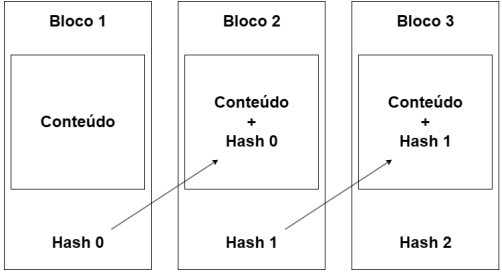
\includegraphics[width=0.7\textwidth]{diagrama_de_uma_blockchain.png}
    \legend{Fonte: \citeonline[p.~22]{souza2023}.}
\end{figure}

Não obstante essa contribuição seminal, \citeonline{nakamoto2008} não
abordou contratos inteligentes complexos nem aplicações voltadas à
autenticação ou assinatura de documentos, concentrando-se
exclusivamente no problema de moeda eletrônica e no modelo de
segurança associado. A literatura subsequente ampliou o escopo da
\emph{blockchain} para domínios como certificação acadêmica,
verificação de credenciais e autenticação documental, mas permanece a
lacuna de soluções orientadas à automação de fluxos de assinatura via
link em processos administrativos específicos, como a emissão e
assinatura do DFD. O presente trabalho, ao utilizar a
\emph{blockchain} como infraestrutura de registro imutável do
\emph{hash} de documentos assinados, contribui para preencher esse
espaço, explorando uma aplicação prática que extrapola o uso original
concebido por \citeonline{nakamoto2008}.

\section{Smart Contracts: Conceito, Origens e Funcionamento}

O conceito de \emph{smart contracts} foi formulado por
\citeonline{szabo1997}, que os definiu como protocolos computacionais
capazes de executar automaticamente os termos de um acordo, quando
determinadas condições pré-programadas são satisfeitas. A
contribuição de Szabo reside em transpor para o âmbito digital a
lógica de contratos autoexecutáveis, reduzindo a dependência de
intermediários e minimizando riscos de descumprimento por meio da
automatização das obrigações contratuais. Essa concepção abstrata
antecipou o uso de estruturas de dados e regras de negócio codificadas
para regular transações de maneira previsível e verificável.

Contudo, o trabalho de \citeonline{szabo1997} não apresentou uma infraestrutura
concreta de implementação, tampouco discutiu cenários específicos de
formalização documental ou fluxos de assinatura eletrônicos baseados em
links únicos, limitando-se a um modelo conceitual de contratos
autoexecutáveis. A viabilidade prática dos \emph{smart contracts} foi
consolidada apenas com o surgimento de plataformas como o Ethereum,
que disponibilizaram uma máquina virtual e uma linguagem de
programação apropriada para implementação desses protocolos. Ainda
assim, parte relevante da literatura concentra-se em aspectos
técnicos internos aos contratos, deixando em aberto a integração
entre esses mecanismos e interfaces de usuário simplificadas,
voltadas a fluxos de assinatura de documentos de negócios, como o
DFD. O sistema proposto, ao vincular \emph{smart contracts} a um
processo de assinatura via link, contribui para operacionalizar o
conceito de Szabo em um contexto aplicado e orientado ao usuário
final.

\section{Plataforma Ethereum e a Linguagem Solidity}
\label{sec:ethereum}

O \emph{white paper} ``A Next Generation Smart Contract \&
Decentralized Application Platform'', de Vitalik Buterin
\cite{buterin2014}, introduziu o Ethereum como uma plataforma de
\emph{blockchain} de propósito geral, dotada de uma linguagem
Turing-completa para a criação de contratos inteligentes e
aplicações descentralizadas (DApps). A principal contribuição do
Ethereum foi expandir o uso da \emph{blockchain} para além da
criptomoeda, permitindo que desenvolvedores definissem e executassem
lógicas de negócio arbitrárias na Ethereum Virtual Machine (EVM), por
meio de idiomas como a linguagem Solidity. Essa abordagem tornou
possível codificar regras de validação, armazenamento de estados e
emissão de eventos relacionados a transações complexas, incluindo o
registro de \emph{hashes} de documentos, dados de assinaturas e
metadados associados.

Apesar de viabilizar uma ampla gama de aplicações, o \emph{white
paper} de \citeonline{buterin2014} não apresenta uma aplicação específica voltada à
autenticação ou assinatura de documentos com interface \emph{web},
nem detalha padrões de desenho para sistemas de assinatura via link
que abstraiam a complexidade da \emph{blockchain} para usuários não
técnicos. A literatura técnica sobre Ethereum, em grande parte,
concentra-se em desafios de escalabilidade, segurança e custos de
transação (\emph{gas}), deixando em segundo plano a integração entre
contratos inteligentes e camadas de aplicação orientadas a processos
administrativos concretos, como a emissão e assinatura do DFD em
ambientes organizacionais. O trabalho em desenvolvimento utiliza a
infraestrutura do Ethereum e a linguagem Solidity para implementar um
contrato inteligente responsável por registrar, na rede, o
\emph{hash} do documento e o evento de assinatura associado ao link
enviado ao signatário, avançando em direção a uma solução prática que
Buterin apenas vislumbrou em termos genéricos.

Uma análise crítica da Ethereum mostra que sua adoção para fluxos
documentais não pode ser tratada apenas como escolha natural de
mercado. O modelo de execução baseado em gas introduz custo variável
por operação, o que afeta a previsibilidade orçamentária do sistema;
além disso, a escalabilidade da camada principal continua limitada
para aplicações que dependem de alto volume de interações ou
confirmação rápida em massa. Por essa razão, a literatura recente e a
prática do ecossistema passaram a tratar soluções de segunda camada,
ou \emph{Layer 2}, como alternativa relevante para reduzir custos e ampliar
\emph{throughput}, preservando parte das garantias de segurança da rede
principal.

Para o fluxo de assinatura via link aplicado ao DFD, isso significa
que a Ethereum deve ser compreendida como base tecnológica com
vantagens e \emph{trade-offs}. Sua segurança é elevada em razão da robustez
do ecossistema, da ampla auditoria pública e da maturidade das
ferramentas, mas a adoção direta da camada principal pode ser
excessiva para todas as etapas do processo. Assim, uma arquitetura
mais coerente tende a reservar a blockchain para o registro de
evidências essenciais, enquanto metadados operacionais e etapas de
interface permanecem fora da cadeia, admitindo inclusive futura
migração para redes L2 ou permissionadas conforme critérios de custo,
desempenho e governança.

\section{Assinaturas Digitais: Conceitos e Infraestrutura de Chave Pública}

Os modelos tradicionais de assinatura digital baseiam-se em
Infraestruturas de Chaves Públicas (PKI), nas quais autoridades
certificadoras centralizadas emitem certificados que vinculam a
identidade de um signatário a um par de chaves criptográficas
\cite{cooper2008}. Nesse contexto, obras de referência em criptografia
discutem o uso de funções \emph{hash}, criptossistemas de chave pública
e esquemas de assinatura digital (como RSA e ECDSA) para garantir
autenticidade, integridade e não repúdio em documentos eletrônicos
\cite{stallings2017}. Essas abordagens
estabelecem a base teórica para o uso de assinaturas digitais na
proteção de documentos e transações, e influenciam diretamente as
normas regulatórias, inclusive no Brasil, onde a ICP-Brasil e
legislações específicas classificam e disciplinam diferentes tipos de
assinaturas eletrônicas.

Entretanto, a literatura focada em PKI tradicional evidencia
limitações relevantes no que se refere à centralização, custos
recorrentes, pontos únicos de falha e dependência de autoridades
certificadoras, o que pode restringir a escalabilidade e a
acessibilidade de soluções baseadas exclusivamente nesse modelo. Além
disso, tais modelos não exploram de forma aprofundada a integração
entre assinaturas digitais e \emph{blockchain}, especialmente em
arquiteturas que pretendem combinar garantias de integridade e não
repúdio com registros distribuídos e verificáveis por qualquer parte.

O presente trabalho busca aproveitar os mecanismos criptográficos
consagrados (como o uso de \emph{hashes} e assinaturas assimétricas)
em conjunto com a \emph{blockchain} Ethereum, de modo a descentralizar
o registro das evidências de assinatura do DFD e reduzir a
dependência de autoridades centrais, ao mesmo tempo em que mantém a
compatibilidade com requisitos jurídicos e de comprovação documental.

\subsection{Conceitos de Infraestrutura de Chaves Públicas}

Uma Infraestrutura de Chaves Públicas (\emph{Public Key
Infrastructure} -- PKI) é um conjunto de políticas, papéis,
procedimentos e sistemas técnicos responsáveis por criar, gerenciar,
distribuir, armazenar e revogar certificados digitais, bem como
administrar chaves públicas. Seu elemento central é a Autoridade
Certificadora (AC), entidade confiável que atesta, por meio da
emissão de um certificado digital, o vínculo entre uma chave pública
e a identidade de seu titular. O certificado digital, normatizado
internacionalmente pelo padrão X.509, contém a chave pública do
titular, dados de identificação, o período de validade, o
identificador da AC emissora e a assinatura digital da própria AC
sobre esses dados, permitindo a formação de uma cadeia de confiança
(\emph{chain of trust}) que pode ser reconduzida até uma âncora de
confiança previamente aceita pelo verificador \cite{cooper2008}.
Outros elementos centrais de uma PKI incluem a Autoridade de Registro
(AR), responsável por validar a identidade do solicitante antes da
emissão do certificado, e as Listas de Certificados Revogados (CRL)
ou o protocolo OCSP, mecanismos que permitem verificar se um
certificado foi revogado antes do seu vencimento \cite{cooper2008}.

No Brasil, a Infraestrutura de Chaves Públicas Brasileira (ICP-Brasil)
foi instituída pela Medida Provisória n\textsuperscript{o} 2.200-2, de
24 de agosto de 2001, constituindo uma PKI hierárquica de âmbito
nacional, tendo o Instituto Nacional de Tecnologia da Informação
(ITI) como Autoridade Certificadora Raiz (AC-Raiz), com presunção de
veracidade atribuída aos documentos eletrônicos certificados nesse
âmbito \cite{brasil2001}. A Lei n\textsuperscript{o} 14.063, de 23 de
setembro de 2020, complementa essa infraestrutura ao disciplinar o
uso de assinaturas eletrônicas em interações com entes públicos,
classificando-as em assinatura eletrônica simples, avançada e
qualificada, esta última correspondendo às assinaturas baseadas em
certificados ICP-Brasil \cite{brasil2020}.

\subsection{Algoritmos Clássicos de Assinatura Digital}

Os esquemas de assinatura digital empregados em PKIs tradicionais
fundamentam-se em criptografia assimétrica, na qual a chave privada
do signatário é utilizada para gerar a assinatura sobre o hash da
mensagem, e a chave pública correspondente permite a qualquer parte
verificar essa assinatura. Entre os algoritmos consolidados,
destaca-se o RSA, proposto originalmente por
\citeonline{rivest1978}, cuja segurança baseia-se na dificuldade
computacional de fatorar números inteiros grandes resultantes do
produto de dois números primos; para oferecer níveis de segurança
adequados, o RSA exige chaves relativamente longas, de 2048 bits ou
mais \cite{nist2023}. O ECDSA (\emph{Elliptic Curve Digital Signature
Algorithm}), por sua vez, é uma variante de assinatura baseada em
criptografia de curvas elípticas, padronizada pelo NIST junto com o
RSA e o EdDSA como técnicas oficiais para geração e verificação de
assinaturas digitais \cite{nist2023}; para um nível de segurança
equivalente, requer chaves significativamente menores que o RSA, o
que o tornou o algoritmo padrão em diversas blockchains, incluindo a
Ethereum, que utiliza especificamente a curva secp256k1. Já o EdDSA
(\emph{Edwards-curve Digital Signature Algorithm}), em particular sua
instanciação Ed25519, foi proposto por \citeonline{bernstein2012}
como alternativa que corrige limitações de projeto do ECDSA, como
a dependência de um número aleatório (\emph{nonce}) gerado a cada
assinatura, cuja falha de geração pode comprometer a chave privada.
Além disso, o EdDSA é determinístico e apresenta alto desempenho, com os
autores relatando a geração de mais de cem mil assinaturas por
segundo em hardware comercial da época \cite{bernstein2012}; o
algoritmo foi posteriormente incorporado ao padrão oficial do NIST
\cite{nist2023}.

\subsection{Comparação entre Assinatura Digital Tradicional e Baseada em Blockchain}
\label{sec:comparacao-pki}

A literatura recente sobre PKIs baseadas em blockchain aponta que o
modelo centralizado de Autoridades Certificadoras carrega riscos
estruturais: uma AC comprometida pode emitir certificados fraudulentos
para servidores maliciosos, colocando em risco a privacidade e a
integridade dos dados dos usuários, e uma vez comprometida pode
derrubar toda a cadeia de confiança da PKI que dela depende
\cite{halder2024}. Nesse contexto, propostas de PKI
descentralizada substituem ou complementam a AC central por um
registro distribuído, aproveitando características intrínsecas da
blockchain, como imutabilidade, transparência e consenso descentralizado,
para viabilizar o registro, a distribuição e a revogação de
chaves sem depender de uma autoridade central \cite{halder2024}.
A implementação de uma PKI descentralizada na rede Ethereum,
apresentada por \citeonline{halder2024}, mostrou que é possível
emitir e revogar certificados sem depender de uma autoridade
certificadora e impedir a adulteração de certificados existentes,
ainda que com custo adicional de processamento em relação às PKIs
convencionais. O
Quadro~\ref{quadro:pki-blockchain} sintetiza as principais diferenças
entre a PKI tradicional e a abordagem baseada em blockchain quanto ao
modelo de confiança, ao vínculo entre identidade e chave, aos pontos
únicos de falha, à verificação de revogação, aos algoritmos empregados
e ao reconhecimento jurídico.

Essa comparação evidencia que a proposta de descentralizar o registro
das evidências de assinatura do DFD por meio da blockchain Ethereum
não substitui os fundamentos criptográficos da PKI, mas reconfigura o
modelo de confiança e de auditabilidade: em vez de depender
exclusivamente da disponibilidade e da integridade de uma AC central,
o sistema passa a apoiar-se em um registro distribuído, imutável e
verificável por qualquer parte interessada \cite{halder2024}, sem,
contudo, eliminar a necessidade de mecanismos
complementares de vinculação de identidade para manter aderência aos
requisitos legais previstos na Lei n\textsuperscript{o} 14.063/2020
\cite{brasil2020}.

\FloatBarrier
\begin{quadro}[htb]
    \caption{Comparação entre a PKI tradicional e a blockchain}
    \label{quadro:pki-blockchain}
    \centering
    \begin{tabular}{>{\raggedright\arraybackslash}p{3.3cm}>{\raggedright\arraybackslash}p{4.9cm}>{\raggedright\arraybackslash}p{4.9cm}}
        \toprule
        \textbf{Aspecto} & \textbf{PKI tradicional} & \textbf{Blockchain (ex.: Ethereum)} \\
        \midrule
        Modelo de confiança &
        Centralizado, hierárquico (AC-Raiz $\rightarrow$ ACs intermediárias) \cite{cooper2008} &
        Descentralizado, distribuído entre nós da rede \cite{halder2024} \\
        \addlinespace
        Vínculo identidade--chave &
        Certificado X.509 emitido e atestado por uma AC \cite{cooper2008} &
        Endereço derivado diretamente da chave pública, sem atestação de identidade por padrão \\
        \addlinespace
        Ponto único de falha &
        AC comprometida pode invalidar toda a cadeia de confiança abaixo dela \cite{halder2024} &
        Ausência de autoridade central; falha exige comprometer o consenso distribuído \\
        \addlinespace
        Verificação de revogação &
        Depende de CRL/OCSP \cite{cooper2008} &
        Registro imutável e publicamente auditável \cite{halder2024} \\
        \addlinespace
        Algoritmo típico &
        RSA, ECDSA \cite{nist2023} &
        ECDSA sobre secp256k1 (Ethereum) \\
        \addlinespace
        Reconhecimento jurídico &
        Consolidado no âmbito da ICP-Brasil \cite{brasil2001, brasil2020} &
        Em consolidação normativa \\
        \bottomrule
    \end{tabular}
    \legend{Fonte: elaborado pelo autor.}
\end{quadro}
\FloatBarrier

\section{Verificação e Autenticação de Documentos com Blockchain}

Diversos estudos recentes investigam o uso da \emph{blockchain} para
registro e verificação de documentos digitais, propondo soluções que
utilizam o armazenamento do \emph{hash} de arquivos na cadeia de
blocos como evidência de integridade e existência em determinado
momento. A prova de conceito de \citeonline{pedrosa2025} para um
sistema de registros acadêmicos em ensino superior, por exemplo,
demonstra a aplicação da \emph{blockchain} para armazenar e gerenciar
registros acadêmicos, como notas e históricos escolares, assegurando a
sua integridade e oferecendo aos estudantes acesso verificado às
próprias informações. A contribuição desse tipo de
trabalho consiste em mostrar a viabilidade prática de sistemas que
registram metadados de documentos e permitem sua verificação
posterior sem necessidade de confiar em uma única instituição
emissora, o que pode inspirar soluções semelhantes para documentos
contratuais e administrativos.

\citeonline{sotnykov2025}, por sua vez, apresenta um sistema de código
aberto para a verificação descentralizada de documentos por meio de
\emph{smart contracts}, no qual o \emph{hash} do documento é calculado
localmente pelo usuário e apenas essa prova criptográfica é registrada
na \emph{blockchain}, sem armazenar o conteúdo do documento, o que
reduz a dependência de entidades centrais e preserva a
confidencialidade. Tais propostas, ao
utilizarem \emph{hashes} criptográficos e contratos inteligentes,
demonstram que é possível garantir confiança documental em redes
distribuídas, ampliando o escopo de aplicação da \emph{blockchain}
para além de transações financeiras. No entanto, essas soluções não
contemplam, de forma abrangente, a integração com fluxos completos de
assinatura eletrônica via link, nem abordam os requisitos de usabilidade
e integração com sistemas organizacionais legados, como seria o caso
da automação do DFD em instituições públicas ou empresas de serviços.
O sistema proposto pretende avançar nesse sentido ao conceber um
fluxo no qual a geração do link, o ato de assinatura e o registro em
\emph{blockchain} constituem partes de um processo único e
automatizado, orientado à formalização documental.

A ampliação desse debate exige diversidade de autores e conceitos
correlatos, especialmente em torno de \emph{timestamping}, notarização
descentralizada e prova de existência. O \emph{timestamping} agrega
valor porque associa o hash do documento a uma marca temporal
verificável, útil para demonstrar que determinado conteúdo existia em
dado momento \cite{haber1991}; a notarização descentralizada desloca a
confiança de uma entidade única para mecanismos distribuídos de
registro \cite{uikey2024}; e a prova de existência, por sua vez, opera
como evidência técnica de anterioridade sem necessariamente expor o
conteúdo integral do documento em rede pública \cite{sotnykov2025}.

Esses três elementos contribuem diretamente para o fluxo do DFD. Em
vez de apenas guardar um hash, a solução passa a constituir um
encadeamento probatório composto pelo documento original, seu resumo
criptográfico, a marca temporal e o evento de assinatura via link.
Com isso, a verificação documental deixa de ser uma etapa isolada e
passa a integrar a lógica de auditoria do processo, o que reforça a
rastreabilidade e a utilidade prática do sistema em contextos
administrativos e contratuais.

\section{Notarização Digital Descentralizada e Compartilhamento de Arquivos}

A notarização digital descentralizada amplia a verificação de
documentos para o ciclo de autenticação, assinatura e compartilhamento.
\citeonline{irimia2025} propõe uma infraestrutura descentralizada para a
notarização, a assinatura e o compartilhamento de documentos oficiais
com \emph{blockchain}, baseada em microsserviços, armazenamento
descentralizado e técnicas criptográficas, e avalia o desempenho, a
segurança e a usabilidade do protótipo em comparação com soluções
existentes, apontando o potencial da notarização digital para reduzir a
falsificação, a perda e o acesso não autorizado a documentos.
Diferentemente dessa infraestrutura, de escopo amplo, o presente
trabalho concentra-se no fluxo de assinatura via link, com o registro
da prova de existência do documento e das evidências da assinatura.

O Quadro~\ref{quadro:correlatos} compara os sistemas discutidos neste
capítulo com o sistema proposto quanto à finalidade, à rede utilizada
e aos dados nela registrados, à assinatura do documento por terceiros
e à exigência de carteira digital por parte do usuário. Foi incluído
também o trabalho de \citeonline{souza2023}, que registra na rede Celo
o \emph{hash} de documentos em PDF para a posterior verificação da sua
autenticidade; a revisão de \citeonline{uikey2024} não foi incluída,
por não propor um sistema. A comparação evidencia a lacuna explorada
neste trabalho: entre os sistemas analisados, apenas o de
\citeonline{irimia2025} contempla a assinatura do documento por
terceiros, e o faz com acesso principal pela carteira MetaMask, em uma
rede permissionada, enquanto o sistema proposto combina a assinatura
pelo signatário, por meio de link único e sem carteira digital, com o
registro em rede pública.

\begin{quadro}[htbp]
    \caption{Comparação entre trabalhos correlatos e o sistema proposto}
    \label{quadro:correlatos}
    \centering
    \small
    \begin{tabular}{L{2.4cm}L{3.0cm}L{3.6cm}L{2.2cm}L{2.6cm}}
        \toprule
        \textbf{Trabalho} & \textbf{Finalidade} & \textbf{Rede e dados registrados} & \textbf{Assinatura por terceiros} & \textbf{Carteira do usuário} \\
        \midrule
        \citeonline{souza2023} & Registro e verificação da autenticidade de documentos em PDF & Rede de testes da Celo; \emph{hash} SHA-256 do arquivo e metadados & Não & Não exigida; acesso por e-mail e senha \\
        \addlinespace
        \citeonline{pedrosa2025} & Registro de dados acadêmicos, como notas e históricos & Ethereum; dados acadêmicos, dados pessoais cifrados e \emph{hash} desses dados & Não & Exigida (MetaMask) \\
        \addlinespace
        \citeonline{sotnykov2025} & Prova de existência de documentos & Redes de testes Sepolia (Ethereum) e Amoy (Polygon); \emph{hash} do documento e metadados & Não & Exigida (MetaMask ou compatível) \\
        \addlinespace
        \citeonline{irimia2025} & Notarização, assinatura e compartilhamento de documentos oficiais & GoQuorum, rede permissionada baseada na Ethereum, com arquivos no IPFS; \emph{hash} dos documentos e fatos notarizados & Sim, por notário ou signatário autorizado & MetaMask, com alternativa por e-mail e senha \\
        \addlinespace
        Sistema proposto & Assinatura eletrônica de documentos via link & Rede de testes Sepolia (Ethereum); \emph{hash} do documento e \emph{hash} das evidências & Sim, pelo signatário, por link único & Não exigida \\
        \bottomrule
    \end{tabular}
    \legend{Fonte: elaborado pelo autor.}
\end{quadro}
\FloatBarrier

No plano jurídico nacional, convém reforçar que a discussão não se
esgota na validade abstrata do contrato inteligente, mas alcança a
validade probatória das evidências geradas e a responsabilidade pelos
atos praticados no sistema. A liberdade probatória prevista no art.
369 do Código de Processo Civil \cite{brasil2015} amplia a admissibilidade de registros
digitais, inclusive em blockchain, mas não elimina a necessidade de
demonstrar cadeia de custódia informacional, autoria do ato,
integridade do documento e confiabilidade do procedimento técnico
empregado.

Também é necessário diferenciar, com maior precisão, assinatura
eletrônica simples, avançada e qualificada, pois cada categoria
produz efeitos distintos quanto à robustez da identificação e ao peso
probatório do documento \cite{brasil2020}. Nessa perspectiva, a
validade de documentos eletrônicos depende da combinação entre técnica,
contexto de uso, governança do sistema e suficiência das evidências
produzidas. Para o DFD, isso
significa que a assinatura via link pode ser juridicamente útil e
probatoriamente relevante, mas sua força dependerá do desenho de
segurança, do nível de autenticação adotado e da possibilidade de
atribuição de responsabilidade em caso de contestação.

\section{Desafios Técnicos em Smart Contracts: Segurança, Privacidade e Performance}
\label{sec:desafios}

A literatura técnica sobre \emph{smart contracts} identifica
múltiplos desafios relacionados a codificação, segurança, privacidade
e desempenho, destacando que vulnerabilidades no código podem
resultar em perdas financeiras, violações de integridade e
comportamentos inesperados em aplicações descentralizadas
\cite{alharby2017}. O mapeamento sistemático da pesquisa em contratos
inteligentes realizado por \citeonline{alharby2017} organizou o estado da arte e apontou lacunas em temas como
verificação formal, testes automatizados e mecanismos de proteção
contra ataques, além de ressaltar questões de escalabilidade e custos
de transação em redes públicas. A principal contribuição desse tipo
de estudo é fornecer um panorama abrangente dos riscos e boas
práticas, orientando a comunidade acadêmica e profissional na busca
por soluções mais seguras e eficientes.

Complementarmente, o mesmo mapeamento reúne as soluções propostas
para esses problemas: métodos de verificação formal, capazes de
revelar comportamentos não previstos antes da publicação do contrato;
materiais de orientação para a escrita de contratos corretos; e
ferramentas automatizadas, como a Oyente, que identifica contratos
vulneráveis à dependência da ordem das transações, à dependência do
horário do bloco, ao tratamento inadequado de exceções e à
reentrância, e a Gasper, que identifica contratos com consumo de
\emph{gas} não otimizado \cite{alharby2017}. Os autores observam, contudo, que
parte dessas soluções não passou de propostas sem avaliação concreta e
que alguns problemas permanecem sem solução. No campo específico das
assinaturas digitais, a integração da \emph{blockchain} com
infraestruturas de chaves públicas permite emitir e revogar
certificados sem depender de uma autoridade certificadora, ainda que
com custo adicional de processamento \cite{halder2024}. O presente
trabalho incorpora essas preocupações ao adotar práticas de
desenvolvimento prudentes em Solidity, cuja aplicação ao contrato
desenvolvido é examinada no Capítulo~\ref{sec:res-contrato}, ao
projetar um \emph{backend} que abstrai a complexidade das
transações e ao conceber uma interface que minimiza a exposição do
usuário a detalhes técnicos, buscando equilibrar segurança
criptográfica, desempenho e experiência de uso no fluxo de assinatura
do DFD.

\section{Desenvolvimento Web para Interfaces de Assinatura Eletrônica}
\label{sec:web}

Os sistemas de assinatura eletrônica baseados em \emph{blockchain} e
\emph{smart contracts} dependem, para sua adoção prática, de
interfaces \emph{web} que ofereçam uma experiência de uso intuitiva,
carteiras digitais e taxas de transação. Na literatura revisada,
observa-se que diversas provas de conceito e protótipos utilizam
\emph{frontends} desenvolvidos com tecnologias \emph{web} modernas,
integrados a \emph{backends} em plataformas como Node.js, a fim de
interagir com contratos inteligentes e redes \emph{blockchain}. Esses
trabalhos demonstram a viabilidade de expor funcionalidades de
registro e verificação de documentos por meio de interfaces gráficas
acessíveis, aproximando o usuário da tecnologia subjacente.

Entretanto, muitas dessas soluções mantêm uma forte dependência da
interação direta com carteiras digitais (como MetaMask) e exigem que
o usuário compreenda conceitos como \emph{wallets}, \emph{gas fees} e
seleção de redes, o que constitui uma barreira importante para adoção
em massa. Além disso, a literatura raramente aborda, de forma
sistemática, o desenho de fluxos de uso específicos para automação de
processos administrativos, como a geração e o acompanhamento de
assinaturas em documentos preparatórios do tipo DFD. O sistema
proposto neste trabalho busca mitigar tais limitações por meio de um
\emph{backend} em Node.js que gerencia as interações com a
\emph{blockchain} e de uma interface \emph{web} que permite ao
remetente gerar e enviar links de assinatura, bem como monitorar o
status do DFD, sem expor o signatário à complexidade técnica da
infraestrutura subjacente.

Sob a perspectiva de desenvolvimento web, a literatura técnica de UX
e segurança mostra que a adoção de sistemas sensíveis depende da
redução de fricção cognitiva e da comunicação clara de risco. Em
interfaces da assinatura, elementos como confirmação explícita do
documento, indicação do status do processo, mensagens compreensíveis
de erro, prevenção de ações acidentais e design responsivo deixam de
ser apenas escolhas estéticas e passam a compor a segurança
operacional do sistema.

No fluxo de assinatura via link, a interface precisa equilibrar
simplicidade e garantias mínimas de confiança. Isso implica
apresentar o documento de forma verificável, evidenciar o vínculo
entre link e ato de assinatura, proteger dados de sessão, adotar
transporte seguro, controles contra reutilização indevida e
mecanismos de confirmação compatíveis com o perfil do usuário não
técnico. Em outras palavras, a camada web não é acessória ao problema
do DFD, mas parte estrutural da credibilidade prática da solução.

\section{Geração e Gerenciamento de Links Únicos para Coleta de Assinatura}
\label{sec:links}

A geração e o gerenciamento de links únicos constituem elemento
central da proposta deste trabalho, pois materializam a automação da
fase preparatória da formalização documental, em que o Documento de
Formalização da Demanda (DFD) é encaminhado para coleta de assinaturas
de maneira remota. Embora parte da literatura sobre notarização digital
e autenticação documental com \emph{blockchain} contemple o envio de
documentos e a verificação por usuários externos, poucos estudos
descrevem detalhadamente mecanismos de criação de links exclusivos
que vinculem, de forma inequívoca, um signatário, um documento e um
registro em \emph{blockchain}. Em geral, os trabalhos focam na prova
de existência e integridade do documento, sem especificar fluxos de
\emph{tokens} de acesso ou URL parametrizadas para coleta de
concordância de forma simplificada.

O DFD é um instrumento próprio das contratações públicas. Previsto na
Lei n\textsuperscript{o} 14.133, de 2021, como base para a elaboração
do plano de contratações anual dos órgãos e entidades
\cite{brasil2021}, foi regulamentado, no âmbito da administração
pública federal, pelo Decreto n\textsuperscript{o} 10.947, de 2022,
que o define como o documento que fundamenta o plano de contratações
anual e no qual a área requisitante evidencia e detalha a necessidade
de contratação \cite{brasil2022}. Trata-se, portanto, do ato que dá
início à fase preparatória do processo de contratação. Segundo o
mesmo decreto, o DFD deve conter a justificativa da necessidade, a
descrição sucinta do objeto, a quantidade a ser contratada, a
estimativa preliminar do valor, a data pretendida para a conclusão da
contratação e a identificação da área requisitante e do responsável
pela demanda \cite{brasil2022}. Por exigir a identificação desse
responsável, cuja assinatura formaliza o documento, o DFD constitui um
caso representativo de documento cuja tramitação depende da coleta de
assinaturas, o que motiva sua adoção como foco inicial do sistema
proposto. O fluxo de assinatura via link, contudo, não se restringe a
esse documento, aplicando-se igualmente a contratos, termos e demais
documentos que demandem a formalização remota da concordância de uma
das partes.

A lacuna descrita no início desta seção torna-se particularmente
relevante quando se considera o
contexto de uso em setores como seguros, serviços e Administração
Pública, nos quais o DFD e documentos análogos precisam ser assinados
por partes que nem sempre dispõem de certificação digital ou
familiaridade com carteiras de criptomoedas. A literatura aponta a
necessidade de soluções que conciliem segurança criptográfica,
usabilidade e integração com processos regulados, mas não apresenta
um modelo consolidado de gestão de links de assinatura baseado em
\emph{smart contracts}. O sistema proposto, ao combinar geração de
links únicos na camada de \emph{backend}, registro imutável do
\emph{hash} do documento e do \emph{hash} das evidências da assinatura
na \emph{blockchain} Ethereum e interface \emph{web} para monitoramento
do fluxo, posiciona-se como contribuição inovadora nesse espaço,
buscando preencher a lacuna entre modelos teóricos de autenticação
documental e a prática da automação da fase preparatória de
formalização de demandas.

O aprofundamento dessa seção exige destacar que o link único
concentra parcela sensível do risco de segurança do sistema. Entre as
ameaças mais relevantes estão \emph{phishing}, interceptação do link
em canais inseguros, reutilização indevida, expiração inadequada e
uso de \emph{tokens} previsíveis ou mal protegidos. Se o elo de
acesso for comprometido, a robustez do registro em \emph{blockchain}
não impede, por si só, o problema de atribuição indevida do ato ao
suposto signatário.

Por isso, a lacuna identificada na literatura é mais específica do
que a mera ausência de links de assinatura. O ponto ainda pouco
desenvolvido está na combinação entre geração segura de tokens,
controle temporal de validade, política de uso único, associação
contextual entre destinatário e documento, registro auditável do
evento de acesso e integração dessas evidências com o contrato
inteligente. Para o DFD, essa lacuna é decisiva, porque a utilidade de
uma assinatura via link depende de mecanismos que conciliem
conveniência de acesso com segurança suficiente para sustentar
integridade, rastreabilidade e valor probatório do fluxo.

% =================================================================
\chapter{Metodologia}
% =================================================================

Este capítulo descreve os procedimentos metodológicos adotados para
responder à pergunta de pesquisa formulada no Capítulo 1 e alcançar os
objetivos propostos. Inicialmente, o Capítulo~\ref{sec:tipo-pesquisa}
caracteriza a pesquisa quanto à natureza, à abordagem e aos
procedimentos técnicos. Em seguida, o Capítulo~\ref{sec:proc-metodologicos}
detalha os métodos de coleta e de análise das informações que
fundamentaram o trabalho. O Capítulo~\ref{sec:metodologia-desenvolvimento}
apresenta a metodologia de desenvolvimento do sistema, compreendendo
o modelo de desenvolvimento de \emph{software}, as tecnologias
utilizadas e a arquitetura adotada. Por fim, o
Capítulo~\ref{sec:testes} estabelece os procedimentos de teste e
validação do protótipo, definindo os tipos de testes, os cenários, as
métricas coletadas e os critérios de aceitação.

\section{Tipo de Pesquisa}
\label{sec:tipo-pesquisa}

A pesquisa desenvolvida neste trabalho caracteriza-se, de forma
geral, como uma pesquisa aplicada e de orientação projetual, na
medida em que parte da identificação de uma lacuna prática
relacionada à assinatura remota de documentos e busca produzir, como
resultado, um artefato computacional funcional capaz de registrar
evidências de assinatura em blockchain, e não apenas ampliar o
conhecimento teórico sobre o tema \cite{nakamoto2008, buterin2014,
szabo1997}.

\subsection{Natureza da pesquisa}

Quanto à natureza, a pesquisa é aplicada, pois está voltada à geração
de conhecimento dirigido à solução de um problema concreto, a
dificuldade recorrente na coleta remota de assinaturas em documentos,
como o Documento de Formalização da Demanda (DFD), por meio da
concepção, especificação e implementação de um sistema de assinatura
eletrônica via link integrado a smart contracts na blockchain Ethereum.
Essa escolha se justifica porque o trabalho não se limita a discutir
teoricamente blockchain, smart contracts e assinaturas digitais, mas
propõe-se a desenvolver um protótipo funcional que materialize essas
tecnologias em uma solução de uso prático, atendendo ao objetivo
geral e aos objetivos específicos estabelecidos no Capítulo 1.

\subsection{Abordagem metodológica}

Quanto à abordagem, a pesquisa é predominantemente qualitativa, uma
vez que a maior parte de suas etapas, como a revisão do referencial
teórico, a análise dos trabalhos correlatos, a verificação funcional
do smart contract, a avaliação da usabilidade da interface e a
análise jurídica da solução frente ao ordenamento brasileiro,
baseia-se na interpretação e na análise qualitativa de informações,
conforme sintetizado no delineamento metodológico do
Quadro~\ref{quadro:delineamento}. Complementarmente, a pesquisa
incorpora elementos quantitativos exploratórios na etapa de avaliação
do protótipo, referentes à coleta de métricas de desempenho das
transações registradas na blockchain, o que caracteriza uma
abordagem mista, com predominância qualitativa.

\begin{quadro}[htb]
    \caption{Delineamento metodológico da pesquisa}
    \label{quadro:delineamento}
    \centering
    \begin{tabular}{ll}
        \toprule
        \textbf{Critério} & \textbf{Classificação} \\
        \midrule
        Natureza & Pesquisa aplicada \\
        Abordagem & Qualitativa, com elementos quantitativos exploratórios \\
        Objetivos & Descritiva / projetual \\
        Procedimentos técnicos & Desenvolvimento experimental \\
        \bottomrule
    \end{tabular}
    \legend{Fonte: elaborado pelo autor.}
\end{quadro}

\subsection{Procedimentos técnicos}
\label{sec:procedimentos-tecnicos}

Os procedimentos técnicos combinam pesquisa bibliográfica e desenvolvimento experimental, conforme o Quadro~\ref{quadro:delineamento}. A pesquisa bibliográfica, apresentada no Capítulo 2, analisou a literatura sobre blockchain, smart contracts e PKI, identificando a lacuna que justifica o projeto: a ausência de soluções que integrem smart contracts na Ethereum a um mecanismo simples de assinatura via link \cite{buterin2014,alharby2017}.

O desenvolvimento experimental corresponde à construção do artefato em três frentes: (i) smart contracts em Solidity para registrar o hash do documento e o hash das evidências da assinatura na Ethereum; (ii) backend em Node.js, intermediando aplicação web e blockchain; e (iii) interface web para geração, envio e acompanhamento dos links.

Esse caráter experimental exige testar o protótipo quanto a segurança, integridade, desempenho e usabilidade \cite{stallings2017}, critérios detalhados no Capítulo~\ref{sec:testes}. A escolha decorre da própria pergunta de pesquisa, que demanda validação empírica de um sistema funcional, não apenas análise teórica.

\section{Procedimentos Metodológicos}
\label{sec:proc-metodologicos}

Uma vez definidos, no Capítulo~\ref{sec:tipo-pesquisa}, a natureza da pesquisa e os procedimentos técnicos adotados, cabe detalhar como o estudo foi efetivamente conduzido, desde a coleta das informações que fundamentaram o projeto até a forma como essas informações foram analisadas e traduzidas em decisões de arquitetura e implementação do sistema proposto. Essa etapa articula a revisão da literatura apresentada no Capítulo 2 com as escolhas técnicas detalhadas no Capítulo 4, funcionando como elo metodológico entre a fundamentação teórica e o desenvolvimento do artefato.

\subsection{Métodos de coleta de informações}

A coleta de informações que sustenta este trabalho baseou-se, primordialmente, em pesquisa bibliográfica realizada em fontes acadêmicas primárias e secundárias relacionadas à tecnologia blockchain, aos smart contracts e às infraestruturas de assinatura digital. Foram consultados os trabalhos seminais que estabeleceram os fundamentos conceituais da área, como a proposta original de \citeonline{nakamoto2008} para o registro distribuído de transações, a formulação de \citeonline{szabo1997} para contratos autoexecutáveis e o white paper de \citeonline{buterin2014} sobre a plataforma Ethereum. Também foram consultados a literatura técnica de referência em criptografia e segurança da informação \cite{stallings2017} e estudos específicos sobre PKI, tanto em seu modelo tradicional centralizado \cite{cooper2008} quanto em propostas de descentralização baseadas em blockchain.

Complementarmente, a coleta envolveu a análise de trabalhos correlatos que tratam da verificação e autenticação de documentos em blockchain, da notarização digital descentralizada e dos desafios técnicos relacionados à segurança, à privacidade e ao desempenho de smart contracts \cite{alharby2017,zheng2018}, permitindo mapear soluções já existentes e identificar, por contraste, a lacuna específica que este trabalho se propõe a preencher. Também foram consultados dispositivos normativos brasileiros pertinentes ao tema, notadamente a Medida Provisória n\textsuperscript{o} 2.200-2/2001 \cite{brasil2001} e a Lei n\textsuperscript{o} 14.063/2020 \cite{brasil2020}, de modo a situar a proposta técnica dentro do arcabouço jurídico nacional relativo às assinaturas eletrônicas.

O trabalho não envolve coleta de dados primários por meio de entrevistas, questionários ou observação direta de usuários. Os dados empíricos provêm do próprio funcionamento do protótipo, como as métricas de desempenho das transações registradas na blockchain e os resultados dos testes previstos no Capítulo~\ref{sec:testes}.

\subsection{Métodos de análise das informações}

As informações reunidas na etapa de coleta foram submetidas a análise qualitativa de natureza interpretativa, com o objetivo de identificar convergências, divergências e lacunas entre os trabalhos consultados. Esse processo envolveu, em um primeiro momento, a categorização da literatura por eixo temático, contemplando fundamentos de blockchain, funcionamento de smart contracts, infraestrutura de chave pública, verificação documental e aspectos jurídicos, o que permitiu organizar o referencial teórico de forma estruturada, conforme refletido no Capítulo 2.

Em um segundo momento, procedeu-se a uma análise crítica e comparativa entre os modelos tradicionais de assinatura digital baseados em PKI e as propostas emergentes de descentralização via blockchain, contrapondo vantagens e limitações de cada abordagem quanto a centralização, custos, pontos únicos de falha e verificação de revogação. Essa comparação, sistematizada de forma sintética no Quadro~\ref{quadro:pki-blockchain}, apresentado no Capítulo~\ref{sec:comparacao-pki}, forneceu subsídio direto para a justificativa técnica da escolha pela blockchain Ethereum como infraestrutura de registro do sistema proposto.

\section{Metodologia de Desenvolvimento do Sistema}
\label{sec:metodologia-desenvolvimento}

Definidos, no Capítulo~\ref{sec:proc-metodologicos}, os procedimentos metodológicos gerais da pesquisa, esta seção detalha o processo técnico específico adotado para a construção do sistema de assinatura eletrônica via link com registro imutável em blockchain, abrangendo o modelo de desenvolvimento de software, as tecnologias empregadas e a arquitetura geral da solução. Enquanto o Capítulo~\ref{sec:tipo-pesquisa} situa o trabalho no plano metodológico da pesquisa científica, esta seção descreve o planejamento do desenvolvimento propriamente dito, distinguindo-se do Capítulo 4, que apresentará a execução efetiva do que foi construído.

\subsection{Modelo de desenvolvimento de software}

O desenvolvimento do sistema adota o método Kanban, combinado a uma estratégia de entregas incrementais. O Kanban é um método de gestão do trabalho apoiado na visualização do fluxo de atividades, na limitação da quantidade de trabalho em andamento e no acompanhamento contínuo desse fluxo, promovendo melhorias graduais no processo sem impor papéis ou cerimônias fixas \cite{anderson2010}. A escolha decorre da natureza do projeto. Por se tratar de um trabalho desenvolvido individualmente, métodos que pressupõem uma equipe com papéis definidos, como o Scrum, exigiriam adaptações significativas, ao passo que o Kanban pode ser aplicado diretamente por um único desenvolvedor. Além disso, a implementação de contratos inteligentes exige ciclos curtos de codificação, teste e validação, em razão da imutabilidade do código publicado na blockchain \cite{buterin2014}, o que favorece um processo iterativo em vez de modelos sequenciais rígidos, do tipo cascata.

Na aplicação ao projeto, as atividades são organizadas em um quadro com as colunas A fazer, Em andamento e Concluído, e o trabalho em andamento é limitado a poucas tarefas simultâneas, de modo que cada funcionalidade seja concluída antes do início da seguinte. O sistema é construído em quatro incrementos funcionais, cada um resultando em uma parte utilizável e testada da solução: (i) estrutura do projeto e banco de dados; (ii) envio do documento e geração do link único de assinatura; (iii) interface de assinatura e coleta de evidências; e (iv) integração com a blockchain Ethereum por meio do contrato inteligente. Ao final de cada incremento, as funcionalidades entregues são verificadas em relação aos requisitos especificados no Capítulo~\ref{sec:requisitos}, e eventuais ajustes são incorporados aos incrementos seguintes.

\subsection{Tecnologias utilizadas}

A definição das tecnologias empregadas no desenvolvimento do sistema decorre diretamente dos objetivos específicos estabelecidos no Capítulo 1 e do referencial teórico apresentado no Capítulo 2, contemplando as três camadas do diagrama de blocos da Figura~\ref{fig:arquitetura}: a \elem{Camada de registro distribuído}, a \elem{Camada de aplicação} e a \elem{Camada de apresentação}.

Na \elem{Camada de registro distribuído}, adotou-se a blockchain Ethereum como infraestrutura de execução dos contratos inteligentes, em razão de sua natureza de plataforma de propósito geral, dotada de linguagem Turing-completa e de uma máquina virtual, a Ethereum Virtual Machine (EVM), capaz de executar lógica de negócio arbitrária de forma descentralizada \cite{buterin2014}. Os contratos inteligentes responsáveis pelo registro do hash do documento e do hash das evidências da assinatura foram especificados na linguagem Solidity, escolhida por ser o padrão consolidado para desenvolvimento de contratos na rede Ethereum, com ampla documentação, maturidade de ferramentas e suporte a padrões de segurança amplamente auditados pela comunidade \cite{alharby2017}.

Na \elem{Camada de aplicação}, optou-se pelo desenvolvimento de um \emph{backend} em Node.js, responsável por gerenciar a geração e o controle de validade dos links únicos de assinatura, processar as requisições oriundas da interface web e intermediar a comunicação com a rede Ethereum, de modo a abstrair do usuário final, sobretudo do signatário, a complexidade técnica inerente às transações on-chain, tais como o gerenciamento de carteiras digitais e o pagamento de taxas de transação (\emph{gas fees}), conforme discutido no Capítulo~\ref{sec:web}.

Na \elem{Camada de apresentação}, foi concebida uma aplicação web destinada a dois perfis de usuário distintos: o remetente, que gera e acompanha os links de assinatura, e o signatário, que acessa o link para visualizar o documento e confirmar ou recusar a assinatura. A interface prioriza simplicidade de uso e comunicação clara do status do processo, em conformidade com o requisito de usabilidade RNF2, definido no Capítulo~\ref{sec:requisitos}.

Para a implementação, foram adotadas as seguintes ferramentas, todas de uso gratuito: o ambiente de execução Node.js, com o \emph{framework} Express, na construção do \emph{backend}; o sistema gerenciador de banco de dados relacional MySQL, acessado pela biblioteca mysql2, no armazenamento dos dados operacionais mantidos fora da cadeia, como documentos, links, evidências e situação de cada solicitação; a biblioteca ethers.js, na comunicação do \emph{backend} com a rede Ethereum; e as bibliotecas pdf-lib e PDF.js, empregadas, respectivamente, na geração da cópia do documento com a caixa de assinatura e na exibição do documento no navegador para o posicionamento dessa caixa. O contrato inteligente foi desenvolvido, compilado e testado no ambiente Remix IDE, primeiro na máquina virtual simulada oferecida pelo próprio ambiente, a Remix VM, e depois implantado, por meio da carteira MetaMask, na rede de testes Sepolia, uma rede pública da Ethereum na qual as transações são pagas com moeda de teste, sem valor financeiro. As versões efetivamente empregadas e a finalidade de cada ferramenta são detalhadas no Capítulo~\ref{sec:impl-tecnologias}.

\subsection{Arquitetura do sistema}
\label{sec:arquitetura}

A arquitetura do sistema proposto organiza-se segundo um modelo cliente-servidor estendido pela \elem{Camada de registro distribuído}, na qual a blockchain Ethereum atua como componente de confiança para o armazenamento imutável das evidências de assinatura, enquanto os demais componentes do sistema operam em infraestrutura convencional, centralizada, conforme ilustrado na Figura~\ref{fig:arquitetura}.

\begin{figure}[htb]
    \centering
    \caption{Diagrama de blocos da arquitetura do sistema}
    \label{fig:arquitetura}
    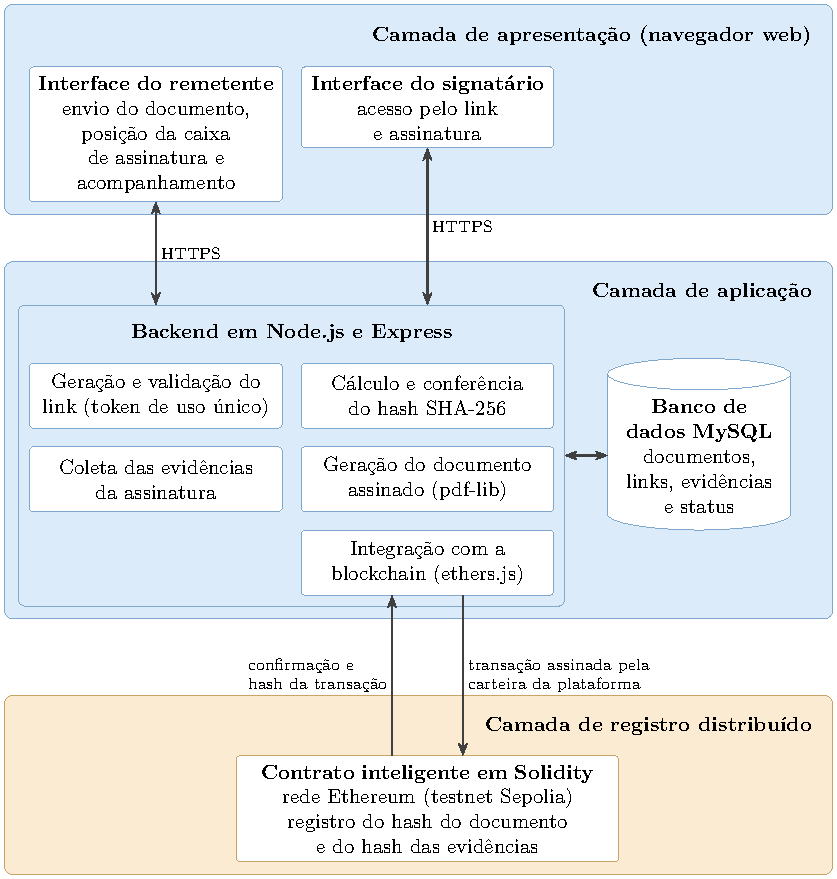
\includegraphics{diagrama_de_arquitetura.pdf}
    \legend{Fonte: elaborado pelo autor.}
\end{figure}

Essa arquitetura estrutura-se em três camadas principais: (i) a \elem{Camada de apresentação}, correspondente à interface web, composta pela \elem{Interface do remetente} e pela \elem{Interface do signatário}; (ii) a \elem{Camada de aplicação}, correspondente ao \elem{Backend em Node.js e Express}, responsável pela lógica de negócio e organizado nos módulos \elem{Geração e validação do link (token de uso único)}, \elem{Cálculo e conferência do hash SHA-256}, \elem{Coleta das evidências da assinatura}, \elem{Geração do documento assinado (pdf-lib)} e \elem{Integração com a blockchain (ethers.js)}, apoiada pelo \elem{Banco de dados MySQL} que armazena os documentos, os links, as evidências e o status de cada solicitação; e (iii) a \elem{Camada de registro distribuído}, correspondente ao \elem{Contrato inteligente em Solidity} implantado na rede Ethereum, responsável por persistir de forma imutável o hash do documento e o hash das evidências da assinatura, bem como por permitir sua consulta e verificação posterior, em atendimento aos requisitos RF4 e RF5 definidos no Capítulo~\ref{sec:requisitos}.

A separação entre metadados operacionais, armazenados fora da cadeia, e evidências criptográficas essenciais, registradas on-chain, reflete a análise crítica já desenvolvida no Capítulo~\ref{sec:ethereum} quanto aos \emph{trade-offs} de custo e desempenho da camada principal da Ethereum, reservando o uso da blockchain exclusivamente às informações cuja imutabilidade e auditabilidade pública são estritamente necessárias, ao passo que dados de sessão, controle de acesso ao link e demais informações operacionais permanecem sob gestão do backend. Essa decisão arquitetural preserva a possibilidade de, futuramente, migrar o registro para soluções de segunda camada (\emph{Layer 2}) ou redes permissionadas, conforme apontado no Capítulo~\ref{sec:ethereum}.

\FloatBarrier
\section{Procedimentos de Teste e Validação}
\label{sec:testes}

Definida, no Capítulo~\ref{sec:metodologia-desenvolvimento}, a metodologia de desenvolvimento do sistema, esta seção estabelece os procedimentos previstos para testar e validar o artefato resultante, de modo a verificar em que medida o protótipo atende aos requisitos funcionais e não funcionais especificados no Capítulo~\ref{sec:requisitos}, bem como à pergunta de pesquisa formulada no Capítulo 1. Em conformidade com o caráter de desenvolvimento experimental atribuído aos procedimentos técnicos deste trabalho no Capítulo~\ref{sec:procedimentos-tecnicos}, a validação do sistema constitui etapa indispensável, uma vez que a viabilidade técnica da proposta não pode ser demonstrada apenas por meio de sua especificação teórica, mas depende da avaliação empírica do funcionamento do protótipo implementado.

\subsection{Tipos de testes aplicados}

Estão previstos quatro tipos principais de testes, cada um voltado a uma dimensão específica de qualidade do sistema:
\begin{itemize}
\item Testes funcionais, destinados a verificar se as funcionalidades implementadas correspondem aos requisitos funcionais definidos no Capítulo~\ref{sec:requisitos} (RF1 a RF7), tais como a geração do link único de assinatura, a verificação da identidade do signatário por CPF e data de nascimento, a apresentação do documento ao signatário, a geração da cópia do documento com a caixa de assinatura preenchida, o registro do hash do documento e do hash das evidências no smart contract e a consulta posterior desse registro na blockchain.

\item Testes de integração, voltados a verificar a comunicação correta entre as três camadas da arquitetura do sistema descrita no Capítulo~\ref{sec:arquitetura}, isto é, a \elem{Camada de apresentação}, a \elem{Camada de aplicação} e a \elem{Camada de registro distribuído}, assegurando que requisições originadas na \elem{Camada de apresentação} sejam corretamente processadas pela \elem{Camada de aplicação} e refletidas, de forma consistente, no registro on-chain.

\item Testes de desempenho, direcionados à mensuração do tempo de resposta das operações do sistema, com especial atenção ao tempo de confirmação das transações registradas na blockchain Ethereum, de modo a avaliar sua compatibilidade com o uso em contexto comercial e administrativo cotidiano, conforme estabelecido no requisito não funcional RNF3.

\item Avaliação de usabilidade por inspeção da interface, realizada pelo autor, com o objetivo de verificar se o fluxo do signatário efetivamente abstrai a complexidade da blockchain, isto é, se pode ser concluído sem exigir carteira digital, pagamento de taxas de transação, instalação de software ou conhecimento técnico sobre blockchain, em atendimento ao requisito não funcional RNF2 e à discussão sobre redução de fricção cognitiva apresentada no Capítulo~\ref{sec:web}.
\end{itemize}
\subsection{Cenários de teste}
\label{sec:cenarios-teste}

Os cenários de teste devem contemplar tanto o fluxo principal de uso do sistema, descrito no diagrama de atividades da Figura~\ref{fig:atividades}, quanto seus fluxos alternativos e de exceção, de modo a avaliar o comportamento do sistema em condições adversas. Entre os cenários previstos, destacam-se:
\begin{itemize}

\item Geração de um link de assinatura válido, acesso pelo signatário e confirmação da assinatura, com verificação subsequente do registro correto do hash do documento e do hash das evidências na blockchain;

\item Tentativa de acesso a um link expirado ou já utilizado, verificando se o sistema impede corretamente a reutilização indevida, em conformidade com o requisito RNF5;

\item Informação de CPF ou data de nascimento incorretos pelo signatário, verificando se o documento permanece fechado enquanto os dados não coincidirem com os cadastrados pelo remetente, se a abertura é liberada quando os dados corretos são informados dentro do limite de três tentativas e se, esgotadas as três tentativas, o sistema registra a falha de identificação, altera o status do link para bloqueado e notifica o solicitante, em conformidade com o requisito RF6;

\item Posicionamento da caixa de assinatura no envio do documento e posterior assinatura, verificando se a cópia gerada apresenta a caixa na página e no local definidos pelo remetente, preenchida com o nome do signatário, a data e a hora da assinatura e o código de verificação, se o hash dessa cópia integra as evidências da assinatura e se o documento original permanece inalterado, em conformidade com o requisito RF7;

\item Recusa da assinatura por parte do signatário, verificando se o status da solicitação é alterado para recusado, se o link é invalidado para novos acessos e se o solicitante é notificado da recusa, conforme previsto no fluxo alternativo do diagrama de atividades;

\item Falha na confirmação da transação na rede Ethereum, verificando se, diante de uma falha transitória, como o congestionamento da rede ou a indisponibilidade momentânea do provedor de acesso, o sistema reenvia a transação até completar três tentativas de envio, sem gerar registro duplicado, e se, diante de uma falha determinística, como a reversão da transação ou o saldo insuficiente na carteira da plataforma, ou do esgotamento das tentativas, o sistema registra corretamente a falha e notifica o solicitante, conforme representado no diagrama de atividades;

\item Acesso simultâneo de múltiplos usuários ao sistema, avaliando a estabilidade do backend sob carga concorrente.
\end{itemize}
\subsection{Métricas coletadas}
\label{sec:metricas}

Para viabilizar uma avaliação objetiva do protótipo, estão previstas as seguintes métricas, alinhadas aos requisitos não funcionais estabelecidos no Capítulo~\ref{sec:requisitos}:
\begin{itemize}
\item Tempo de resposta das operações do backend, mensurado entre a requisição do usuário e a resposta da aplicação, para as funcionalidades que não dependem diretamente da confirmação em blockchain;

\item Tempo de confirmação das transações na rede Ethereum, mensurado entre o envio da transação ao smart contract e sua confirmação definitiva na blockchain, relevante para a avaliação do requisito RNF3;

\item Taxa de erro nas transações, correspondente à proporção de transações que falham ou são revertidas durante os testes, relevante para a avaliação da robustez do sistema frente a condições adversas de rede;

\item Número de tentativas de envio necessárias até a confirmação de cada transação, relevante para avaliar a frequência de falhas transitórias na rede de testes e a adequação do limite de três tentativas adotado;

\item Custo médio de transação (gas), associado ao registro do hash do documento e do hash das evidências no smart contract, relevante para a análise de viabilidade financeira da solução;

\item Indicadores de usabilidade obtidos na inspeção da interface: o número de etapas e de telas necessárias para o signatário concluir a assinatura e a ausência de exigências técnicas, como carteira digital, criptomoeda ou instalação de software, em atendimento ao requisito RNF2.
\end{itemize}
\subsection{Critérios de aceitação}

O sistema será considerado tecnicamente validado quando as seguintes condições, derivadas diretamente dos requisitos funcionais e não funcionais definidos no Capítulo~\ref{sec:requisitos}, forem satisfeitas:
\begin{itemize}
\item Todas as funcionalidades correspondentes aos requisitos funcionais RF1 a RF7 operarem corretamente nos cenários de teste descritos no Capítulo~\ref{sec:cenarios-teste}, sem falhas que comprometam a integridade do hash registrado ou a rastreabilidade do evento de assinatura;

\item O registro do hash do documento e do hash das evidências na blockchain apresentar-se imutável e verificável por terceiros, em conformidade com o requisito RF5 e com as propriedades de imutabilidade discutidas no Capítulo~\ref{sec:blockchain};

\item O tempo de resposta das operações do \emph{backend} e o tempo até a emissão do comprovante com a transação confirmada permanecerem dentro dos limites fixados no requisito RNF3, de 1 s e de 60 s, respectivamente, no percentil 95, verificados por meio das métricas descritas no Capítulo~\ref{sec:metricas};

\item O signatário conseguir concluir o fluxo de assinatura exclusivamente pelo navegador, sem carteira digital, criptomoeda ou instalação de software, evidenciando o atendimento ao requisito RNF2;

\item O sistema demonstrar resistência aos riscos associados ao link único de acesso, como reutilização indevida, expiração inadequada, uso de tokens previsíveis e abertura do documento por pessoa diversa do signatário, em conformidade com o requisito RNF5 e com a discussão sobre segurança de links apresentada no Capítulo~\ref{sec:links}.
\end{itemize}

% =================================================================
\chapter{Desenvolvimento do Sistema}
% =================================================================

Este capítulo apresenta o desenvolvimento do sistema proposto,
aplicando os procedimentos definidos no Capítulo 3. O
Capítulo~\ref{sec:visao-geral} oferece uma visão geral do sistema, de
seus usuários e de suas principais funcionalidades. O
Capítulo~\ref{sec:requisitos} especifica os requisitos funcionais e não
funcionais, que orientam a modelagem UML apresentada no
Capítulo~\ref{sec:uml}, composta pelos diagramas de casos de uso, de
atividades, de classes, de sequência e de estados. Em seguida, o
Capítulo~\ref{sec:banco} descreve a modelagem do banco de dados, o
Capítulo~\ref{sec:prototipacao} apresenta a prototipação da interface, o
Capítulo~\ref{sec:implementacao} relata a implementação do sistema e,
por fim, o Capítulo~\ref{sec:resultados} apresenta os testes realizados
e os resultados obtidos.

\section{Visão Geral do Sistema}
\label{sec:visao-geral}

O sistema proposto, denominado Sistema de Assinatura Eletrônica via Link
com Registro Imutável em Blockchain utilizando Smart Contracts, tem
como propósito viabilizar a coleta remota de assinaturas em
documentos, com foco inicial no Documento de Formalização da
Demanda (DFD), por meio de um link único de acesso, enquanto o
hash do documento e o hash das evidências da assinatura são
registrados de forma imutável em um smart contract implantado na blockchain Ethereum
\cite{buterin2014}.

O público-alvo do sistema compreende, de um lado, o remetente,
responsável por gerar e enviar o link de assinatura e por acompanhar
seu status, e, de outro, o destinatário (signatário), que acessa o
link para confirmar ou recusar a assinatura do documento apresentado, sem
necessidade de possuir carteira digital ou conhecimento técnico sobre
transações em blockchain, o que corresponde a um dos objetivos
centrais estabelecidos no Capítulo 1. Para que o documento seja aberto,
o signatário deve informar seu CPF e sua data de nascimento, que são
conferidos com os dados cadastrados pelo remetente no momento do envio.
Essa verificação admite no máximo três tentativas: se os dados
informados não coincidirem nas três, a tentativa de acesso é computada
como falha de identificação, o link é bloqueado e o remetente é
notificado. No envio, o remetente também define a página e o local do
documento em que a assinatura será inserida. Após a assinatura, o
sistema gera uma cópia do documento com essa caixa preenchida com o
nome do signatário, a data e a hora e um código de verificação,
preservando o documento original, cujo hash é o registrado na
blockchain. Entre as principais funcionalidades do
sistema, destacam-se: a geração de links únicos de assinatura; o
posicionamento da caixa de assinatura no documento; a
verificação da identidade do signatário antes da abertura do documento; a
apresentação do documento ao signatário para confirmação ou recusa; a
verificação da integridade do documento e a coleta das evidências da
assinatura; a geração da cópia do documento com a caixa de assinatura
preenchida; o registro do hash do documento e do hash das evidências
no smart contract; e o
acompanhamento, pelo remetente, do status das assinaturas
solicitadas.

\section{Levantamento e Especificação de Requisitos}
\label{sec:requisitos}

Os requisitos a seguir foram derivados diretamente do objetivo geral
e dos objetivos específicos estabelecidos no Capítulo 1 e do
delineamento metodológico apresentado no Capítulo~3.

\textbf{Requisitos funcionais (RF)}

\begin{itemize}
    \item RF1. O sistema deve permitir a geração de um link único
    de assinatura associado a um documento e a um signatário
    determinados, cujos CPF e data de nascimento são informados pelo
    remetente no momento do envio.

    \item RF2. O sistema deve permitir que o remetente envie o
    link gerado e acompanhe o status da assinatura solicitada.

    \item RF3. O sistema deve permitir que o signatário, ao
    acessar o link, visualize o documento e confirme ou recuse
    explicitamente a assinatura.

    \item RF4. O sistema deve registrar, por meio de smart
    contract, o hash do documento e o hash das evidências da
    assinatura na blockchain Ethereum.

    \item RF5. O sistema deve permitir a consulta e a verificação
    posterior do registro de assinatura na blockchain.

    \item RF6. O sistema deve exigir que o signatário, antes de
    visualizar o documento, informe seu CPF e sua data de nascimento,
    liberando a abertura do documento somente quando ambos coincidirem
    com os dados cadastrados pelo remetente. São admitidas no máximo
    três tentativas; esgotadas as tentativas sem sucesso, o sistema
    deve registrar a falha de identificação, bloquear o link e
    notificar o remetente.

    \item RF7. O sistema deve permitir que o remetente, no envio do
    documento, posicione a caixa de assinatura sobre o PDF, escolhendo
    a página e o local em que ela será inserida, e deve gerar, no
    momento da assinatura, uma cópia do documento com essa caixa
    preenchida com o nome do signatário, a data e a hora da assinatura
    e um código de verificação derivado do hash do documento. O
    documento original deve permanecer inalterado, e o hash da cópia
    deve integrar as evidências da assinatura. As duas versões devem
    ficar disponíveis para consulta pelo remetente e pelo signatário.
\end{itemize}

\textbf{Requisitos não funcionais (RNF)}

\begin{itemize}
    \item RNF1. Segurança e integridade das evidências: o sistema deve empregar a função de resumo criptográfico SHA-256 para garantir a integridade do documento, verificando, no momento da assinatura, a correspondência entre o hash calculado no envio e o hash do documento apresentado ao signatário \cite{stallings2017}. A atribuição de autoria do ato de assinatura deve ser sustentada por um conjunto de evidências, composto por token de acesso único, confirmação da identidade do signatário por CPF e data de nascimento, endereço IP, data e hora, identificação do navegador, aceite explícito e hash da cópia do documento com a caixa de assinatura preenchida, cujo resumo criptográfico é registrado, juntamente com o hash do documento, em contrato inteligente na rede Ethereum, constituindo prova de existência e de anterioridade do evento \cite{haber1991}. A assinatura ECDSA das transações, realizada pela carteira da plataforma, assegura a autenticidade e a imutabilidade do registro on-chain \cite{nist2023}, mas não substitui a identificação do signatário, que permanece dependente das evidências coletadas pelo sistema.

    \item RNF2. Usabilidade e acessibilidade: a interface deve ser
    utilizável por usuários sem conhecimento técnico sobre
    blockchain, carteiras digitais ou taxas de transação, conforme
    discutido no Capítulo~\ref{sec:web}.

    \item RNF3. Desempenho: o tempo de resposta das operações deve
    ser compatível com o uso em contexto comercial e administrativo
    cotidiano, o que se traduz em dois limites, verificados no
    percentil 95 (P95), valor abaixo do qual estão 95\% das medições:
    as operações do \emph{backend} devem responder em menos de 1 s, e
    o comprovante da assinatura, com a transação confirmada na
    blockchain, deve ser emitido em até 60 s contados a partir da
    assinatura.

    \item RNF4. Conformidade legal: aderência às categorias de
    assinatura eletrônica previstas na Lei n\textsuperscript{o}
    14.063/2020 \cite{brasil2020} e ao princípio da liberdade
    probatória do art. 369 do Código de Processo Civil \cite{brasil2015}.

    \item RNF5. Segurança do link único: controle temporal de
    validade, política de uso único, associação inequívoca entre
    destinatário, documento e link e verificação da identidade do
    destinatário por CPF e data de nascimento, limitada a três
    tentativas, mitigando riscos de reutilização indevida, acesso por
    terceiros e phishing, conforme discutido no Capítulo~\ref{sec:links}.
\end{itemize}

\section{Modelagem UML}
\label{sec:uml}

A modelagem do sistema foi elaborada com diagramas da UML, que
descrevem a solução sob perspectivas complementares, partindo da visão
funcional até o comportamento de cada entidade. O diagrama de casos de
uso, apresentado no Capítulo~\ref{sec:casos-uso}, identifica os atores
e as funcionalidades do sistema. O diagrama de atividades, descrito no
Capítulo~\ref{sec:atividades}, detalha o fluxo do processo de
assinatura e seus pontos de decisão. O diagrama de classes, no
Capítulo~\ref{sec:classes}, define a estrutura estática do domínio. O
diagrama de sequência, no Capítulo~\ref{sec:sequencia}, mostra a troca
de mensagens entre os componentes durante a confirmação da assinatura.
Por fim, o diagrama de estados, no Capítulo~\ref{sec:estados},
representa o ciclo de vida do link de assinatura e do registro na
blockchain.

\subsection{Diagrama de Casos de Uso}
\label{sec:casos-uso}

O diagrama de casos de uso, apresentado na Figura~\ref{fig:casosdeuso}, ilustra as interações entre os atores do sistema proposto e as funcionalidades disponibilizadas pela plataforma de assinatura eletrônica via link com registro imutável em blockchain. A modelagem evidencia três atores principais: \elem{Solicitante}, \elem{Signatário} e \elem{Rede Ethereum (Smart Contract)}. As interações entre eles refletem o fluxo funcional descrito no Capítulo 3.

O ator \elem{Solicitante} é responsável por iniciar o processo de assinatura e associa-se diretamente a quatro casos de uso. Os casos de uso \elem{Enviar Documento para Assinatura} e \elem{Gerar Link Único de Assinatura} correspondem ao início do processo, no qual o solicitante envia o documento, informa o CPF e a data de nascimento do signatário e obtém o link a ser encaminhado. O caso de uso \elem{Enviar Documento para Assinatura} estabelece uma relação de inclusão com \elem{Posicionar Caixa de Assinatura}, na qual o solicitante escolhe, sobre o próprio documento, a página e o local em que a assinatura será inserida. Os casos de uso \elem{Acompanhar Status da Assinatura} e \elem{Consultar / Verificar Assinatura} correspondem ao monitoramento da solicitação e à verificação posterior do registro. Essa separação reflete a necessidade operacional identificada no contexto profissional que motivou o trabalho, a corretagem de seguros, em que o remetente do documento precisa tanto disparar o processo quanto monitorar seu andamento sem depender de canais de comunicação assíncronos e pouco rastreáveis.

O ator \elem{Signatário} representa a parte que recebe o link e deve validar o conteúdo do documento, associando-se aos casos de uso \elem{Acessar Documento via Link} e \elem{Confirmar Assinatura}. O caso de uso \elem{Acessar Documento via Link} estabelece uma relação de inclusão com \elem{Validar Identidade do Signatário}, na qual o signatário informa seu CPF e sua data de nascimento, conferidos com os dados cadastrados pelo solicitante no envio, em até três tentativas, condição para que o documento seja aberto. O caso de uso \elem{Confirmar Assinatura}, por sua vez, estabelece relações de inclusão com \elem{Calcular Hash do Documento} e com \elem{Gerar Documento Assinado}, que produz a cópia do documento com a caixa de assinatura preenchida, mantendo o original inalterado. Essa modelagem está alinhada à fundamentação teórica do trabalho quanto ao uso de funções de hash criptográficas como mecanismo de garantia de integridade documental, conforme discutido por \citeonline{stallings2017} no que se refere aos fundamentos de criptografia e segurança da informação aplicados a sistemas de assinatura eletrônica.

Entre os casos de uso internos, a sequência \elem{Confirmar Assinatura} → \elem{Calcular Hash do Documento} → \elem{Registrar Assinatura na Blockchain} representa o núcleo técnico do sistema proposto. O relacionamento \elem{«include»} entre \elem{Calcular Hash do Documento} e \elem{Registrar Assinatura na Blockchain} formaliza, no nível de modelagem UML, a dependência funcional obrigatória entre a geração do hash criptográfico (SHA-256) e sua submissão à rede blockchain para registro imutável, processo fundamentado nos conceitos de \emph{timestamping} digital descritos por \citeonline{haber1991} e posteriormente ampliados por \citeonline{bayer1993}, que estabeleceram os princípios de certificação temporal de documentos digitais posteriormente incorporados às arquiteturas de blockchain.

O ator externo \elem{Rede Ethereum (Smart Contract)} representa a infraestrutura descentralizada responsável por executar o contrato inteligente que registra a assinatura de forma imutável. Sua participação no caso de uso \elem{Registrar Assinatura na Blockchain} concretiza, na modelagem, os conceitos de contratos inteligentes autoexecutáveis descritos originalmente por \citeonline{szabo1997} e formalizados na plataforma Ethereum por \citeonline{buterin2014}, que introduziu a máquina virtual de propósito geral (EVM) capaz de executar lógica de negócio programável sobre uma estrutura de dados distribuída e imutável, princípio que remonta à arquitetura de blockchain original proposta por \citeonline{nakamoto2008} para o registro descentralizado de transações.

Do ponto de vista metodológico, o diagrama evidencia a separação de responsabilidades entre os casos de uso executados pela aplicação, com os quais interagem o \elem{Solicitante} e o \elem{Signatário} por meio da \elem{Camada de apresentação} e da \elem{Camada de aplicação}, e o registro executado pelo smart contract na \elem{Camada de registro distribuído}. Essa divisão reforça a arquitetura híbrida descrita no Capítulo~\ref{sec:arquitetura}, em que apenas o hash do documento e o hash das evidências, e não o conteúdo integral do documento nem os dados pessoais do signatário, como o CPF e a data de nascimento, são submetidos à blockchain, preservando a confidencialidade dos dados sensíveis conforme exigido pela Lei nº 14.063/2020 e pela MP nº 2.200-2/2001, que regulamentam a validade jurídica das assinaturas eletrônicas no ordenamento jurídico brasileiro.

\begin{figure}[htb]
    \centering
    \caption{Diagrama de Casos de Uso}
    \label{fig:casosdeuso}
    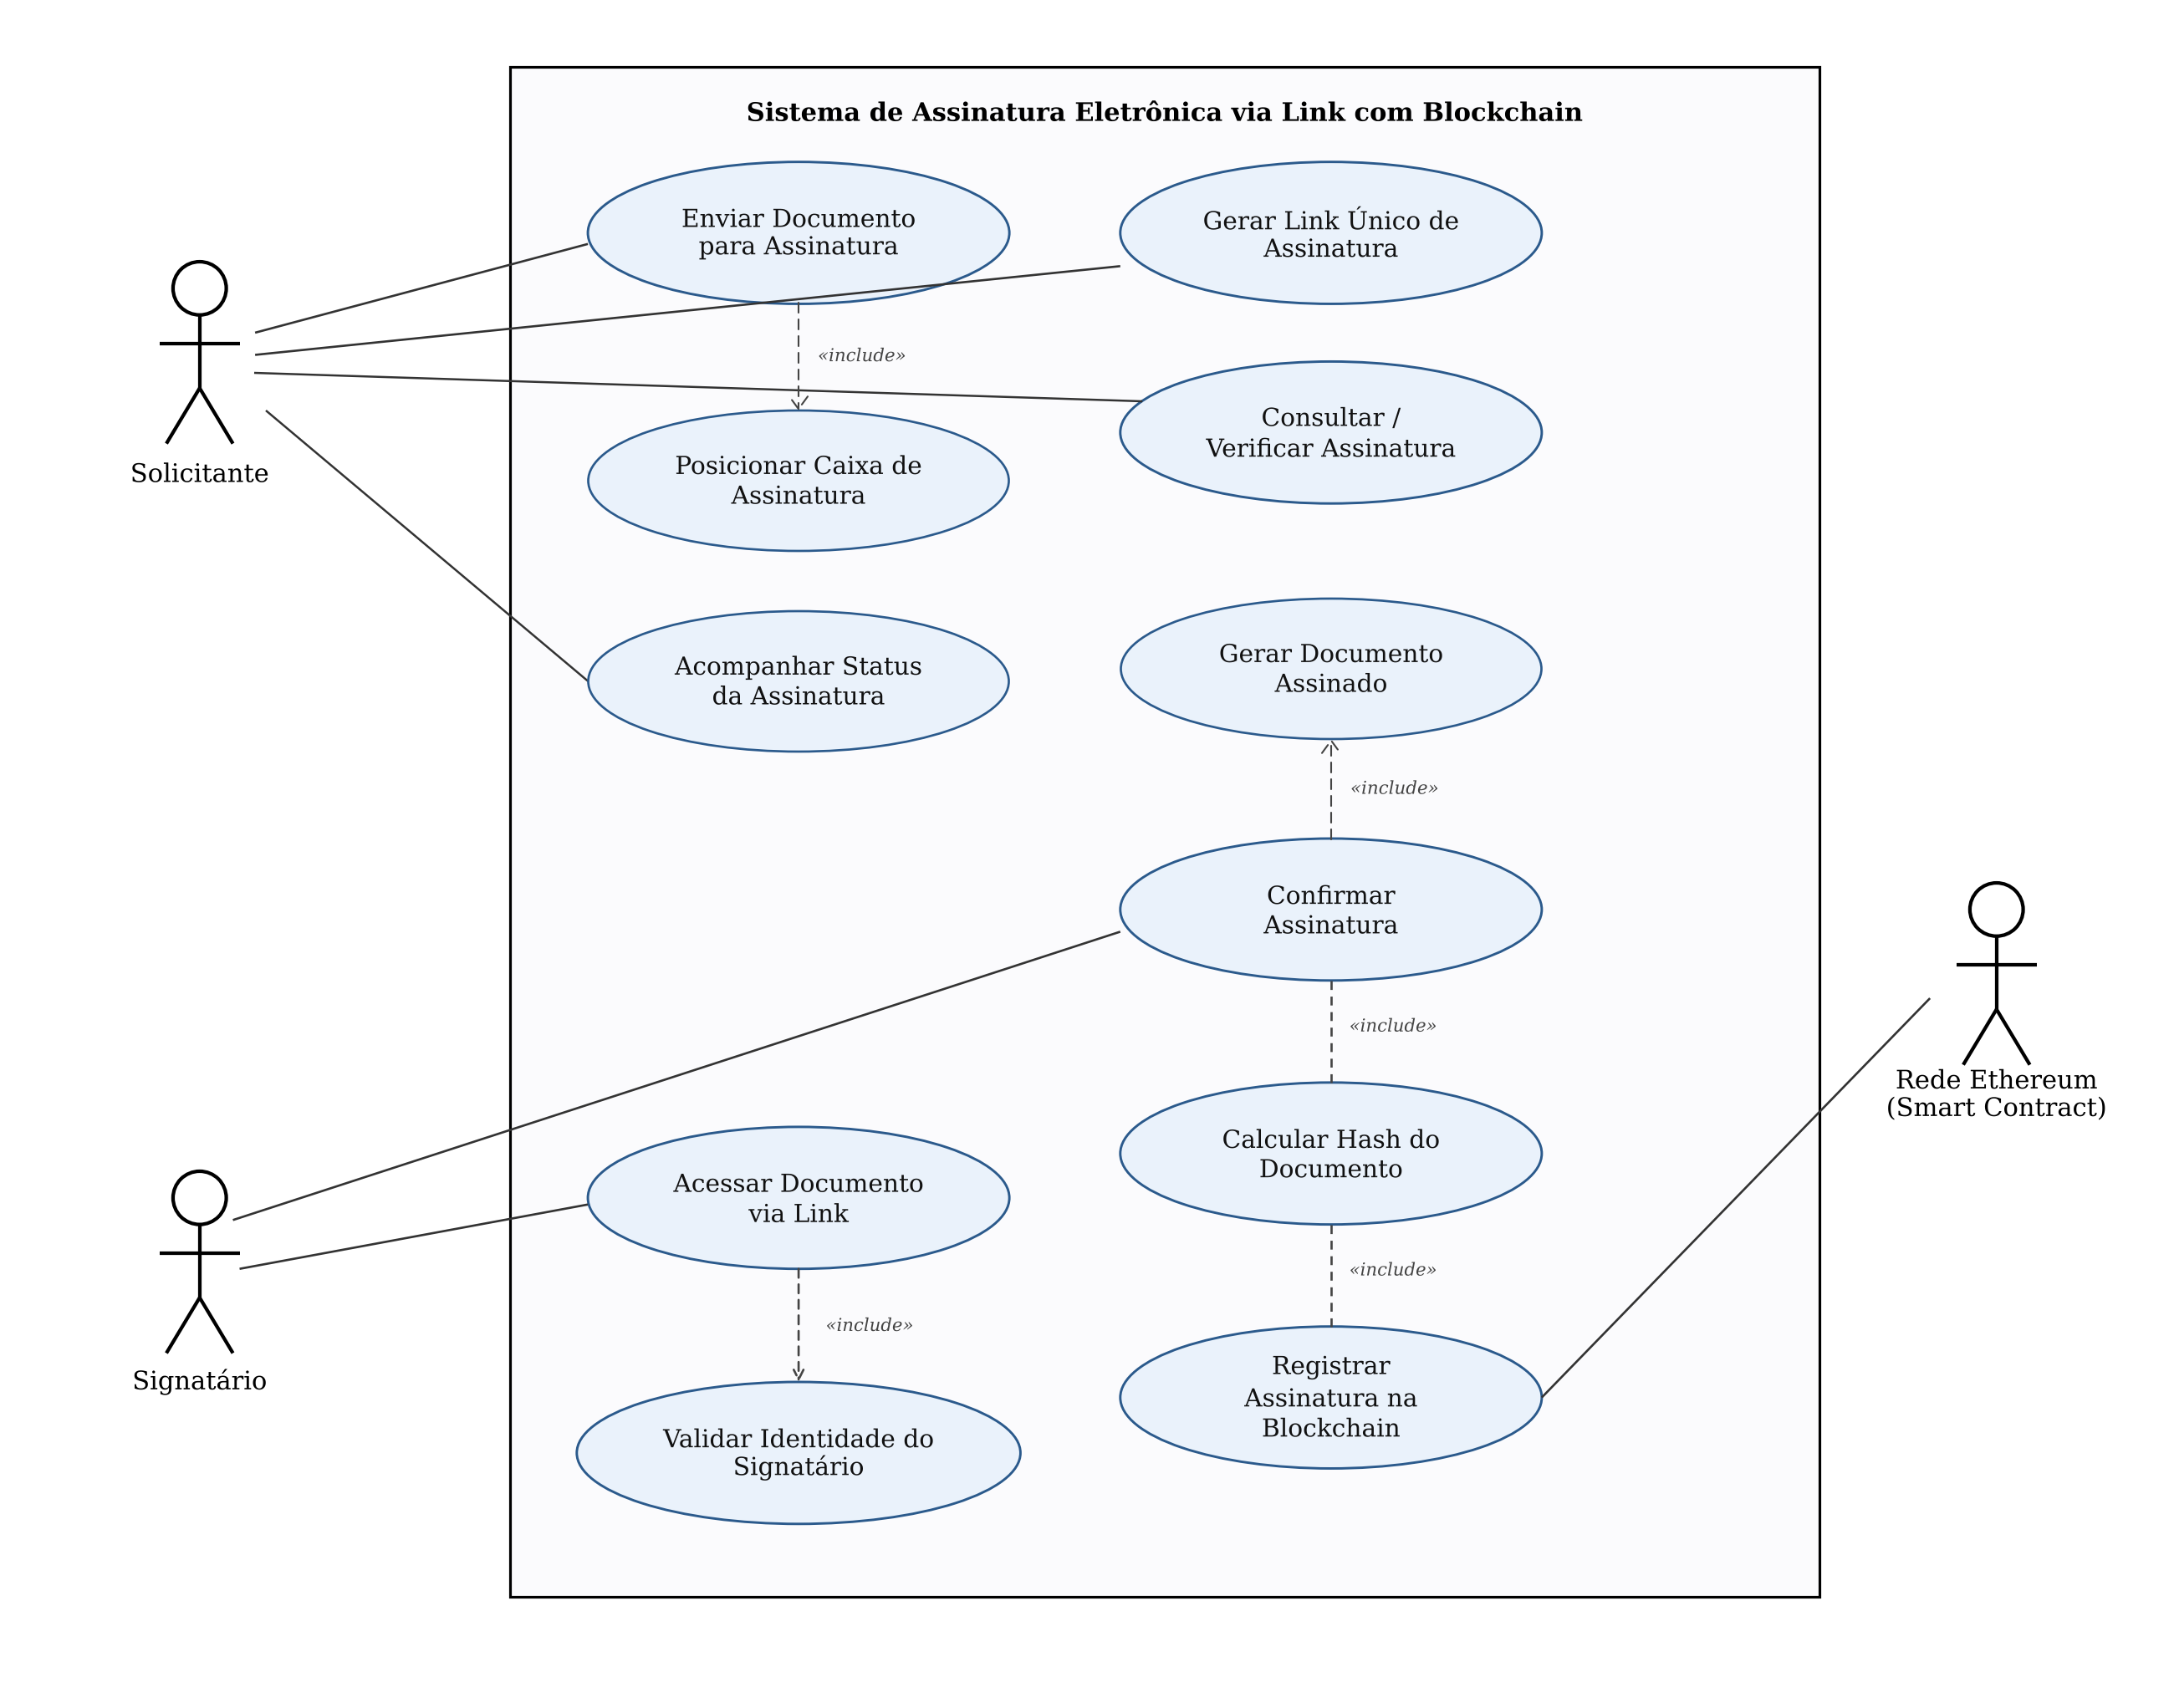
\includegraphics[width=0.9\textwidth]{diagrama_de_casos_de_uso.png}
    \legend{Fonte: elaborado pelo autor.}
\end{figure}
\FloatBarrier

\subsection{Diagrama de Atividades}
\label{sec:atividades}

O diagrama de atividades, apresentado na Figura~\ref{fig:atividades}, detalha o fluxo processual completo do sistema proposto, desde o upload do documento pelo \elem{Solicitante} até a notificação de conclusão da assinatura, indicando, junto a cada atividade, o responsável por sua execução, \elem{Solicitante}, \elem{Sistema} ou \elem{Signatário}, bem como os pontos de decisão críticos que determinam os desfechos possíveis do processo.

O fluxo tem início quando o \elem{Solicitante} realiza o upload do documento a ser assinado e informa o CPF e a data de nascimento do signatário. Essa atividade, de responsabilidade exclusiva do \elem{Solicitante}, representa o ponto de entrada do processo e corresponde, na arquitetura do sistema, à \elem{Interface do remetente} representada no diagrama de blocos da Figura~\ref{fig:arquitetura}. Na mesma interface, o \elem{Solicitante} posiciona a caixa de assinatura sobre o documento, definindo a página e o local em que a assinatura será inserida. Em seguida, o \elem{Sistema} calcula o hash criptográfico do documento original com o algoritmo SHA-256 e o armazena, preservando a impressão digital do arquivo no momento do envio. Na sequência, gera o link único de assinatura associado ao documento e o envia ao signatário, automatizando a distribuição do documento sem a necessidade de canais externos de comunicação.

Ao acessar o link, o \elem{Signatário} informa seu CPF e sua data de nascimento, e o \elem{Sistema} os confere com os dados cadastrados no upload, no primeiro ponto de decisão do fluxo. Se os dados coincidirem, o documento é aberto e o \elem{Signatário} passa à sua visualização. Se divergirem, um segundo ponto de decisão verifica se ainda restam tentativas: em caso afirmativo, o fluxo retorna, como nova tentativa, à atividade de informar os dados; caso contrário, após três tentativas sem sucesso, o \elem{Sistema} registra a falha de identificação, bloqueia o link e notifica o solicitante, encerrando o fluxo nesse ramo sem que o documento tenha sido exibido.

Após visualizar o documento, o \elem{Signatário} é confrontado com o terceiro ponto de decisão do fluxo: a confirmação da assinatura. Esse \emph{gateway} de decisão contempla dois desfechos possíveis. Caso o signatário recuse a assinatura, o sistema registra a recusa, altera o status da solicitação para recusado, invalida o link para novos acessos e notifica o solicitante, encerrando o fluxo nesse ramo. Como o registro na blockchain ocorre somente após a assinatura, nenhuma transação é enviada à rede quando há recusa. Caso a assinatura seja confirmada, o fluxo prossegue para a etapa criptográfica central do sistema.

Confirmada a assinatura, o fluxo chega ao quarto ponto de decisão, a verificação de integridade: o \elem{Sistema} recalcula o hash SHA-256 do documento e o compara com o hash armazenado no upload, mecanismo amplamente reconhecido na literatura como garantia de integridade e detecção de adulteração de dados, conforme discutido por \citeonline{stallings2017}. Se os hashes divergirem, o documento foi alterado após o envio, e o sistema bloqueia a assinatura e notifica a divergência ao solicitante, encerrando o fluxo nesse ramo. Se forem idênticos, o sistema gera uma cópia do documento com a caixa de assinatura preenchida com o nome do signatário, a data e a hora e o código de verificação, sem alterar o documento original, e coleta as evidências da assinatura, compostas pela confirmação da identidade por CPF e data de nascimento, pelo endereço IP, pela data e hora, pela identificação do navegador, pelo aceite explícito do signatário e pelo hash da cópia gerada.

Em seguida, o hash do documento e o hash das evidências são registrados no smart contract implantado na rede Ethereum, em um único registro por documento. Os dados pessoais que compõem as evidências não são enviados à rede, apenas o seu resumo criptográfico. Essa etapa materializa, no fluxo processual, os princípios de imutabilidade e descentralização descritos por \citeonline{nakamoto2008} e formalizados na arquitetura de contratos inteligentes por \citeonline{buterin2014} e \citeonline{szabo1997}.

Um quinto \emph{gateway} de decisão avalia se a transação foi efetivamente confirmada na rede blockchain. Esse ponto de verificação é metodologicamente relevante, pois reflete o tempo de confirmação variável inerente a redes blockchain públicas, aspecto discutido por \citeonline{zheng2018} e por \citeonline{alharby2017} ao tratarem dos desafios de desempenho e confiabilidade em sistemas baseados em blockchain. Caso a transação não seja confirmada, o sistema distingue duas situações. Diante de uma falha transitória, como a não inclusão da transação em um bloco dentro do prazo esperado, em razão do congestionamento da rede, ou a indisponibilidade momentânea do provedor de acesso à rede, o sistema reenvia a transação com taxa ajustada, até completar três tentativas de envio. O reenvio utiliza o mesmo número de sequência da transação original, o \emph{nonce}, de modo que a nova transação substitua a anterior em vez de gerar um segundo registro, e é precedido de uma consulta ao contrato inteligente para verificar se o hash já foi registrado, o que torna a operação idempotente. Diante de uma falha determinística, como a reversão da transação pelo contrato ou o saldo insuficiente na carteira da plataforma, repetir a operação não alteraria o resultado, e o sistema registra a falha e notifica o erro ao solicitante imediatamente. O mesmo ocorre quando as três tentativas se esgotam sem confirmação. No diagrama, essa distinção corresponde a um sexto ponto de decisão, que verifica se a falha é transitória e se ainda restam tentativas: em caso afirmativo, a atividade de reenvio da transação devolve o fluxo à verificação de confirmação na rede; caso contrário, o fluxo segue para o registro da falha. Esse tratamento evita que o status da assinatura permaneça indefinido em caso de instabilidade da rede, sem descartar registros que seriam concluídos com uma nova tentativa.

\begin{figure}[htbp]
    \centering
    \caption{Diagrama de Atividades}
    \label{fig:atividades}
    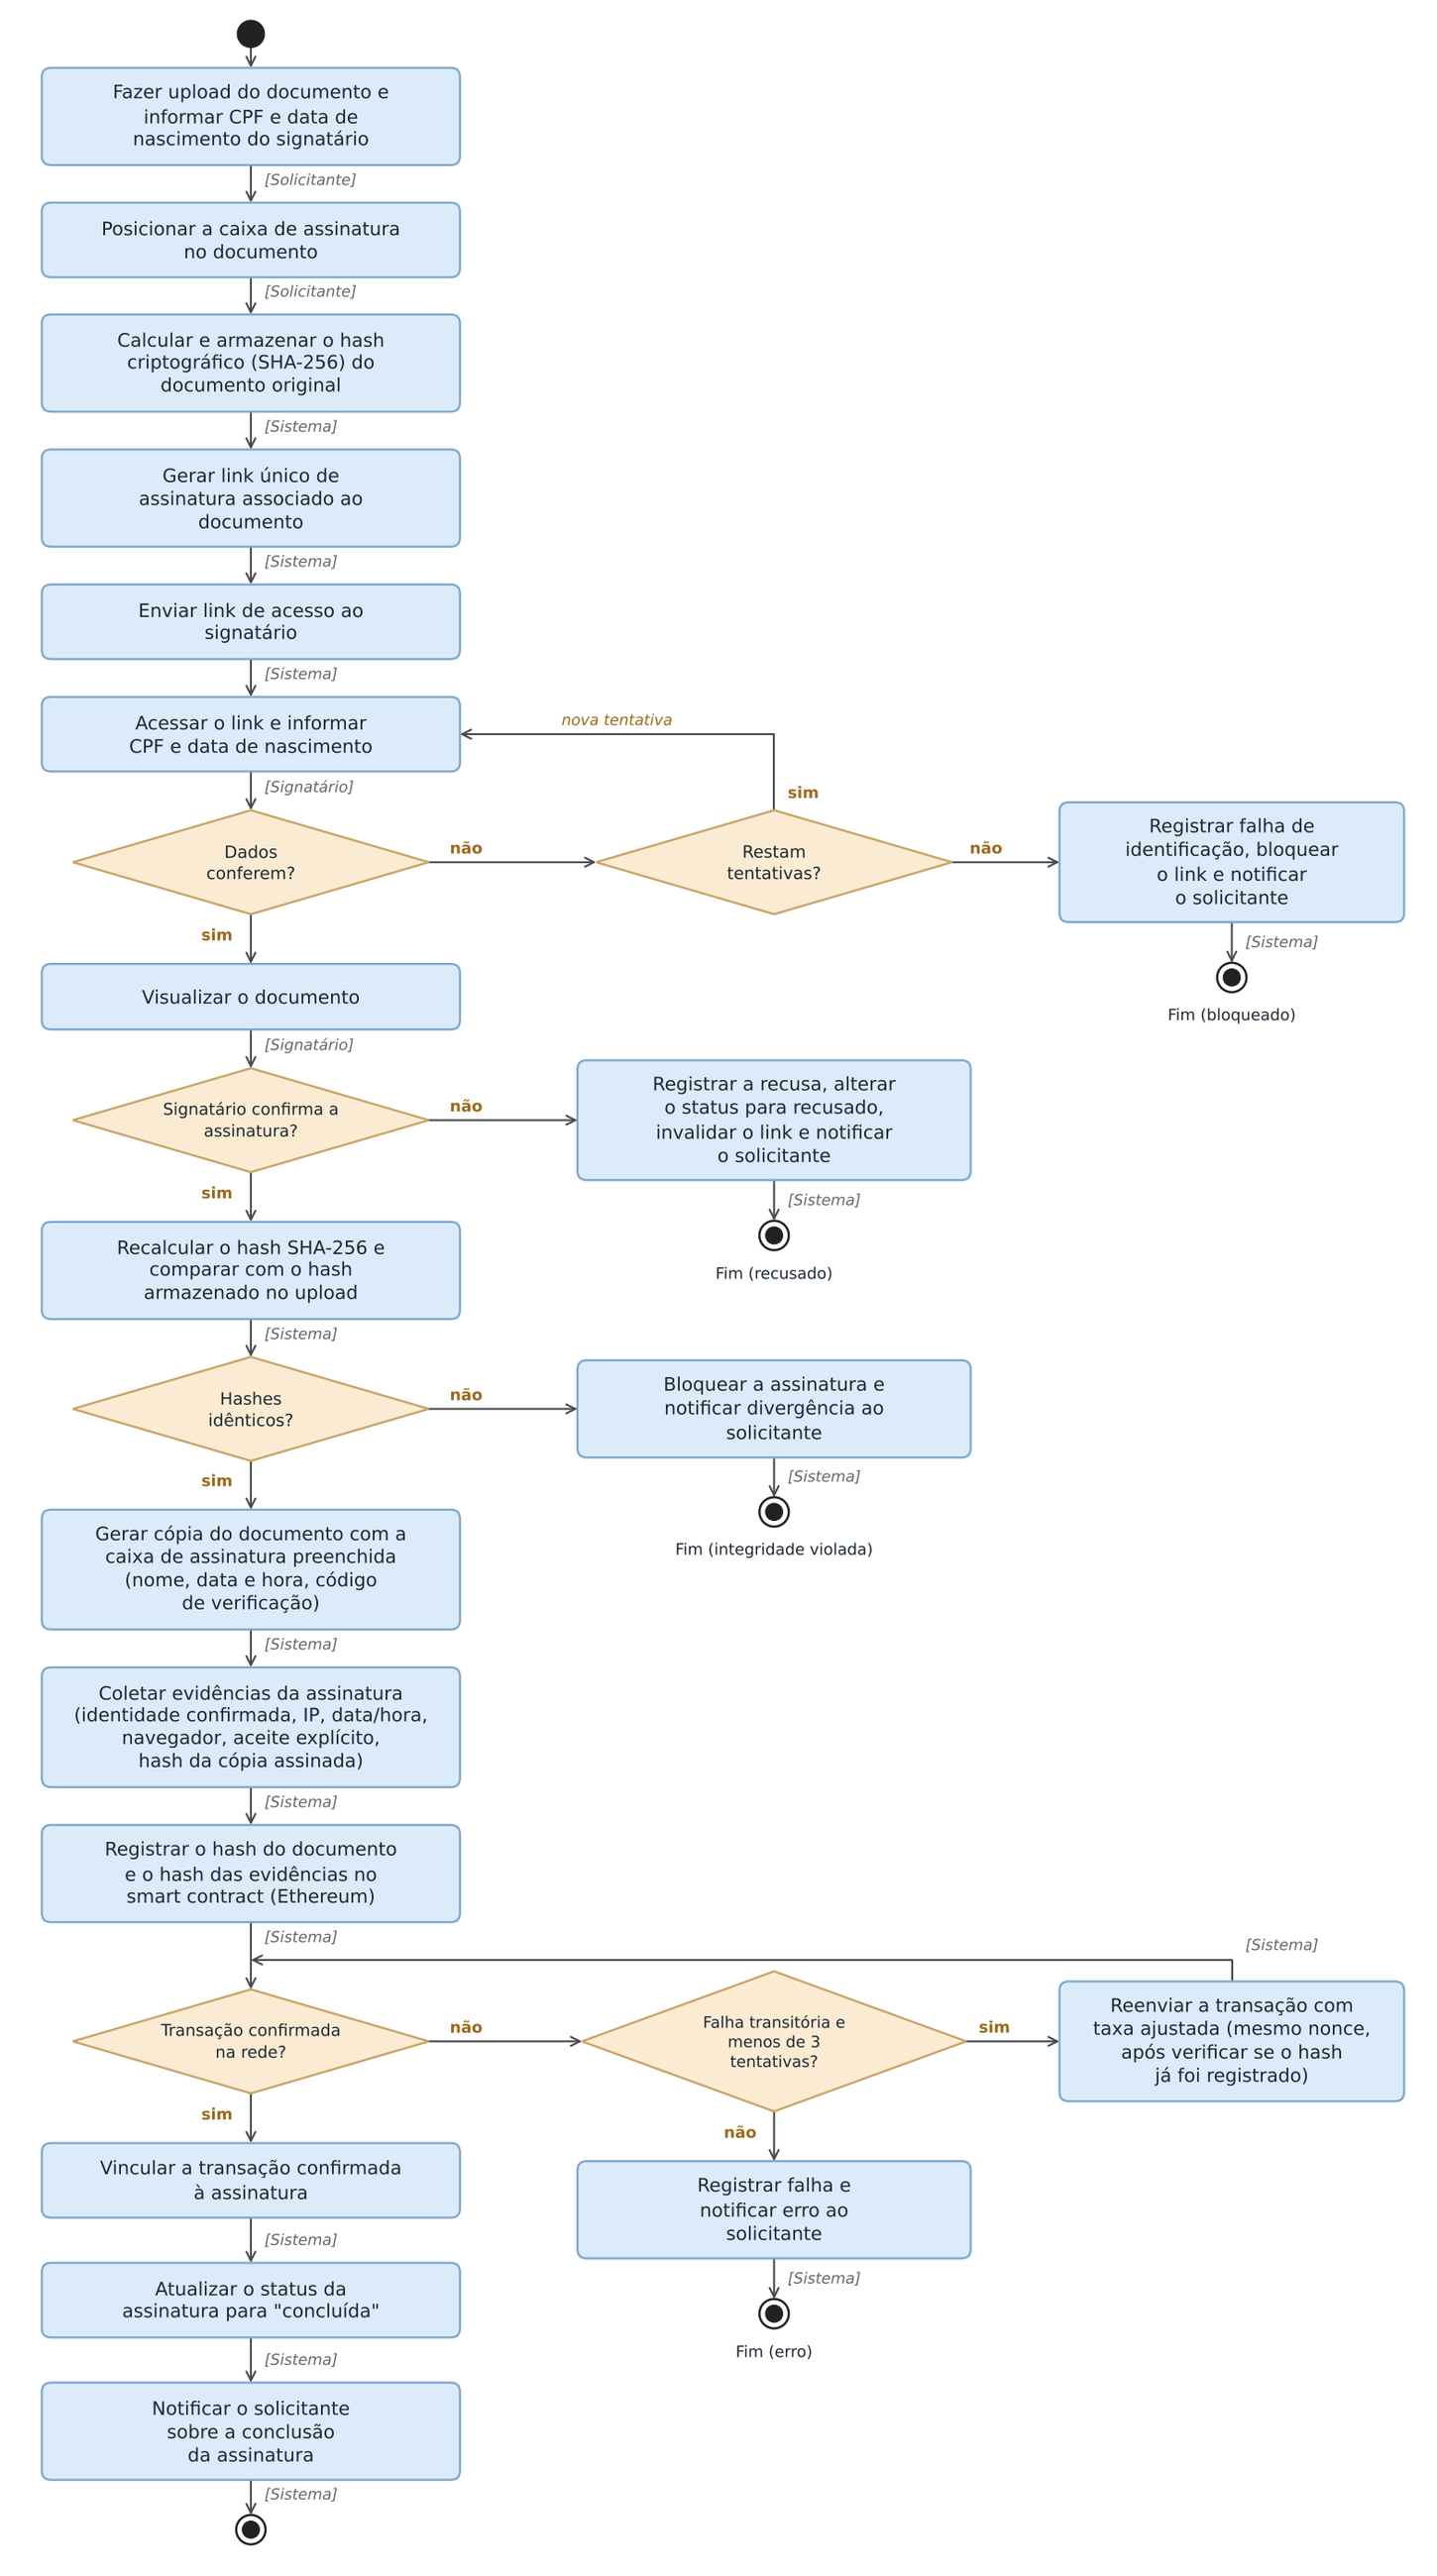
\includegraphics[width=\textwidth,height=0.80\textheight,keepaspectratio]{diagrama_de_atividades.png}
    \legend{Fonte: elaborado pelo autor.}
\end{figure}
\FloatBarrier

Confirmada a transação, o sistema vincula a transação confirmada à assinatura, etapa que consolida formalmente o vínculo entre o documento, o hash calculado e o registro na blockchain, e, em seguida, atualiza o status da assinatura para ``concluída''. O processo é finalizado com a notificação ao solicitante sobre a conclusão da assinatura, fechando o ciclo iniciado no upload do documento.

A estrutura do diagrama, com seis pontos de decisão distintos, referentes à conferência dos dados de identificação, à disponibilidade de nova tentativa de identificação, à confirmação do signatário, à integridade do documento, à confirmação da transação na rede e à possibilidade de reenvio da transação, reflete uma abordagem de tratamento de exceções que distingue claramente entre a falha de identificação do signatário, a recusa humana do processo de assinatura, a adulteração do documento e a falha técnica de infraestrutura descentralizada, distinção relevante do ponto de vista jurídico, uma vez que a validade da assinatura eletrônica, conforme a MP nº 2.200-2/2001 e a Lei nº 14.063/2020, depende tanto da manifestação inequívoca de vontade do signatário quanto da integridade técnica do registro que a comprova.

\subsection{Diagrama de Classes}
\label{sec:classes}

O diagrama de classes, apresentado na Figura~\ref{fig:classes}, modela a estrutura estática do sistema, evidenciando as entidades de domínio e seus relacionamentos, em conformidade com o fluxo funcional já apresentado nos diagramas de casos de uso e de atividades. A modelagem é composta por cinco classes principais (\elem{Usuário}, \elem{Documento}, \elem{LinkAssinatura}, \elem{Assinatura} e \elem{ContratoInteligente}), organizadas de modo a refletir a separação entre a \elem{Camada de aplicação} e a \elem{Camada de registro distribuído} da arquitetura apresentada na Figura~\ref{fig:arquitetura}.

A classe \elem{Usuário} representa tanto o solicitante quanto o signatário do processo, distinção operacionalizada por um atributo que diferencia os dois papéis sem exigir subclasses especializadas, já que essa diferenciação funcional é tratada nos casos de uso correspondentes. A classe guarda também o CPF e a data de nascimento do signatário, informados pelo solicitante no envio do documento e utilizados na verificação de identidade que antecede a abertura do documento. Esses dados pessoais permanecem armazenados exclusivamente na aplicação.

A classe \elem{Documento} relaciona-se ao \elem{Usuário} pela associação \elem{solicita}, indicando que um usuário pode requerer a assinatura de múltiplos documentos. Seu elemento central é o hash criptográfico do arquivo, calculado a partir do conteúdo original, mecanismo de garantia de integridade fundamentado teoricamente por \citeonline{stallings2017}, segundo o qual funções de hash unidirecionais permitem verificar a integridade de um dado sem expor seu conteúdo. A classe guarda ainda a posição da caixa de assinatura definida pelo solicitante, isto é, a página e as coordenadas e dimensões da caixa, e é responsável por gerar a cópia do documento com essa caixa preenchida, sem alterar o arquivo original.

A classe \elem{LinkAssinatura} associa-se ao \elem{Documento} pela relação \elem{gera}, de multiplicidade um para um, representando o link único gerado para cada submissão, identificado por um token de acesso, com controle de prazo de expiração e de status, que indica se o link foi apenas criado, ainda sem envio ao signatário, ou se a solicitação está pendente, assinada, recusada, expirada ou bloqueada, valores que correspondem aos estados do ciclo de vida do link descritos no Capítulo~\ref{sec:estados}. A classe também concentra a recusa explícita da assinatura, que encerra a solicitação sem originar uma assinatura, e a contagem das tentativas de verificação de identidade, cujo esgotamento, após três tentativas sem sucesso, bloqueia o link. Esses mecanismos conferem segurança temporal e de acesso ao processo, mitigando riscos de uso indevido de links não utilizados dentro do prazo estabelecido e de abertura do documento por terceiros.

A classe \elem{Assinatura} constitui o núcleo transacional do modelo, associando-se ao \elem{Usuário} pela relação \elem{realiza (signatário)} e ao \elem{LinkAssinatura} pela relação \elem{origina}. Nesta última, cada link origina no máximo uma assinatura, uma vez que os desfechos de recusa, de bloqueio por falha de identificação e de expiração encerram a solicitação sem gerar assinatura. Na classe convergem o hash do documento assinado, as evidências coletadas no momento da assinatura, isto é, a confirmação da identidade por CPF e data de nascimento, a data e a hora, o endereço IP, o navegador utilizado e o aceite explícito do signatário, o hash dessas evidências, a cópia do documento com a caixa de assinatura preenchida e o hash dessa cópia, que também integra as evidências, o identificador da transação registrada na rede Ethereum e a situação desse registro na blockchain, vinculando formalmente o documento à sua prova de registro na blockchain, relação que materializa os princípios de \emph{timestamping} digital estabelecidos por \citeonline{haber1991} e \citeonline{bayer1993}.

A classe \elem{ContratoInteligente}, estereotipada como smart contract em Solidity, representa a fronteira entre a aplicação e a rede blockchain, relacionando-se à \elem{Assinatura} pela associação \elem{registra via}. Ela recebe o hash do documento e o hash das evidências para registro e permite a consulta posterior desse registro. Ela operacionaliza os conceitos de contratos autoexecutáveis propostos por \citeonline{szabo1997} e implementados na plataforma Ethereum por \citeonline{buterin2014}, cuja arquitetura permite a execução determinística de lógica de negócio sobre uma estrutura de dados distribuída, princípio que remonta ao modelo de registro descentralizado introduzido por \citeonline{nakamoto2008}.

\begin{figure}[htb]
    \centering
    \caption{Diagrama de Classes}
    \label{fig:classes}
    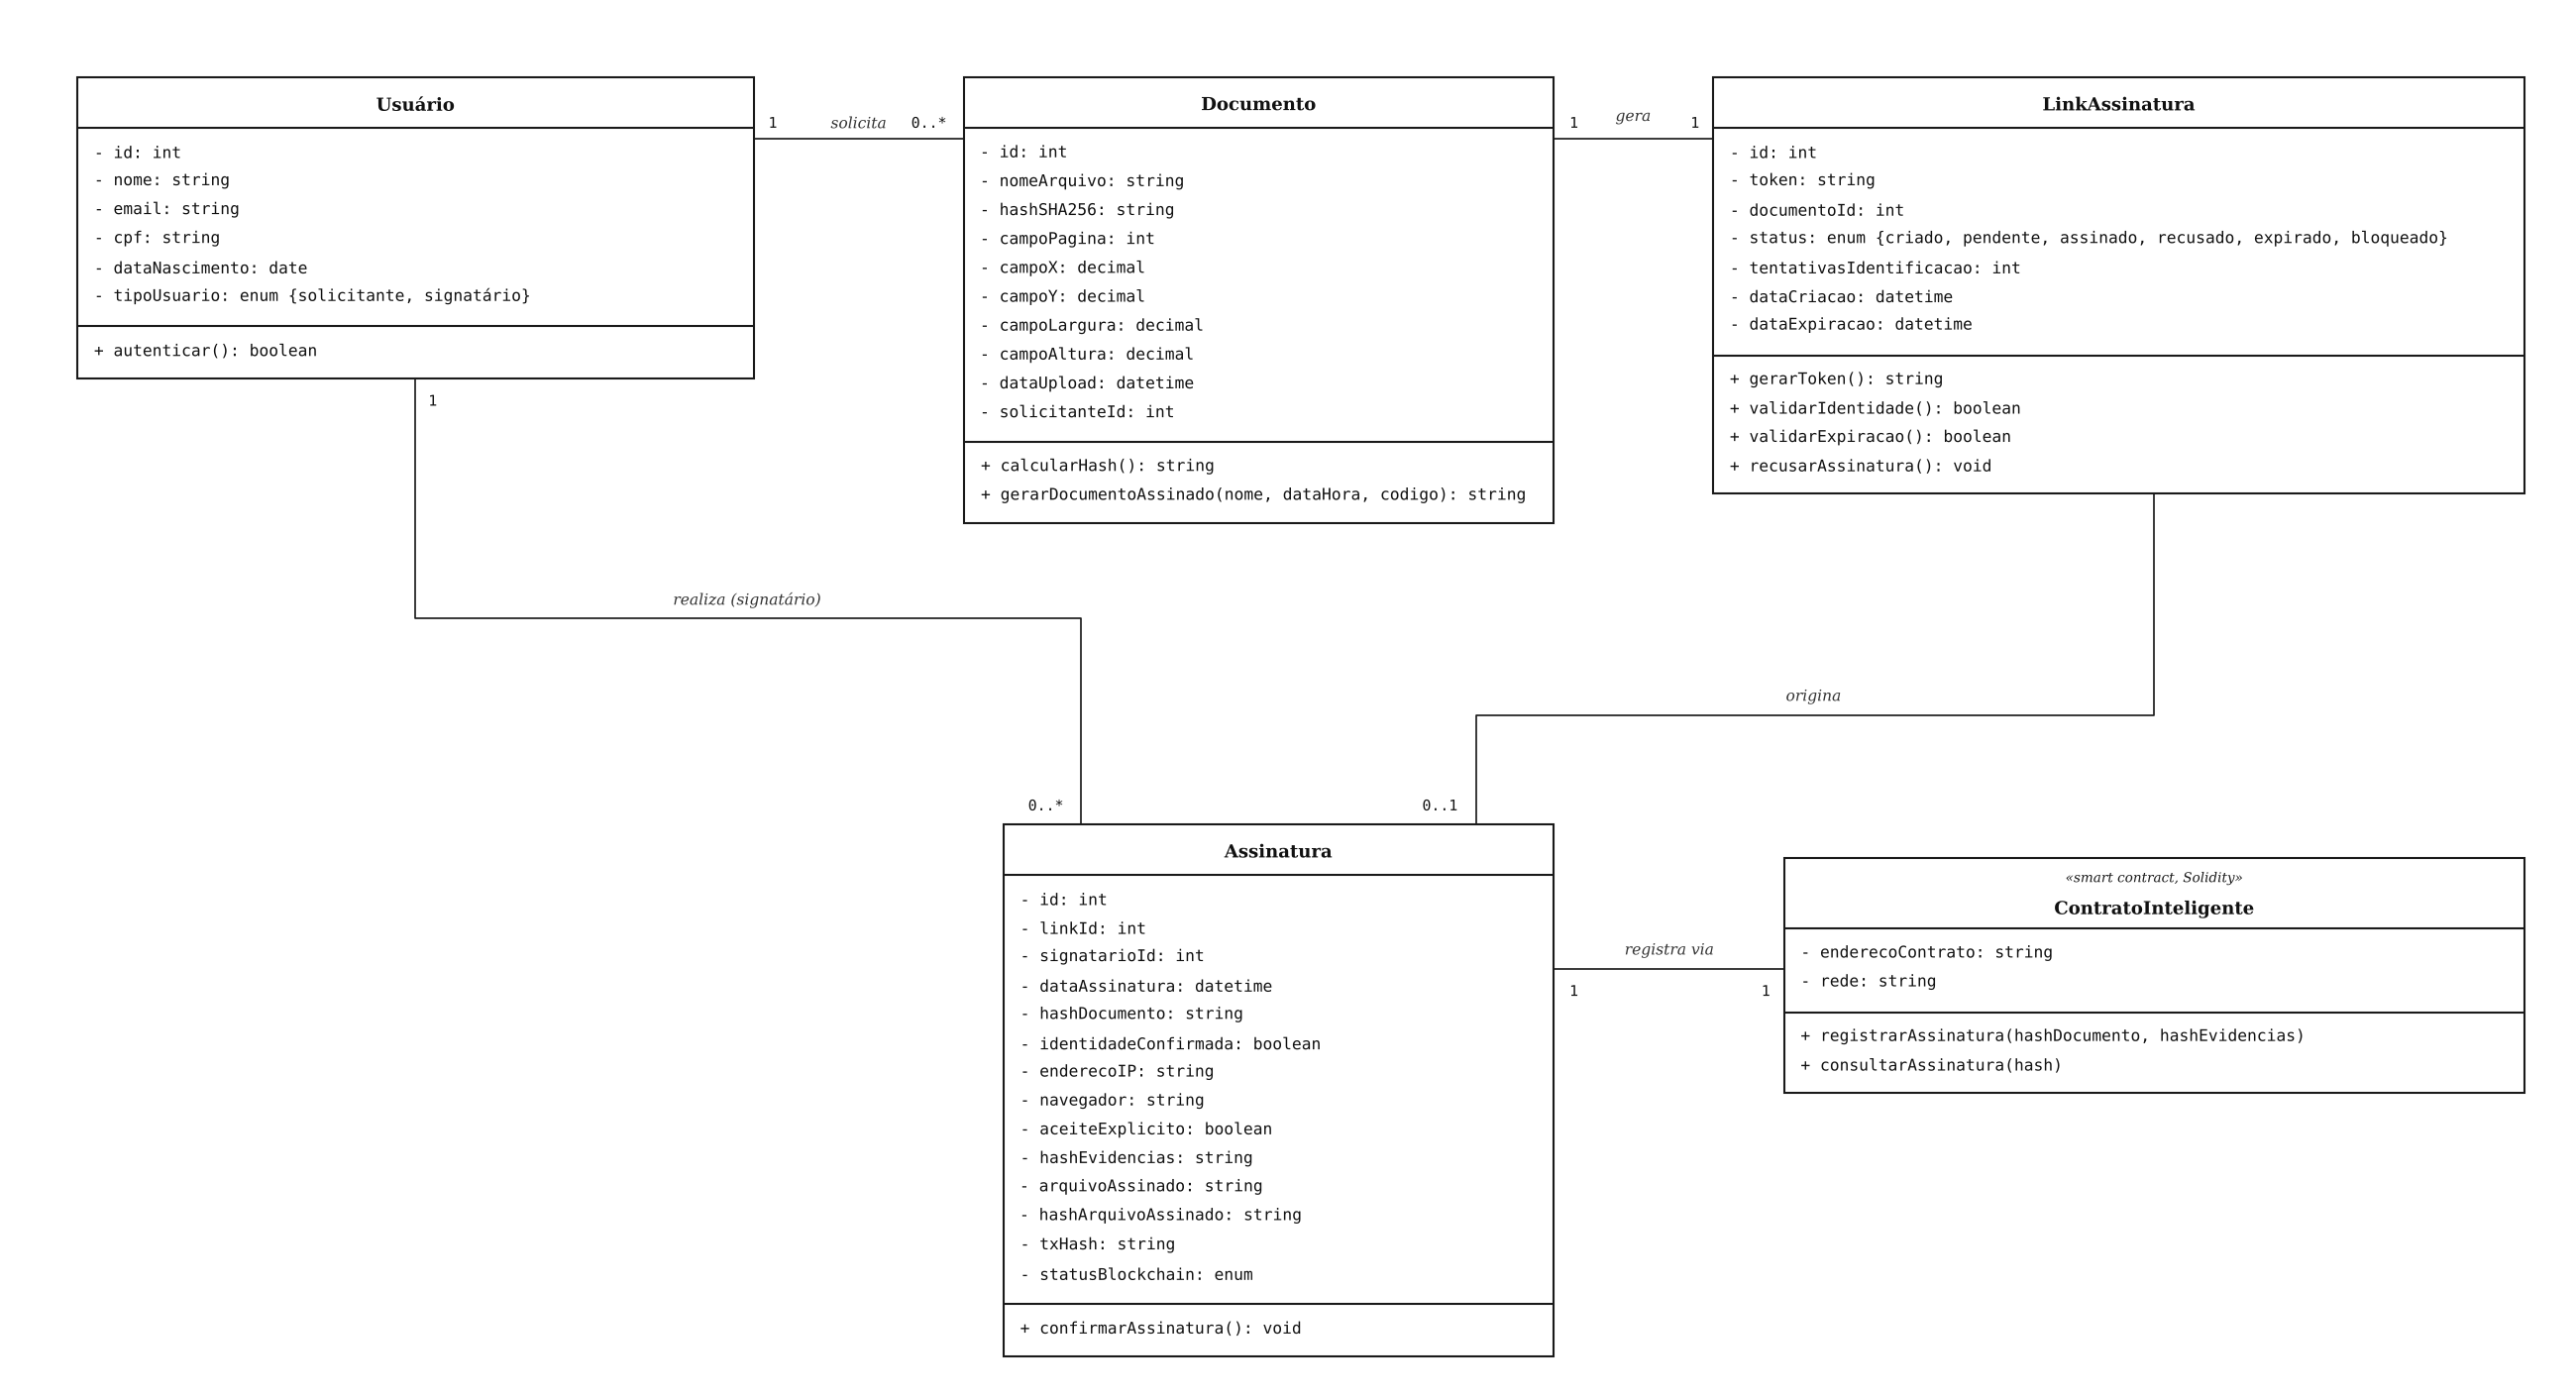
\includegraphics[width=\textwidth]{diagrama_de_classes.png}
    \legend{Fonte: elaborado pelo autor.}
\end{figure}
\FloatBarrier

Do ponto de vista metodológico, a separação entre a classe \elem{Assinatura}, pertencente ao domínio da aplicação, e a classe \elem{ContratoInteligente}, pertencente à \elem{Camada de registro distribuído}, reflete a arquitetura híbrida adotada no sistema: dados sensíveis permanecem sob custódia convencional, enquanto apenas os elementos criptográficos essenciais trafegam para a infraestrutura descentralizada. Essa opção atende tanto a requisitos de desempenho, considerando os desafios de escalabilidade discutidos por \citeonline{zheng2018} e \citeonline{alharby2017}, quanto a requisitos de conformidade legal, uma vez que a Lei nº 14.063/2020 e a MP nº 2.200-2/2001 exigem identificação inequívoca do signatário e integridade do documento assinado.

\subsection{Diagrama de Sequência}
\label{sec:sequencia}

O diagrama de sequência, apresentado na Figura~\ref{fig:sequencia}, detalha a dimensão temporal e colaborativa do processo de assinatura eletrônica, complementando os diagramas de casos de uso, de atividades e de classes ao evidenciar a ordem exata das mensagens trocadas entre os participantes no cenário de sucesso da confirmação de assinatura: o \elem{Signatário}, a \elem{Interface Web}, o \elem{Sistema}, responsável pelo processamento no \emph{backend}, e os objetos \elem{:Documento}, \elem{:Assinatura} e \elem{:ContratoInteligente}.

O cenário representado parte do momento em que o signatário já teve sua identidade confirmada pelo CPF e pela data de nascimento e visualizou o documento, etapa anterior descrita no diagrama de atividades da Figura~\ref{fig:atividades}. O processo tem início quando o \elem{Signatário} confirma a assinatura na \elem{Interface Web}, manifestando seu aceite explícito (mensagem 1), e a interface repassa a confirmação ao \elem{Sistema} (mensagem 2). A barra de ativação do \elem{Sistema}, mantida ao longo de praticamente toda a sequência, evidencia que esse componente atua como orquestrador central do processo, coordenando as chamadas aos demais objetos.

Em seguida, o \elem{Sistema} solicita ao objeto \elem{:Documento} o cálculo do hash SHA-256 do arquivo apresentado ao signatário (mensagens 3 e 4) e o compara com o hash armazenado no momento do upload (mensagem 5). Essa verificação materializa, no nível de colaboração entre objetos, o mecanismo de integridade documental fundamentado por \citeonline{stallings2017}. Conforme indica a nota associada a essa comparação, se os valores divergirem, o documento foi alterado após o envio e a assinatura é bloqueada, desfecho tratado como fluxo alternativo no diagrama de atividades da Figura~\ref{fig:atividades}. O cálculo e a comparação ocorrem inteiramente na \elem{Camada de aplicação}, antes de qualquer comunicação com a rede blockchain, o que mantém o conteúdo do documento fora da infraestrutura descentralizada.

Confirmada a integridade, o \elem{Sistema} solicita ao objeto \elem{:Documento} a geração da cópia do documento com a caixa de assinatura preenchida com o nome do signatário, a data e a hora e o código de verificação, e recebe essa cópia com o respectivo hash (mensagens 6 e 7). O documento original não é alterado, de modo que seu hash continua sendo o que será registrado na blockchain.

Em seguida, o \elem{Sistema} registra no objeto \elem{:Assinatura} as evidências coletadas, compostas pela confirmação da identidade por CPF e data de nascimento, pelo endereço IP, pela data e hora, pela identificação do navegador, pelo aceite explícito e pelo hash da cópia gerada, e recebe o hash dessas evidências (mensagens 8 e 9). Os dados pessoais permanecem armazenados na aplicação, e apenas o seu resumo criptográfico segue para a etapa seguinte.

\begin{landscape}
\begin{figure}[htbp]
    \centering
    \caption{Diagrama de Sequência}
    \label{fig:sequencia}
    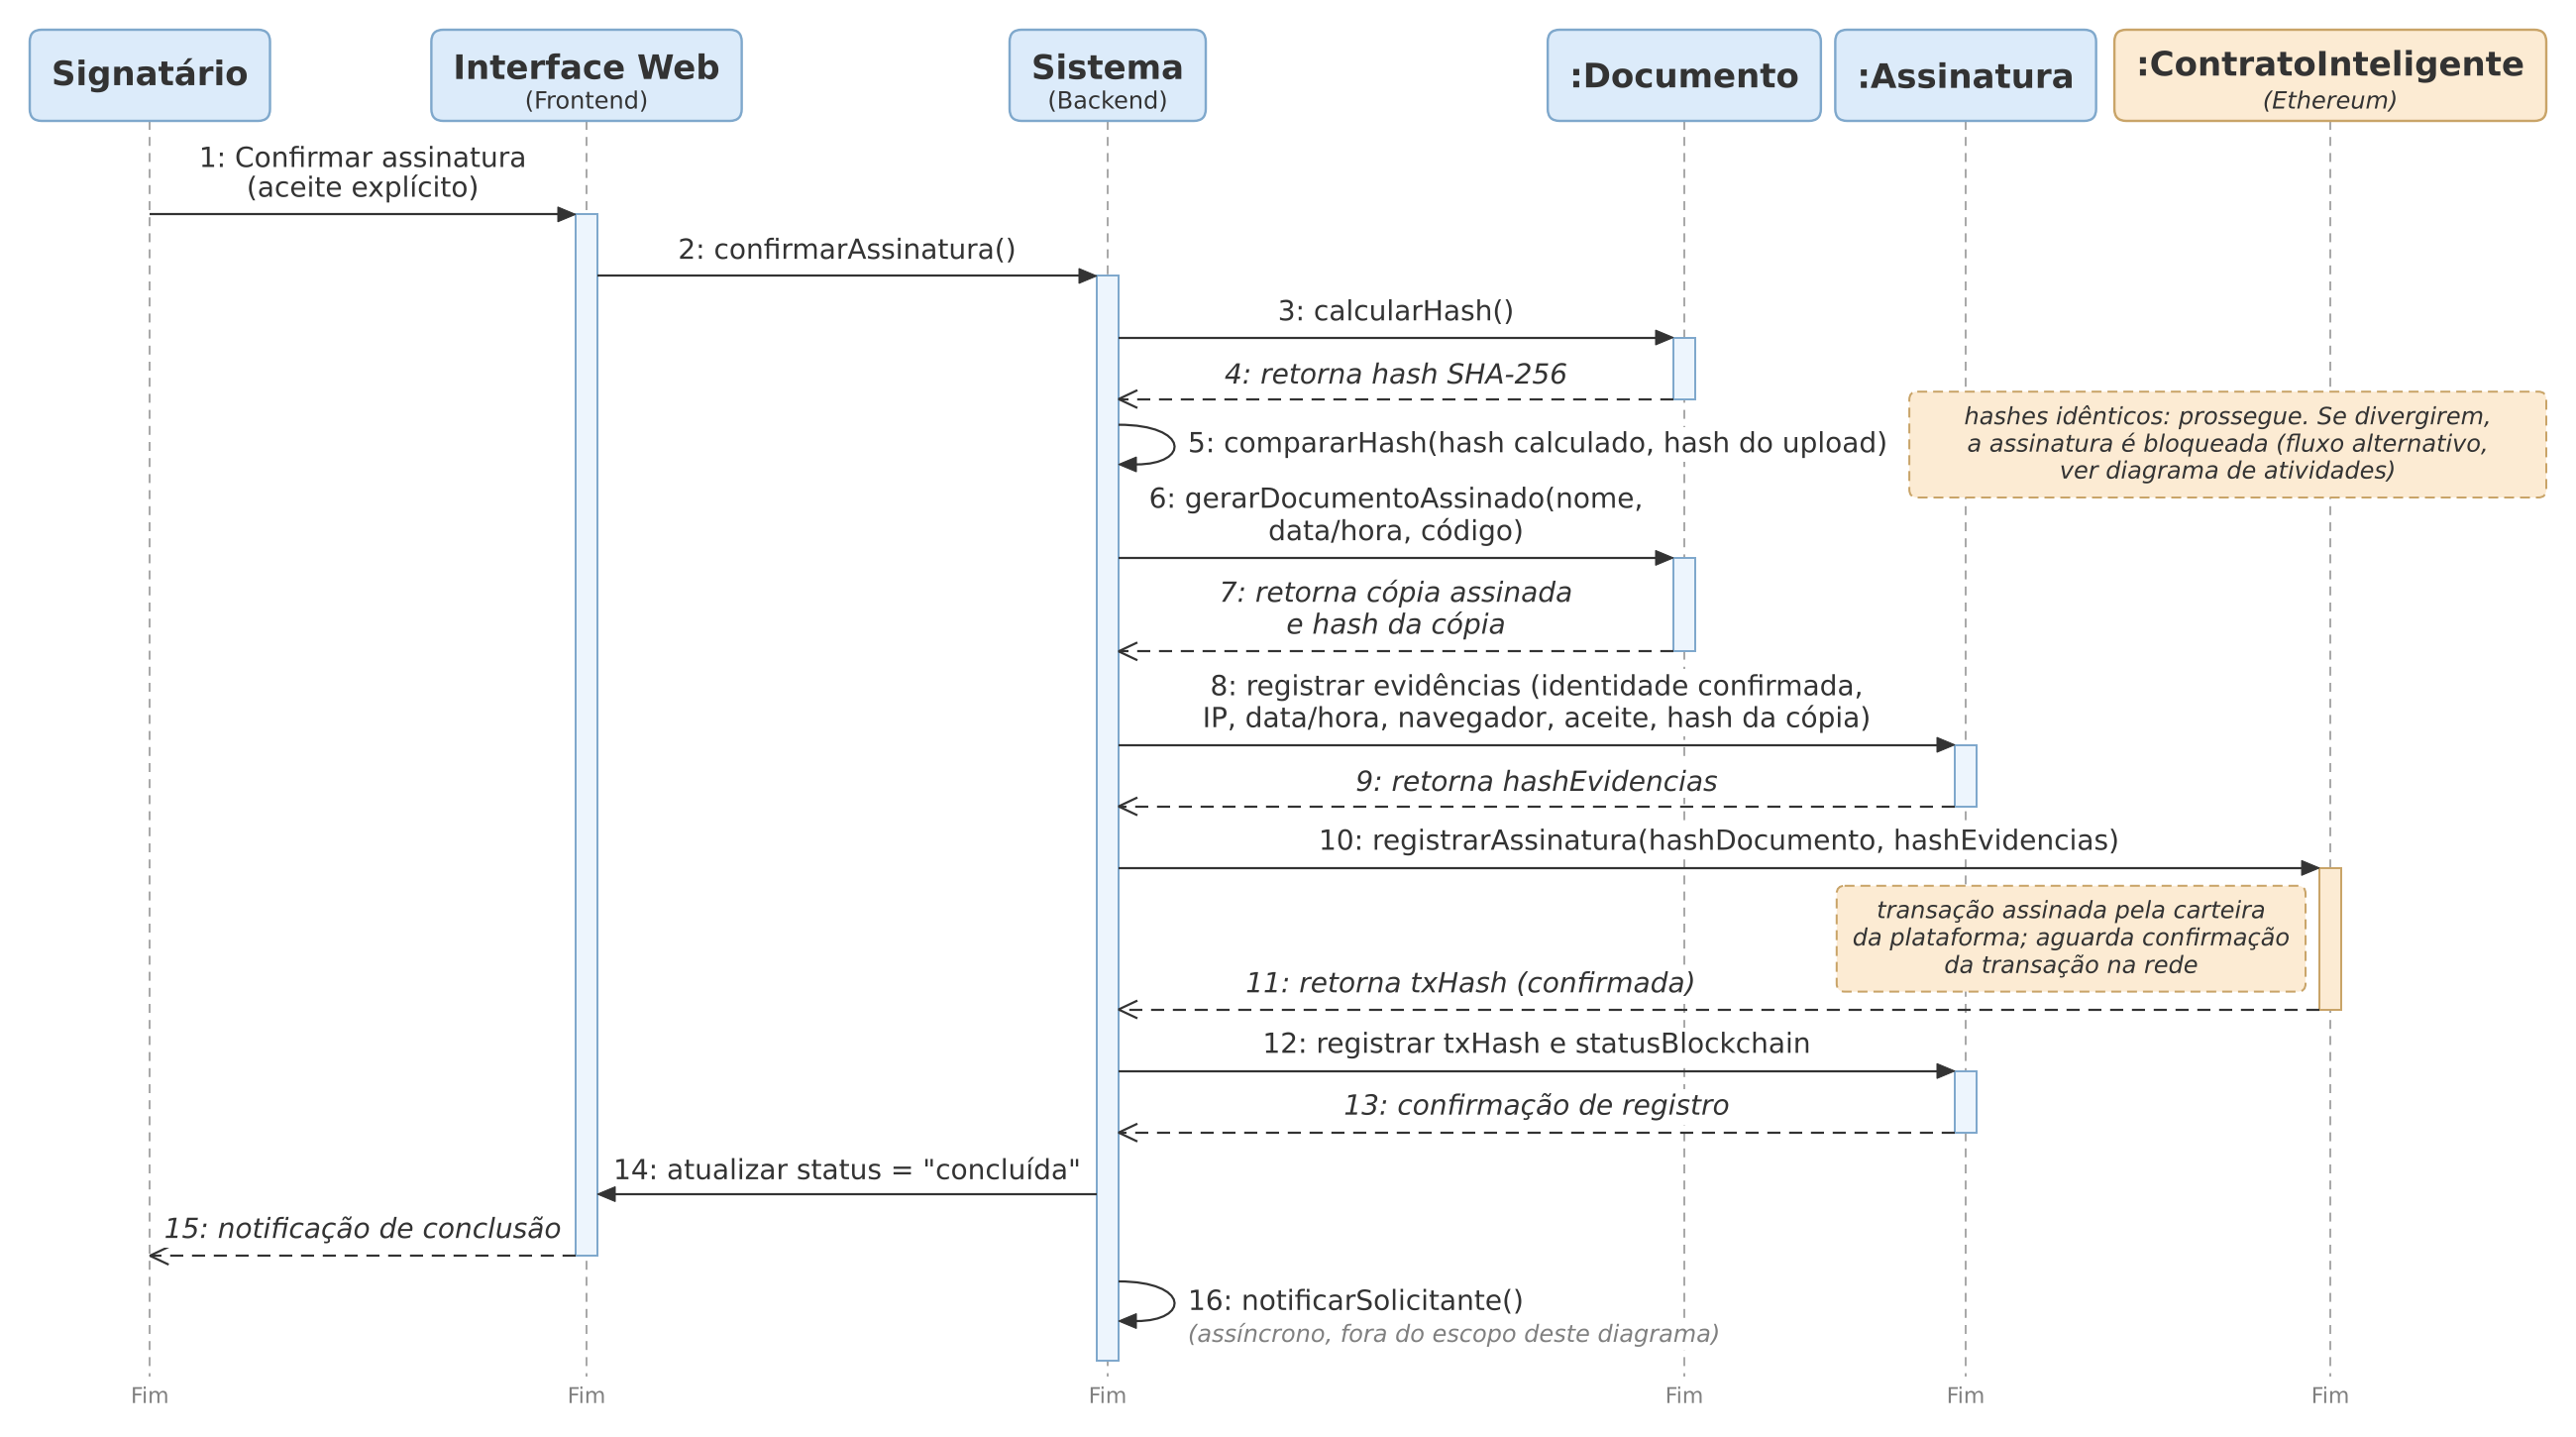
\includegraphics[width=\linewidth,height=0.88\textheight,keepaspectratio]{diagrama_de_sequencia.png}
    \legend{Fonte: elaborado pelo autor.}
\end{figure}
\end{landscape}
\FloatBarrier

O \elem{Sistema} envia então ao objeto \elem{:ContratoInteligente} o hash do documento e o hash das evidências para registro na rede Ethereum (mensagem 10), por meio de uma transação assinada pela carteira da plataforma. A nota inserida junto à barra de ativação do contrato evidencia um aspecto metodologicamente relevante: a natureza não instantânea da confirmação de transações em redes blockchain públicas, discutida por \citeonline{zheng2018} e por \citeonline{alharby2017} como um dos principais desafios de desempenho e escalabilidade desse tipo de arquitetura. Apenas após esse intervalo o contrato retorna o identificador da transação confirmada (mensagem 11), o que demonstra que o fluxo da aplicação aguarda a confirmação da rede, decisão de projeto que garante consistência entre o estado da assinatura na aplicação e seu registro imutável na blockchain.

Confirmada a transação, o \elem{Sistema} registra no objeto \elem{:Assinatura} o identificador da transação e a situação do registro na blockchain (mensagens 12 e 13). Em seguida, atualiza para concluída o status exibido na \elem{Interface Web} (mensagem 14), que notifica o \elem{Signatário} sobre a conclusão do processo (mensagem 15), encerrando o ciclo iniciado pela confirmação.

A mensagem 16, representada como uma chamada reflexiva sobre a própria barra de ativação do \elem{Sistema}, indica que a notificação ao \elem{Solicitante} ocorre de forma assíncrona e não bloqueia a resposta ao \elem{Signatário}. Essa modelagem distingue dois momentos de notificação já sugeridos nos diagramas anteriores: a confirmação imediata ao signatário, que encerra sua interação com o sistema, e o aviso posterior ao solicitante, tratado como uma responsabilidade independente do fluxo principal.

A predominância de mensagens síncronas entre o \elem{Sistema} e os objetos \elem{:Documento} e \elem{:Assinatura}, contrastada com o intervalo de espera na interação com o objeto \elem{:ContratoInteligente}, evidencia visualmente a fronteira arquitetural entre a aplicação convencional e a infraestrutura blockchain descrita no Capítulo~\ref{sec:arquitetura}. Essa representação reforça, em nível de projeto detalhado, os princípios de imutabilidade e descentralização estabelecidos por \citeonline{nakamoto2008} e operacionalizados por meio de contratos inteligentes conforme \citeonline{szabo1997} e \citeonline{buterin2014}, ao mesmo tempo em que evidencia as implicações práticas de desempenho decorrentes da adoção dessa arquitetura em um sistema de assinatura eletrônica com requisitos de resposta ao usuário.

\subsection{Diagrama de Estados}
\label{sec:estados}

O diagrama de estados, apresentado na Figura~\ref{fig:estados}, complementa a modelagem comportamental do sistema ao representar, de forma independente do fluxo processual descrito no diagrama de atividades, o ciclo de vida de duas entidades centrais do domínio: o link de assinatura e o registro da assinatura na blockchain. Enquanto os diagramas de atividades e de sequência descrevem, respectivamente, o fluxo de controle do processo e a colaboração temporal entre objetos em um cenário específico, o diagrama de estados evidencia todas as condições possíveis que um objeto pode assumir ao longo de sua existência, bem como os eventos que disparam a transição entre elas, visão que decorre diretamente dos atributos enumerados já definidos no diagrama de classes.

No ciclo de vida do link de assinatura, o estado inicial é \elem{Criado}, alcançado quando o link é gerado, após o upload do documento pelo solicitante, e antes de seu envio ao signatário. A partir da geração do token de acesso e do envio do link ao signatário, o objeto transita para o estado \elem{Pendente}, no qual permanece enquanto aguarda a ação do signatário. Esse estado admite uma transição reflexiva: caso o signatário acesse o link e deixe a página sem tomar uma decisão, ou informe CPF ou data de nascimento incorretos enquanto ainda restarem tentativas, o objeto permanece em \elem{Pendente}. A partir do estado \elem{Pendente}, quatro transições mutuamente exclusivas levam a estados finais distintos: a confirmação bem-sucedida da assinatura conduz ao estado \elem{Assinado}; a recusa explícita do signatário conduz ao estado \elem{Recusado}, que encerra a solicitação e corresponde ao ramo de recusa modelado no diagrama de atividades; a terceira tentativa de identificação sem sucesso conduz ao estado \elem{Bloqueado}, que corresponde ao ramo de falha de identificação do diagrama de atividades; e o decurso do prazo de validade sem decisão conduz ao estado \elem{Expirado}. Os estados \elem{Recusado}, \elem{Bloqueado} e \elem{Expirado} são destacados em bege, conforme a nota do diagrama, por representarem estados finais de exceção. A modelagem do desfecho \elem{Expirado} é particularmente relevante, pois representa uma condição temporal que não é explicitada no diagrama de atividades, evidenciando a complementaridade entre os diagramas comportamentais adotados no trabalho.

O segundo ciclo isola o comportamento do status de registro na blockchain, iniciando no estado \elem{AguardandoRegistro}, atingido no momento em que o hash do documento e o hash das evidências são submetidos ao smart contract. Enquanto permanece nesse estado, o sistema aguarda a inclusão da transação em um bloco e sua confirmação na rede Ethereum, comportamento consistente com a espera assíncrona já evidenciada no diagrama de sequência quanto ao caráter não instantâneo da confirmação de transações em redes blockchain públicas, conforme discutido por \citeonline{zheng2018} e por \citeonline{alharby2017}. O estado admite uma transição reflexiva que representa o reenvio da transação diante de uma falha transitória, como o congestionamento da rede ou a indisponibilidade momentânea do provedor de acesso, limitado a três tentativas de envio. A partir desse estado intermediário, a confirmação da transação na rede conduz ao estado final \elem{Confirmada}, ao passo que a reversão da transação pelo contrato, ou o esgotamento das três tentativas sem confirmação, conduz ao estado final \elem{Falha}, correspondente ao tratamento de exceção já representado no diagrama de atividades como o registro de falha e a notificação de erro ao solicitante.

A justificativa metodológica para a inclusão desse diagrama reside na sua função de tornar explícitas, em um único artefato, todas as condições que um objeto pode assumir, inclusive aquelas que, nos diagramas de atividades e de sequência, aparecem apenas implicitamente ou em cenários alternativos não detalhados no fluxo principal. O estado \elem{Expirado}, por exemplo, não é contemplado no diagrama de sequência, que modela exclusivamente o cenário de sucesso, tampouco é aprofundado no diagrama de atividades, sendo formalizado apenas na presente representação.

Do ponto de vista da conformidade legal, a separação clara entre os estados \elem{Assinado}, \elem{Recusado}, \elem{Bloqueado} e \elem{Expirado} no ciclo de vida do link, assim como entre \elem{Confirmada} e \elem{Falha} no registro blockchain, também guarda relevância jurídica: a validade da assinatura eletrônica, conforme estabelecido pela MP nº 2.200-2/2001 e pela Lei nº 14.063/2020, pressupõe que o sistema seja capaz de determinar de forma inequívoca se o processo de assinatura foi efetivamente concluído e registrado, não bastando a mera tentativa de confirmação por parte do signatário. O diagrama de estados formaliza precisamente essa exigência ao definir estados finais distintos e mutuamente exclusivos para os desfechos de sucesso, de recusa, de falha de identificação e de falha do processo.

\begin{figure}[htb]
    \centering
    \caption{Diagrama de Estados}
    \label{fig:estados}
    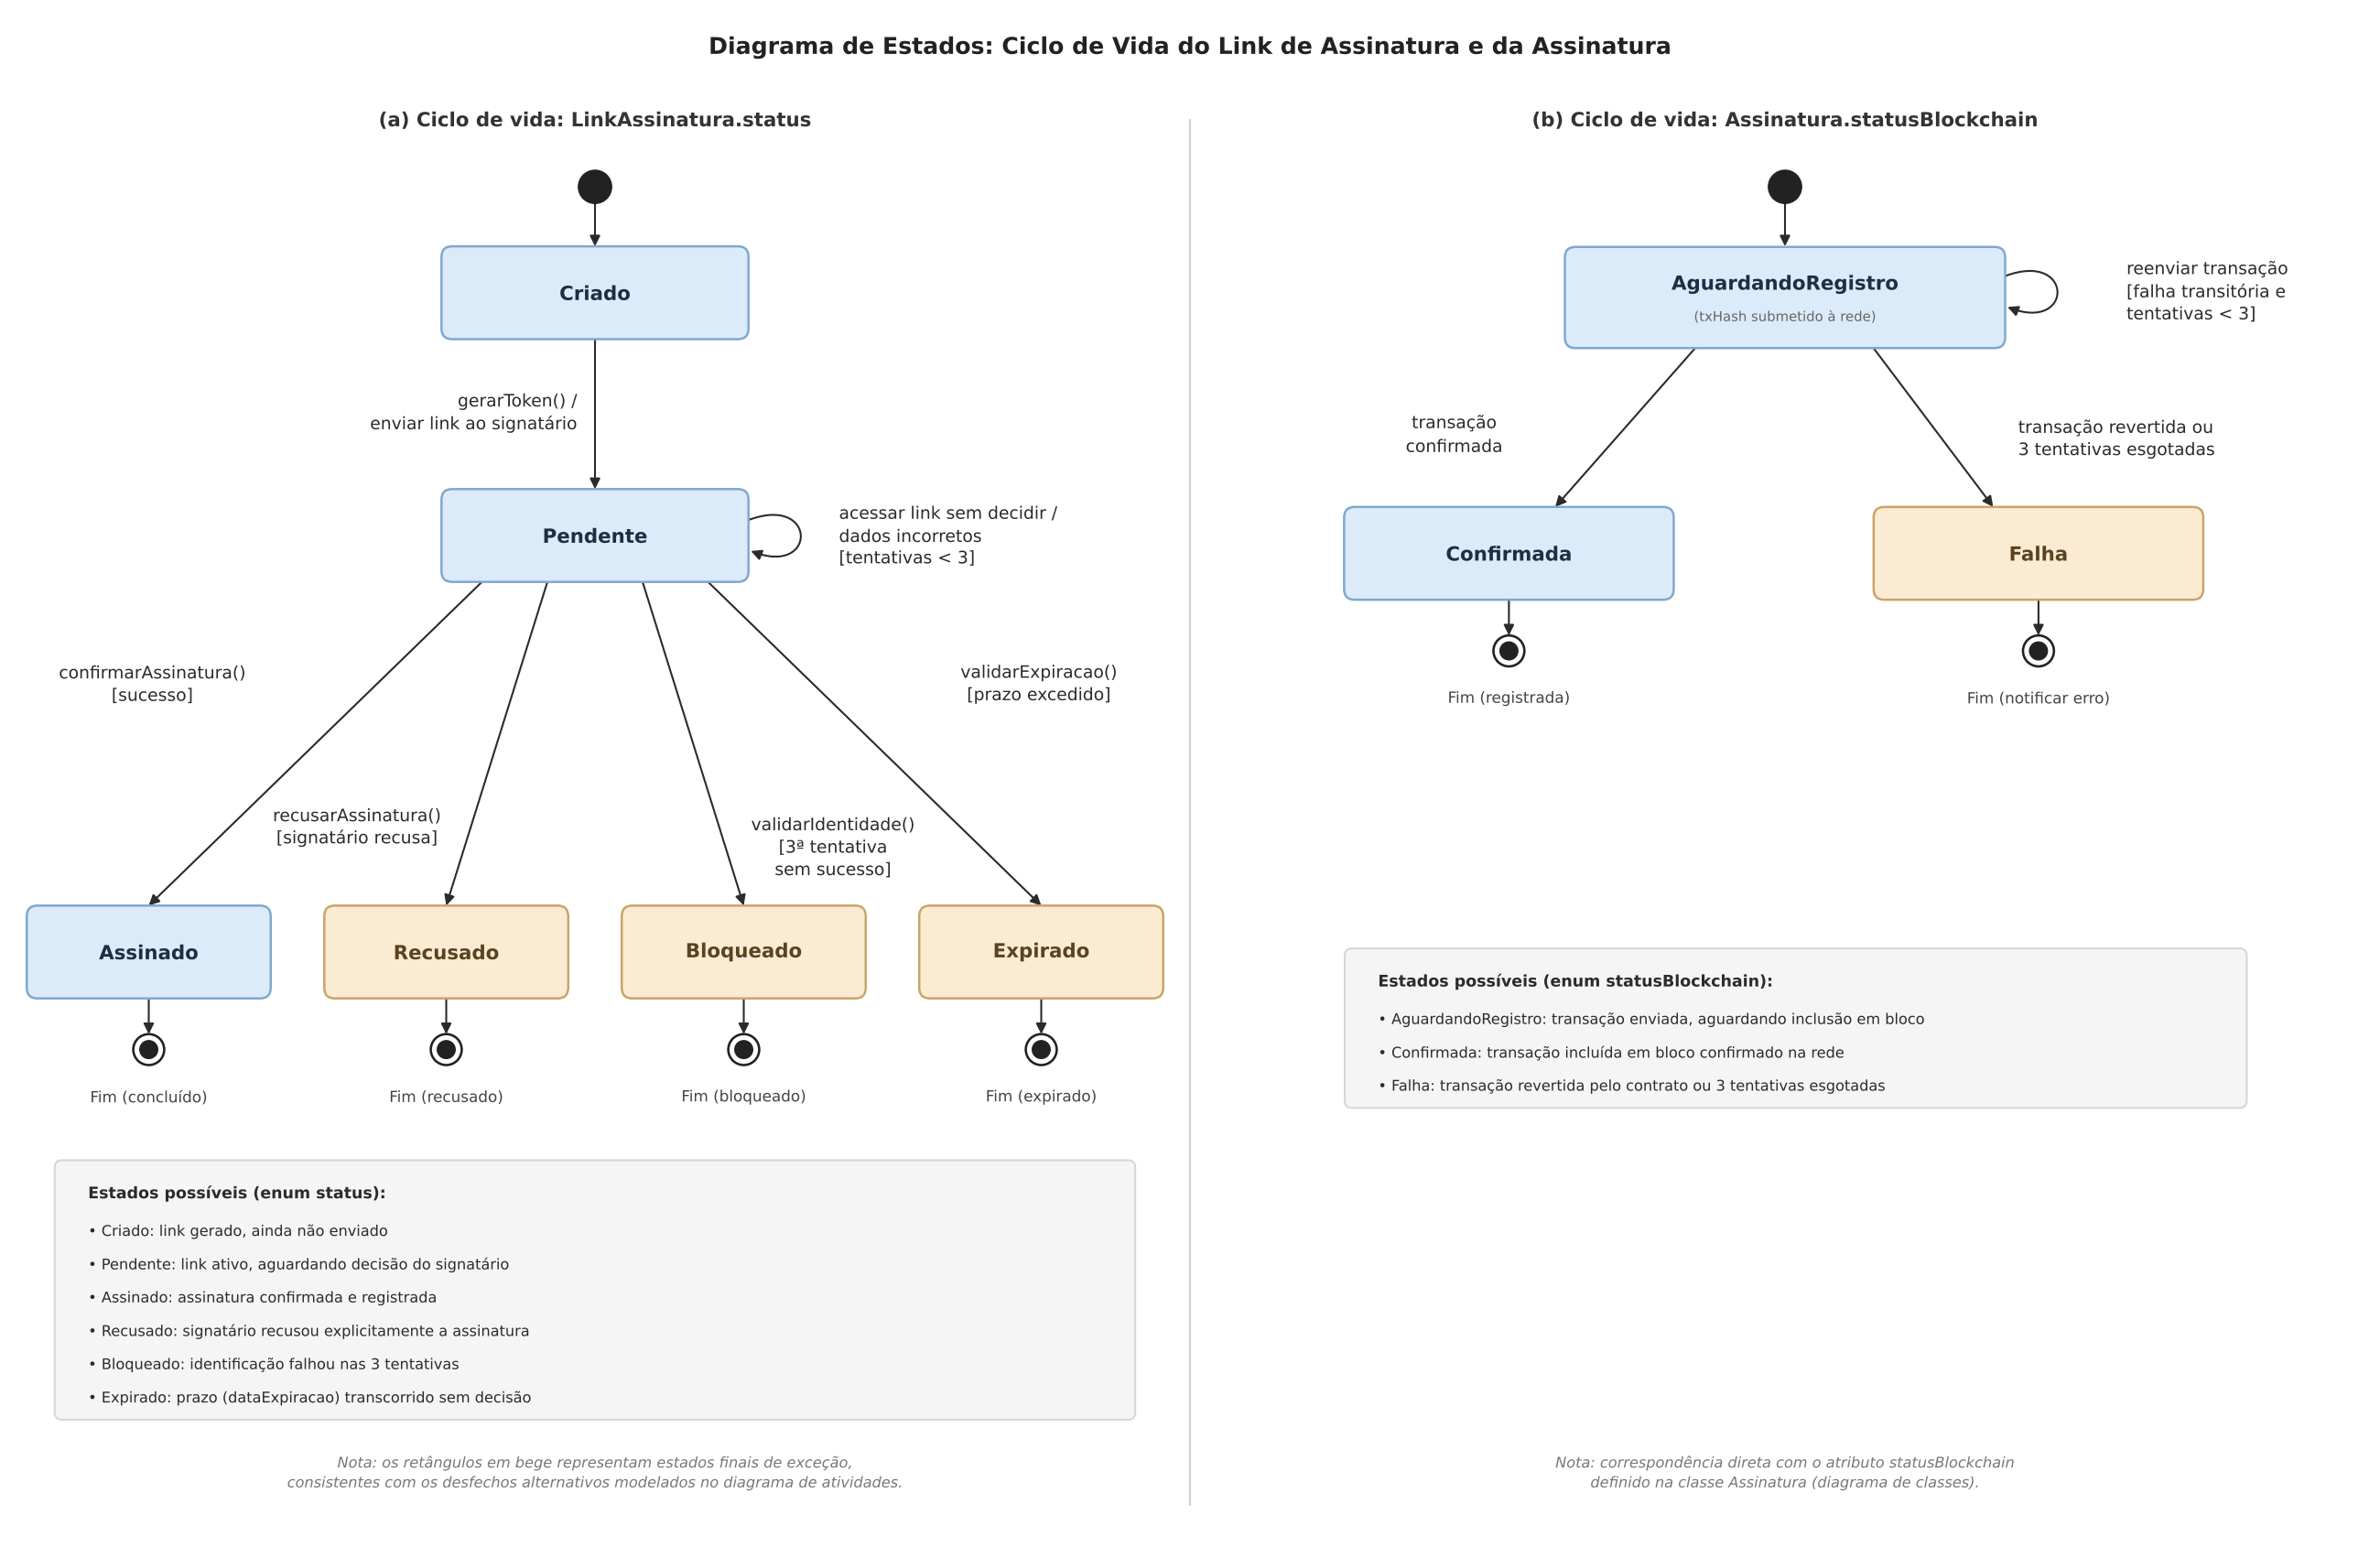
\includegraphics[width=\textwidth]{diagrama_estados.png}
    \legend{Fonte: elaborado pelo autor.}
\end{figure}
\FloatBarrier

\section{Modelagem de Banco de Dados}
\label{sec:banco}

O banco de dados relacional armazena, fora da blockchain, os dados operacionais do sistema: os usuários, os documentos enviados, os links de assinatura, as assinaturas com as respectivas evidências e a trilha de auditoria. A modelagem foi realizada no MySQL Workbench e implementada no MySQL 8.0, mantendo correspondência com as classes apresentadas no Capítulo~\ref{sec:classes}, com exceção da classe \elem{ContratoInteligente}, cujos dados residem na própria blockchain. Nenhuma das informações descritas nesta seção é enviada à rede: a blockchain recebe apenas o hash do documento e o hash das evidências.

\subsection{Modelo Conceitual (MER)}
\label{sec:mer}

O modelo entidade-relacionamento, apresentado na Figura~\ref{fig:mer}, foi obtido no MySQL Workbench a partir do banco implementado e reúne cinco entidades: \elem{usuario}, \elem{documento}, \elem{link\_assinatura}, \elem{assinatura} e \elem{log\_auditoria}. A entidade \elem{usuario} representa tanto o solicitante quanto o signatário, distinguidos por um atributo de tipo, em correspondência com a classe \elem{Usuário}.

\begin{figure}[htb]
    \centering
    \caption{Modelo entidade-relacionamento do banco de dados}
    \label{fig:mer}
    \IfFileExists{diagrama_mer.png}{%
        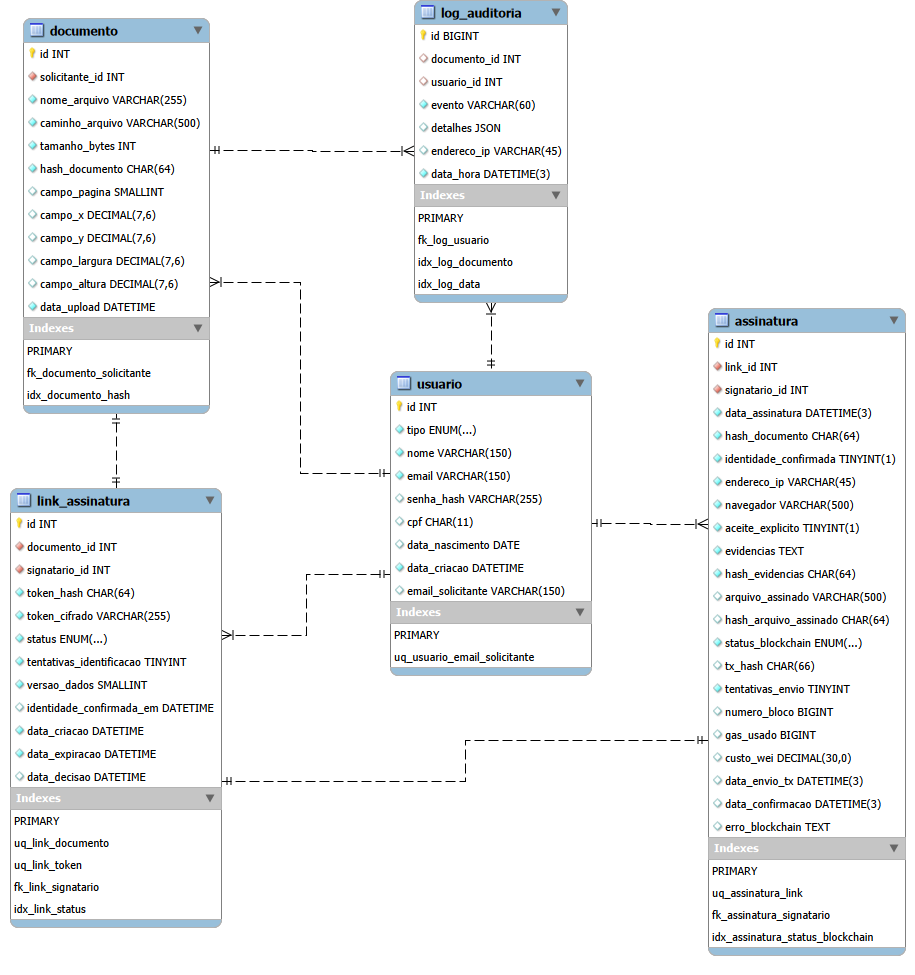
\includegraphics[width=\textwidth]{diagrama_mer.png}%
    }{%
        \fbox{\parbox{0.9\textwidth}{\centering\vspace{1cm}[VALIDAR/COMPLETAR] Inserir o diagrama exportado do MySQL Workbench, salvo como diagrama\_mer.png na pasta do TCC.\vspace{1cm}}}%
    }
    \legend{Fonte: elaborado pelo autor.}
\end{figure}
\FloatBarrier

Um usuário solicitante pode enviar vários documentos, e cada documento pertence a um único solicitante. Cada documento possui exatamente um link de assinatura, relacionamento de cardinalidade um para um, e cada link se destina a um único signatário. Um link origina no máximo uma assinatura, já que os desfechos de recusa, de bloqueio e de expiração encerram a solicitação sem gerar assinatura, e cada assinatura é realizada por um signatário. Por fim, a entidade \elem{log\_auditoria} registra os eventos do processo, cada um associado opcionalmente a um documento e a um usuário.

\subsection{Modelo Lógico}

No modelo lógico, cada entidade corresponde a uma tabela com chave primária numérica de incremento automático, e os relacionamentos são implementados pelas chaves estrangeiras apresentadas no Quadro~\ref{quadro:chaves}. Em todas elas, a alteração do identificador referenciado é propagada automaticamente. A exclusão de um usuário, documento ou link referenciado é impedida, de modo que nenhuma assinatura perca o vínculo com o documento e com o signatário, enquanto, na trilha de auditoria, a exclusão apenas anula a referência, preservando o registro do evento.

\begin{quadro}[htb]
    \caption{Chaves estrangeiras do banco de dados}
    \label{quadro:chaves}
    \centering
    \small
    \begin{tabular}{L{3.3cm}L{3.6cm}L{3.8cm}L{3.3cm}}
        \toprule
        \textbf{Tabela} & \textbf{Chave estrangeira} & \textbf{Referência} & \textbf{Na exclusão} \\
        \midrule
        \elem{documento} & \elem{solicitante\_id} & \elem{usuario.id} & Impedida \\
        \elem{link\_assinatura} & \elem{documento\_id} & \elem{documento.id} & Impedida \\
        \elem{link\_assinatura} & \elem{signatario\_id} & \elem{usuario.id} & Impedida \\
        \elem{assinatura} & \elem{link\_id} & \elem{link\_assinatura.id} & Impedida \\
        \elem{assinatura} & \elem{signatario\_id} & \elem{usuario.id} & Impedida \\
        \elem{log\_auditoria} & \elem{documento\_id} & \elem{documento.id} & Anula a referência \\
        \elem{log\_auditoria} & \elem{usuario\_id} & \elem{usuario.id} & Anula a referência \\
        \bottomrule
    \end{tabular}
    \legend{Fonte: elaborado pelo autor.}
\end{quadro}

Além das chaves, o banco aplica restrições que reforçam as regras do sistema independentemente da aplicação. As restrições de unicidade garantem um único link por documento, um token exclusivo por link, no máximo uma assinatura por link e um e-mail exclusivo entre os solicitantes, este último por meio de uma coluna calculada que contém o e-mail apenas dos usuários do tipo solicitante. As restrições de verificação exigem senha para o solicitante e CPF e data de nascimento para o signatário, e limitam a três tanto as tentativas de identificação quanto as tentativas de envio da transação, de modo que esses limites sejam respeitados mesmo diante de uma falha na aplicação.

A Figura~\ref{fig:mer} apresenta também os índices de cada tabela. Além dos índices das chaves primárias, das chaves estrangeiras e das restrições de unicidade, há índices para a busca de documentos pelo hash, de links e de assinaturas pela situação e de eventos de auditoria pela data, consultas usadas, respectivamente, na recusa do envio de um PDF duplicado, na expiração dos links, na retomada dos registros pendentes na blockchain e na consulta à trilha de auditoria.

Duas decisões de modelagem merecem destaque. A primeira é a ausência de uma tabela específica para o registro na blockchain: como há um único registro por assinatura, os dados da transação, como o identificador, o bloco, o gas consumido e a situação do registro, são armazenados na própria tabela \elem{assinatura}, em correspondência com a classe \elem{Assinatura}. A segunda é o armazenamento das evidências como texto, exatamente na forma em que foram usadas no cálculo do seu hash, o que permite recalcular esse hash e compará-lo com o valor registrado no contrato.

\subsection{Dicionário de Dados}

Os Quadros~\ref{quadro:dic-usuario} a~\ref{quadro:dic-log} descrevem os campos de cada tabela, com o tipo de dado, as restrições e a finalidade de cada um.

% Espaço menor entre os quadros do dicionário, para que dois caibam na mesma página.
\begingroup
\setlength{\intextsep}{6pt plus 2pt minus 2pt}
\begin{quadro}[H]
    \caption{Dicionário de dados da tabela usuario}
    \label{quadro:dic-usuario}
    \centering
    \footnotesize
    \begin{tabular}{L{4.5cm}L{3.6cm}L{6.3cm}}
        \toprule
        \textbf{Campo} & \textbf{Tipo e restrições} & \textbf{Descrição} \\
        \midrule
        \elem{id} & INT UNSIGNED; PK; incremento automático & Identificador do usuário \\
        \elem{tipo} & ENUM; obrigatório & Papel do usuário: solicitante ou signatário \\
        \elem{nome} & VARCHAR(150); obrigatório & Nome completo \\
        \elem{email} & VARCHAR(150); obrigatório & E-mail de acesso do solicitante ou de envio do link ao signatário \\
        \elem{senha\_hash} & VARCHAR(255); obrigatório para o solicitante & Hash bcrypt da senha do solicitante \\
        \elem{cpf} & CHAR(11); obrigatório para o signatário & CPF do signatário, somente dígitos, usado na verificação de identidade \\
        \elem{data\_nascimento} & DATE; obrigatório para o signatário & Data de nascimento do signatário, usada na verificação de identidade \\
        \elem{data\_criacao} & DATETIME; padrão: data atual & Data do cadastro \\
        \elem{email\_solicitante} & VARCHAR(150); calculado; único & E-mail apenas dos solicitantes, que garante e-mail exclusivo entre eles \\
        \bottomrule
    \end{tabular}
    \legend{Fonte: elaborado pelo autor.}
\end{quadro}

\begin{quadro}[H]
    \caption{Dicionário de dados da tabela documento}
    \label{quadro:dic-documento}
    \centering
    \footnotesize
    \begin{tabular}{L{4.5cm}L{3.6cm}L{6.3cm}}
        \toprule
        \textbf{Campo} & \textbf{Tipo e restrições} & \textbf{Descrição} \\
        \midrule
        \elem{id} & INT UNSIGNED; PK; incremento automático & Identificador do documento \\
        \elem{solicitante\_id} & INT UNSIGNED; FK; obrigatório & Solicitante que enviou o documento \\
        \elem{nome\_arquivo} & VARCHAR(255); obrigatório & Nome original do arquivo \\
        \elem{caminho\_arquivo} & VARCHAR(500); obrigatório & Local do PDF original no armazenamento do servidor \\
        \elem{tamanho\_bytes} & INT UNSIGNED; obrigatório & Tamanho do arquivo \\
        \elem{hash\_documento} & CHAR(64); obrigatório; indexado & SHA-256 do PDF original, em hexadecimal, registrado na blockchain \\
        \elem{campo\_pagina} & SMALLINT UNSIGNED; opcional & Página da caixa de assinatura, a partir de 1 \\
        \elem{campo\_x}, \elem{campo\_y} & DECIMAL(7,6); opcional & Posição do canto superior esquerdo da caixa, em frações da largura e da altura da página exibida \\
        \elem{campo\_largura}, \elem{campo\_altura} & DECIMAL(7,6); opcional & Dimensões da caixa, em frações da página \\
        \elem{data\_upload} & DATETIME; padrão: data atual & Data do envio \\
        \bottomrule
    \end{tabular}
    \legend{Fonte: elaborado pelo autor.}
\end{quadro}

\begin{quadro}[H]
    \caption{Dicionário de dados da tabela link\_assinatura}
    \label{quadro:dic-link}
    \centering
    \footnotesize
    \begin{tabular}{L{4.5cm}L{3.6cm}L{6.3cm}}
        \toprule
        \textbf{Campo} & \textbf{Tipo e restrições} & \textbf{Descrição} \\
        \midrule
        \elem{id} & INT UNSIGNED; PK; incremento automático & Identificador do link \\
        \elem{documento\_id} & INT UNSIGNED; FK; único & Documento do link, um por documento \\
        \elem{signatario\_id} & INT UNSIGNED; FK; obrigatório & Signatário a quem o link se destina \\
        \elem{token\_hash} & CHAR(64); único & SHA-256 do token presente na URL, usado para localizar o link \\
        \elem{token\_cifrado} & VARCHAR(255); obrigatório & Token cifrado com AES-256-GCM, cuja chave fica fora do banco, para reexibir o link ao solicitante \\
        \elem{status} & ENUM; padrão: criado & Situação do link: criado, pendente, assinado, recusado, expirado ou bloqueado \\
        \elem{tentativas\_identificacao} & TINYINT UNSIGNED; padrão: 0; no máximo 3 & Tentativas de identificação sem sucesso \\
        \elem{versao\_dados} & SMALLINT UNSIGNED; padrão: 0 & Incrementada a cada correção dos dados do signatário, invalidando identificações anteriores \\
        \elem{identidade\_confirmada\_em} & DATETIME; opcional & Data da última identificação bem-sucedida \\
        \elem{data\_criacao} & DATETIME; padrão: data atual & Data de criação do link \\
        \elem{data\_expiracao} & DATETIME; obrigatório & Fim da validade do link \\
        \elem{data\_decisao} & DATETIME; opcional & Data em que o link chegou a um estado final \\
        \bottomrule
    \end{tabular}
    \legend{Fonte: elaborado pelo autor.}
\end{quadro}

\begin{quadro}[H]
    \caption{Dicionário de dados da tabela assinatura}
    \label{quadro:dic-assinatura}
    \centering
    \footnotesize
    \begin{tabular}{L{4.5cm}L{3.6cm}L{6.3cm}}
        \toprule
        \textbf{Campo} & \textbf{Tipo e restrições} & \textbf{Descrição} \\
        \midrule
        \elem{id} & INT UNSIGNED; PK; incremento automático & Identificador da assinatura \\
        \elem{link\_id} & INT UNSIGNED; FK; único & Link que originou a assinatura, no máximo uma por link \\
        \elem{signatario\_id} & INT UNSIGNED; FK; obrigatório & Signatário que assinou \\
        \elem{data\_assinatura} & DATETIME(3); obrigatório & Data e hora da assinatura, com milissegundos \\
        \elem{hash\_documento} & CHAR(64); obrigatório & Hash do documento, conferido no momento da assinatura \\
        \elem{identidade\_confirmada} & TINYINT(1); obrigatório & Confirmação da identidade por CPF e data de nascimento \\
        \elem{endereco\_ip} & VARCHAR(45); obrigatório & Endereço IP do signatário, nas versões 4 ou 6 do protocolo \\
        \elem{navegador} & VARCHAR(500); obrigatório & Identificação do navegador utilizado \\
        \elem{aceite\_explicito} & TINYINT(1); obrigatório & Registro do aceite explícito \\
        \elem{evidencias} & TEXT; obrigatório & Evidências em JSON, exatamente como usadas no cálculo do seu hash \\
        \elem{hash\_evidencias} & CHAR(64); obrigatório & SHA-256 das evidências, registrado na blockchain \\
        \elem{arquivo\_assinado} & VARCHAR(500); opcional & Local da cópia do documento com a caixa de assinatura preenchida \\
        \elem{hash\_arquivo\_assinado} & CHAR(64); opcional & SHA-256 da cópia assinada, também incluído nas evidências \\
        \elem{status\_blockchain} & ENUM; padrão: aguardando\_registro & Situação do registro: aguardando registro, confirmada ou falha \\
        \elem{tx\_hash} & CHAR(66); opcional & Hash da transação que registrou a assinatura \\
        \elem{tentativas\_envio} & TINYINT UNSIGNED; padrão: 0; no máximo 3 & Tentativas de envio da transação \\
        \elem{numero\_bloco} & BIGINT UNSIGNED; opcional & Bloco em que a transação foi incluída \\
        \elem{gas\_usado} & BIGINT UNSIGNED; opcional & Gas consumido pela transação \\
        \elem{custo\_wei} & DECIMAL(30,0); opcional & Custo da transação em \emph{wei}, igual ao gas consumido multiplicado pelo preço efetivo \\
        \elem{data\_envio\_tx} & DATETIME(3); opcional & Primeiro envio da transação \\
        \elem{data\_confirmacao} & DATETIME(3); opcional & Confirmação da transação na rede \\
        \elem{erro\_blockchain} & TEXT; opcional & Motivo da falha no registro, quando houver \\
        \bottomrule
    \end{tabular}
    \legend{Fonte: elaborado pelo autor.}
\end{quadro}

\begin{quadro}[H]
    \caption{Dicionário de dados da tabela log\_auditoria}
    \label{quadro:dic-log}
    \centering
    \footnotesize
    \begin{tabular}{L{4.5cm}L{3.6cm}L{6.3cm}}
        \toprule
        \textbf{Campo} & \textbf{Tipo e restrições} & \textbf{Descrição} \\
        \midrule
        \elem{id} & BIGINT UNSIGNED; PK; incremento automático & Identificador do evento \\
        \elem{documento\_id} & INT UNSIGNED; FK; opcional & Documento relacionado ao evento \\
        \elem{usuario\_id} & INT UNSIGNED; FK; opcional & Usuário relacionado ao evento \\
        \elem{evento} & VARCHAR(60); obrigatório & Tipo do evento, como envio, acesso ao link, assinatura ou confirmação do registro \\
        \elem{detalhes} & JSON; opcional & Dados complementares do evento \\
        \elem{endereco\_ip} & VARCHAR(45); opcional & Endereço IP de origem \\
        \elem{data\_hora} & DATETIME(3); padrão: data atual & Data e hora do evento \\
        \bottomrule
    \end{tabular}
    \legend{Fonte: elaborado pelo autor.}
\end{quadro}
\endgroup
\FloatBarrier

\section{Prototipação da Interface}
\label{sec:prototipacao}

A interface não foi precedida de \emph{wireframes} nem de um protótipo navegável elaborado em ferramenta de design. Em coerência com o modelo de desenvolvimento incremental descrito no Capítulo~\ref{sec:metodologia-desenvolvimento} e com o pequeno número de telas do sistema, a prototipação foi feita diretamente em HTML, CSS e JavaScript, sem \emph{frameworks}. A cada incremento, as páginas correspondentes foram construídas já funcionais, avaliadas pelo autor no navegador e ajustadas nos incrementos seguintes, de modo que o protótipo evoluiu até se tornar a própria interface do sistema.

A interface foi organizada em duas áreas, que refletem os atores do diagrama de casos de uso apresentado no Capítulo~\ref{sec:uml}. A área do remetente compreende a tela de entrada e um painel que reúne o envio de documentos e a lista dos documentos enviados. A área do signatário é uma única página, acessada pelo link, que apresenta em sequência as etapas do fluxo representado no diagrama de atividades da Figura~\ref{fig:atividades}: a verificação de identidade, a visualização do documento com a decisão de assinar ou recusar e o comprovante.

As decisões de interface foram orientadas pelo requisito RNF2 e pela discussão sobre a redução de fricção cognitiva apresentada no Capítulo~\ref{sec:web}. Na página do signatário, que não exige cadastro nem carteira digital, os únicos dados solicitados são o CPF e a data de nascimento, com formatação automática durante a digitação; o documento é exibido na própria página; o botão de assinatura só é habilitado após a marcação explícita do aceite; e o comprovante acompanha o registro na blockchain sem exigir ação do signatário. No painel do remetente, a caixa de assinatura é posicionada diretamente sobre o PDF exibido, a situação de cada documento é apresentada em termos simples, como pendente, assinado e confirmada, e cada documento oferece apenas as ações cabíveis na sua situação. As telas resultantes são apresentadas no Capítulo~\ref{sec:telas}.

\section{Implementação do Sistema}
\label{sec:implementacao}

Esta seção relata a execução do que foi planejado no Capítulo~\ref{sec:metodologia-desenvolvimento}, descrevendo as tecnologias efetivamente empregadas, a arquitetura aplicada, a organização do código, o contrato inteligente implantado na rede de testes Sepolia e as funcionalidades implementadas. O desenvolvimento seguiu os quatro incrementos previstos naquele capítulo, aos quais se somaram funcionalidades complementares identificadas durante a construção, como o posicionamento da caixa de assinatura, que deu origem ao requisito RF7, a correção dos dados do signatário enquanto a assinatura está pendente e a reexibição do link ao remetente.

\subsection{Tecnologias Utilizadas}
\label{sec:impl-tecnologias}

As tecnologias efetivamente empregadas na implementação, com as respectivas versões e finalidades, estão reunidas no Quadro~\ref{quadro:tecnologias}. Todas são de uso gratuito, e o sistema pode ser executado integralmente em um computador pessoal, com exceção do contrato inteligente, que está implantado na rede pública de testes Sepolia.

\begin{quadro}[htb]
    \caption{Tecnologias utilizadas na implementação}
    \label{quadro:tecnologias}
    \centering
    \small
    \begin{tabular}{L{2.5cm}L{4.0cm}L{8.0cm}}
        \toprule
        \textbf{Camada} & \textbf{Tecnologia e versão} & \textbf{Finalidade} \\
        \midrule
        Apresentação & HTML, CSS e JavaScript & Páginas do remetente e do signatário, sem uso de \emph{frameworks} \\
         & PDF.js 6.4 & Exibição do PDF no navegador para o posicionamento da caixa de assinatura \\
        \midrule
        Aplicação & Node.js 24.20 & Ambiente de execução do \emph{backend} \\
         & Express 5.3 & Rotas da API, sessões e entrega das páginas \\
         & multer 2.5 & Recebimento do PDF enviado pelo remetente \\
         & express-session 1.19 e bcryptjs 3.0 & Sessão do remetente e armazenamento da senha na forma de hash \\
         & pdf-lib 1.17 & Geração da cópia do documento com a caixa de assinatura preenchida \\
         & ethers.js 6.17 & Envio de transações e consultas ao contrato inteligente \\
         & MySQL 8.0.46 e mysql2 3.24 & Banco de dados relacional dos dados mantidos fora da cadeia \\
        \midrule
        Registro distribuído & Solidity 0.8.34 & Linguagem do contrato inteligente \\
         & Remix IDE & Desenvolvimento, compilação, testes na Remix VM e implantação do contrato \\
         & MetaMask & Carteira da plataforma, usada na implantação do contrato e cuja chave assina as transações enviadas pelo \emph{backend} \\
         & Rede Sepolia & Rede pública de testes da Ethereum em que o contrato está implantado \\
         & RPC público PublicNode & Ponto de acesso do \emph{backend} à rede Sepolia \\
        \midrule
        Testes & Executor de testes do Node.js & Testes automatizados das funcionalidades, da integração com o banco de dados e da política de reenvio \\
        \bottomrule
    \end{tabular}
    \legend{Fonte: elaborado pelo autor.}
\end{quadro}

\subsection{Arquitetura de Software}
\label{sec:impl-arquitetura}

A arquitetura aplicada corresponde à planejada no Capítulo~\ref{sec:arquitetura} e representada na Figura~\ref{fig:arquitetura}: um modelo cliente-servidor estendido pela \elem{Camada de registro distribuído}. Na \elem{Camada de apresentação}, as páginas do remetente e do signatário são arquivos estáticos que se comunicam com o \emph{backend} exclusivamente por meio de requisições à sua API, com dados trocados no formato JSON. Na \elem{Camada de aplicação}, o \emph{backend} organiza essas operações em rotas agrupadas por ator, delega as regras de negócio a módulos de serviço e acessa o banco de dados por meio de um conjunto de conexões compartilhadas, agrupando em transações as operações que precisam ocorrer juntas, como a gravação do documento, do signatário e do link no momento do envio.

O registro na blockchain foi implementado de forma assíncrona. Ao término da assinatura, o pedido de registro entra em uma fila processada em segundo plano, um registro por vez, porque todas as transações partem da mesma carteira e cada uma depende do número de sequência da anterior, o \emph{nonce}. Enquanto isso, a página do signatário consulta periodicamente a situação do registro e só apresenta a assinatura como concluída após a confirmação da transação, preservando o comportamento descrito no diagrama de sequência do Capítulo~\ref{sec:sequencia}. Na inicialização, o \emph{backend} verifica a conexão com a rede, o saldo da carteira da plataforma e se essa carteira é a dona do contrato, e retoma os registros que tenham ficado pendentes, por exemplo, em razão de uma reinicialização do servidor durante a espera pela confirmação.

\subsection{Estrutura dos Módulos}

O código do sistema está organizado em módulos com responsabilidades separadas, descritos no Quadro~\ref{quadro:modulos}, e totaliza cerca de quatro mil linhas, distribuídas entre o \emph{backend}, as páginas e os testes automatizados.

\begin{quadro}[htb]
    \caption{Módulos do sistema}
    \label{quadro:modulos}
    \centering
    \small
    \begin{tabular}{L{4.0cm}L{10.8cm}}
        \toprule
        \textbf{Módulo} & \textbf{Responsabilidade} \\
        \midrule
        Rotas de autenticação & Cadastro, entrada e saída do remetente, com a senha armazenada na forma de hash e a sessão renovada a cada entrada \\
        Rotas de documentos & Envio do PDF com os dados do signatário e a posição da caixa de assinatura, listagem, correção dos dados, reexibição do link e acesso às versões original e assinada \\
        Rotas de assinatura & Acesso do signatário pelo link, verificação de identidade, exibição do documento, assinatura, recusa e acompanhamento do registro \\
        Serviço da caixa de assinatura & Validação da posição escolhida, conversão para as coordenadas do PDF, inclusive em páginas giradas, e geração da cópia preenchida \\
        Módulo de blockchain & Comunicação com o contrato inteligente e política de registro, com fila, consulta prévia e reenvio \\
        Utilitários criptográficos & Cálculo de hashes SHA-256, geração de tokens aleatórios, cifragem AES-256-GCM e validação de CPF \\
        Auditoria e notificações & Registro de cada evento do processo na trilha de auditoria e envio, simulado no protótipo, das mensagens ao signatário e ao remetente \\
        Páginas & Telas de entrada e painel do remetente e página do signatário \\
        Banco de dados & Script de criação das tabelas descritas no Capítulo~\ref{sec:banco} \\
        Contrato inteligente & Código-fonte do contrato RegistroDocumentos, em Solidity \\
        Testes & Testes automatizados executados em um banco de dados separado, sem afetar os dados do sistema \\
        \bottomrule
    \end{tabular}
    \legend{Fonte: elaborado pelo autor.}
\end{quadro}

\subsection{Contrato Inteligente e Registro na Blockchain}
\label{sec:impl-contrato}

O contrato inteligente RegistroDocumentos mantém, para cada hash de documento, um único registro, composto pelo hash das evidências da assinatura, pela data e hora do bloco e pelo número do bloco em que o registro foi incluído. A função de registro aceita chamadas apenas da carteira da plataforma, definida como dona do contrato no momento da implantação, recusa hashes nulos e recusa um segundo registro do mesmo documento, o que implementa a trava de duplicidade. A cada registro, o contrato emite um evento que permite acompanhar os registros em exploradores de blocos. A função de consulta é pública e não gera transação, de modo que qualquer pessoa pode verificar um registro sem custo. O contrato não possui função de alteração nem de exclusão: um registro incluído na blockchain não pode ser modificado nem pela própria plataforma.

Após os testes na Remix VM, o contrato foi implantado uma única vez na rede Sepolia, com os dados apresentados no Quadro~\ref{quadro:implantacao}. Desde então, todas as assinaturas são registradas nesse mesmo contrato. O código-fonte foi publicado e verificado no serviço Sourcify, que confirmou a correspondência exata entre o código compilado e o contrato implantado, permitindo que qualquer pessoa confira que o contrato em execução na rede é o descrito neste trabalho e reproduzido no Apêndice~\ref{ap:contrato}.

\begin{quadro}[htb]
    \caption{Dados da implantação do contrato inteligente}
    \label{quadro:implantacao}
    \centering
    \small
    \begin{tabular}{L{3.6cm}L{11.2cm}}
        \toprule
        \textbf{Item} & \textbf{Valor} \\
        \midrule
        Rede & Sepolia (identificador de rede 11155111) \\
        Data e bloco & 25/10/2026, bloco 11.993.516 \\
        Endereço do contrato & {\scriptsize\ttfamily0xA26De762ce93Dd07Fea5c4A362D25C683C273C81} \\
        Carteira da plataforma (dona) & {\scriptsize\ttfamily0xea0E667EA52f09a1436d2f0F3dff24e01E93F756} \\
        Transação de implantação & {\scriptsize\ttfamily0xdfacdec90161f4e321dc46c5b1b44a0fdfbf95d3bcbde77589433edc8d3d1e4d} \\
        Gas consumido na implantação & 2.488.245 unidades, a 1,5 \emph{gwei} \\
        Compilador & Solidity 0.8.34, sem otimização \\
        Verificação do código-fonte & Sourcify, com correspondência exata \\
        \bottomrule
    \end{tabular}
    \legend{Fonte: elaborado pelo autor.}
\end{quadro}

O registro segue a política descrita no Capítulo~\ref{sec:atividades}. Antes de cada envio, o \emph{backend} consulta o contrato e, se o hash do documento já estiver registrado com as mesmas evidências, considera o registro confirmado sem enviar nova transação. Cada tentativa aguarda a inclusão em bloco por até 90 segundos; sem inclusão nesse prazo, ou diante da indisponibilidade do provedor de acesso, a transação é reenviada com o mesmo \emph{nonce} e com taxas pelo menos 30\% maiores que as da tentativa anterior, até o limite de três tentativas. A reversão pela execução do contrato e a falta de saldo levam diretamente ao estado \elem{Falha}. Para cada registro, são guardados o identificador da transação, o número do bloco, o gas consumido, o custo e os instantes de envio e de confirmação, dados que alimentam as métricas definidas no Capítulo~\ref{sec:metricas}.

\subsection{Funcionalidades Implementadas}

As funcionalidades implementadas atendem aos requisitos funcionais especificados no Capítulo~\ref{sec:requisitos}, conforme a correspondência a seguir:
\begin{itemize}
    \item RF1 e RF2: o remetente se cadastra, envia o PDF informando nome, e-mail, CPF e data de nascimento do signatário, define a validade do link, de 1 a 30 dias, e acompanha a situação de cada documento em um painel, que exibe também as tentativas de identificação já utilizadas e o link da transação no explorador de blocos;
    \item RF3: o signatário acessa o link, visualiza o documento no navegador e decide entre assinar, mediante aceite explícito, e recusar, sendo a assinatura aceita somente depois que o documento tiver sido aberto;
    \item RF4: após a assinatura, o \emph{backend} registra no contrato o hash do documento e o hash das evidências, conforme a política descrita no Capítulo~\ref{sec:impl-contrato};
    \item RF5: o registro pode ser consultado diretamente no contrato, cuja função de consulta é pública, e no explorador de blocos da rede Sepolia, a partir do link da transação exibido no painel e no comprovante do signatário;
    \item RF6: a verificação de CPF e data de nascimento admite três tentativas e, esgotadas, bloqueia o link e notifica o remetente;
    \item RF7: no envio, o PDF é exibido no navegador com uma caixa que o remetente arrasta e redimensiona sobre a página escolhida; na assinatura, o \emph{backend} gera a cópia com a caixa preenchida com o nome do signatário, a data e a hora e o código de verificação, formado pelos 16 primeiros caracteres do hash do documento original, que permanece inalterado.
\end{itemize}

Além dessas, foram implementadas funcionalidades complementares: a correção dos dados do signatário e a prorrogação da validade enquanto o link está pendente, situação em que o signatário precisa se identificar novamente e, se o CPF ou a data de nascimento forem corrigidos, o contador de tentativas é zerado; a reexibição do link ao remetente, que permanece o mesmo durante todo o processo; a recusa do envio de um PDF idêntico a outro ainda em processo, uma vez que o contrato admite um único registro por documento; e a exibição, ao remetente e ao signatário, das versões original e assinada do documento. No protótipo, o envio do link ao signatário e as notificações ao remetente são simulados, com as mensagens registradas no console do servidor, ponto que pode ser substituído pelo envio de e-mail sem alteração no restante do sistema.

Do ponto de vista da segurança, o token do link tem 256 bits gerados aleatoriamente e não é armazenado em texto puro: o banco de dados guarda apenas o seu hash, usado para localizar o link, e uma cópia cifrada com o algoritmo AES-256-GCM, cuja chave fica fora do banco, o que permite reexibir o link ao remetente sem que um vazamento do banco exponha links válidos. As operações de identificação, assinatura e recusa travam o registro do link durante a transação no banco de dados, impedindo que requisições simultâneas burlem o limite de tentativas ou assinem o mesmo documento duas vezes. Nenhuma informação do documento é exibida antes da verificação de identidade, e as evidências da assinatura são guardadas exatamente como foram usadas no cálculo do seu hash, de modo que um verificador possa recalculá-lo e compará-lo com o valor registrado no contrato. Os dados pessoais, como nome, CPF e endereço IP, permanecem exclusivamente no banco de dados da aplicação.

\subsection{Telas do Sistema}
\label{sec:telas}

As telas a seguir foram capturadas em 27 de outubro de 2026, com o sistema em funcionamento, durante a assinatura de um documento de exemplo, um DFD fictício elaborado para a demonstração, cujo registro foi feito no contrato implantado na rede Sepolia. Na captura que exibe os dados pessoais informados pelo signatário, o CPF e a data de nascimento foram ocultados.

O acesso do remetente começa pela tela de entrada da Figura~\ref{fig:tela-entrada}, na qual ele informa e-mail e senha ou cria uma conta.

\begin{figure}[htb]
    \centering
    \caption{Tela de entrada do remetente}
    \label{fig:tela-entrada}
    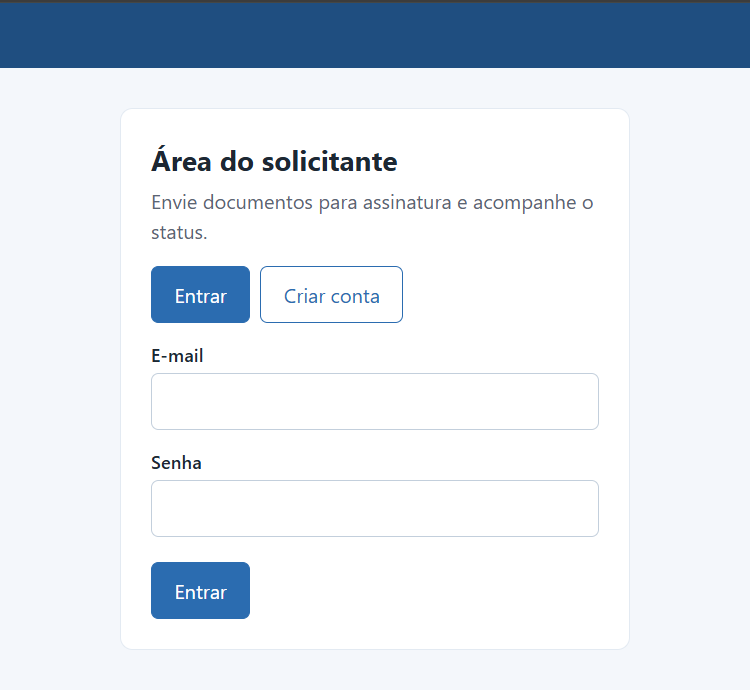
\includegraphics[width=0.5\textwidth]{tela01_entrada_solicitante.png}
    \legend{Fonte: elaborado pelo autor.}
\end{figure}
\FloatBarrier

Após a entrada, o remetente envia o documento, como mostra a Figura~\ref{fig:tela-envio}: seleciona o PDF, que é exibido na própria página, posiciona sobre ele a caixa de assinatura, arrastando-a e redimensionando-a até o local desejado, e informa o nome, o e-mail, o CPF e a data de nascimento do signatário, além da validade do link. No exemplo, a caixa foi posicionada ao lado do campo destinado à assinatura do responsável pela demanda.

\begin{figure}[htb]
    \centering
    \caption{Envio do documento com o posicionamento da caixa de assinatura}
    \label{fig:tela-envio}
    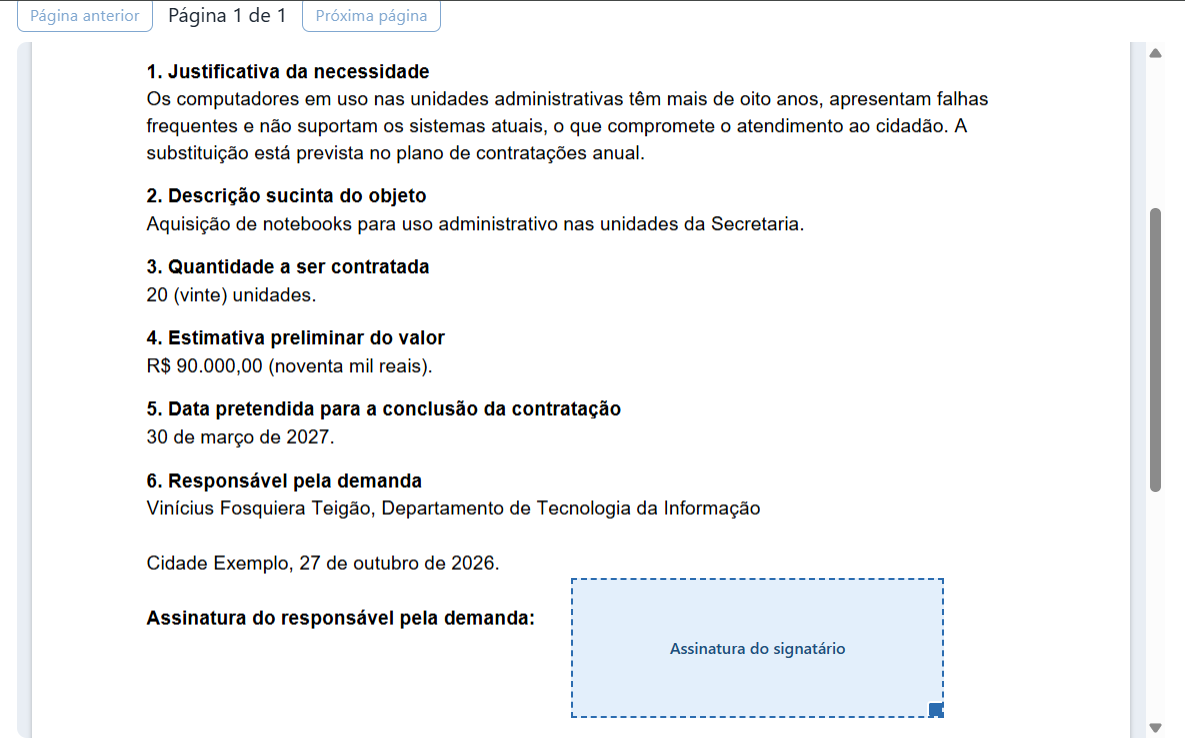
\includegraphics[width=0.85\textwidth]{tela02_envio_caixa_assinatura.png}
    \legend{Fonte: elaborado pelo autor.}
\end{figure}
\FloatBarrier

Os documentos enviados são acompanhados no painel da Figura~\ref{fig:tela-painel}, que mostra, para cada documento, o hash SHA-256, o signatário, as datas de envio e de validade, a situação do link, a situação do registro na blockchain e as ações disponíveis. No exemplo, o documento da primeira linha aguarda a assinatura e oferece a prévia da caixa, a cópia do link e a correção dos dados, enquanto o da segunda linha já foi assinado, com o registro confirmado e o link para a transação no explorador de blocos.

\begin{figure}[htb]
    \centering
    \caption{Painel de documentos do remetente}
    \label{fig:tela-painel}
    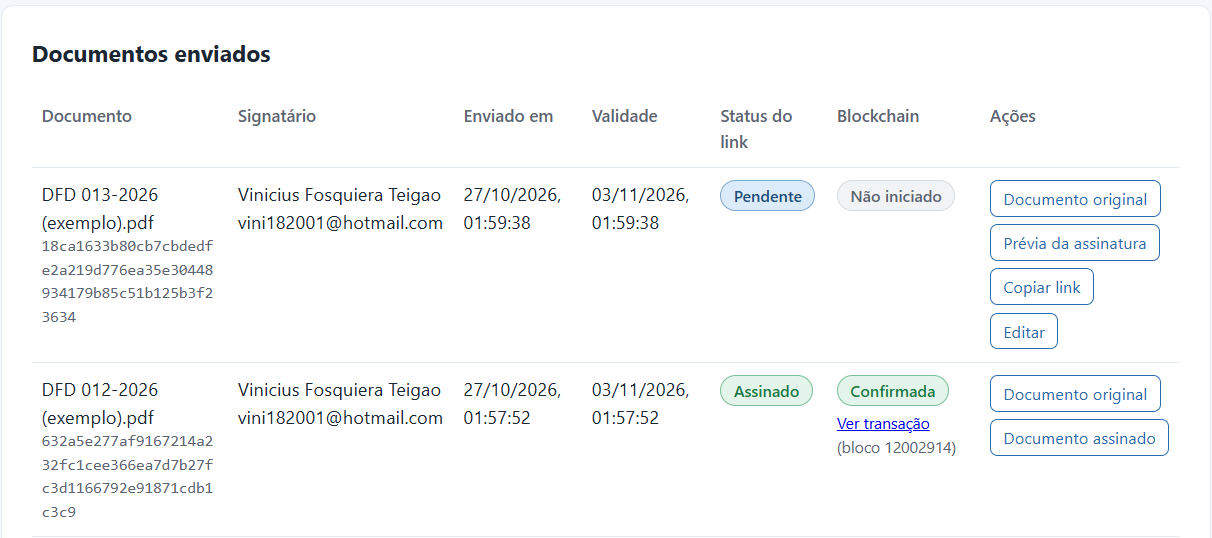
\includegraphics[width=\textwidth]{tela03_painel_documentos.png}
    \legend{Fonte: elaborado pelo autor.}
\end{figure}
\FloatBarrier

Ao abrir o link recebido, o signatário informa, na tela de verificação de identidade da Figura~\ref{fig:tela-identificacao}, o CPF e a data de nascimento e é avisado do número de tentativas restantes. Nenhuma informação do documento é exibida antes dessa verificação.

\begin{figure}[htb]
    \centering
    \caption{Verificação de identidade do signatário}
    \label{fig:tela-identificacao}
    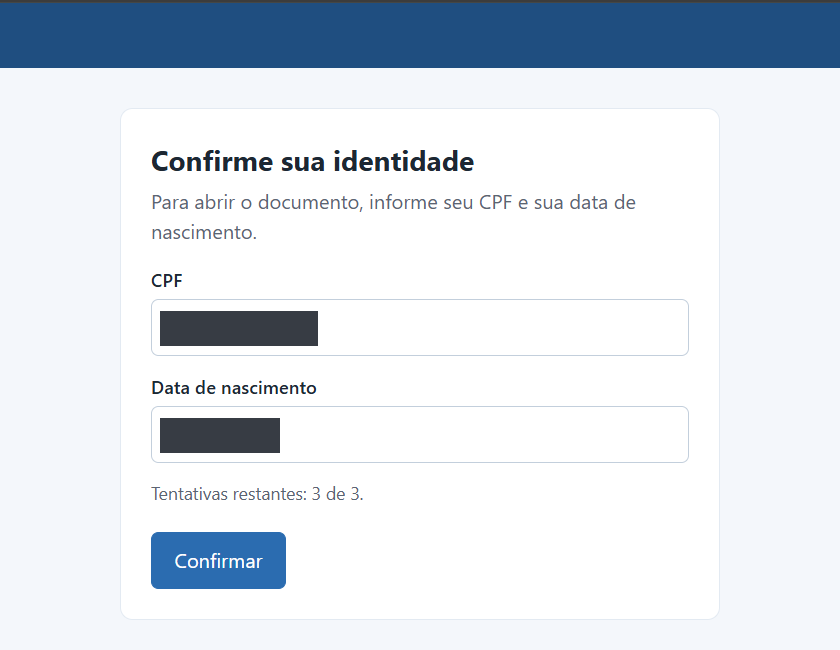
\includegraphics[width=0.55\textwidth]{tela04_identificacao_signatario.png}
    \legend{Fonte: elaborado pelo autor.}
\end{figure}
\FloatBarrier

Confirmada a identidade, o documento é exibido na própria página, como mostra a Figura~\ref{fig:tela-documento}, acompanhado da indicação de quem o enviou, do aviso sobre a página e o local em que a assinatura será inserida, da declaração de aceite e dos botões de assinatura e de recusa. O botão de assinatura só é habilitado após a marcação do aceite.

\begin{figure}[htb]
    \centering
    \caption{Visualização do documento e decisão do signatário}
    \label{fig:tela-documento}
    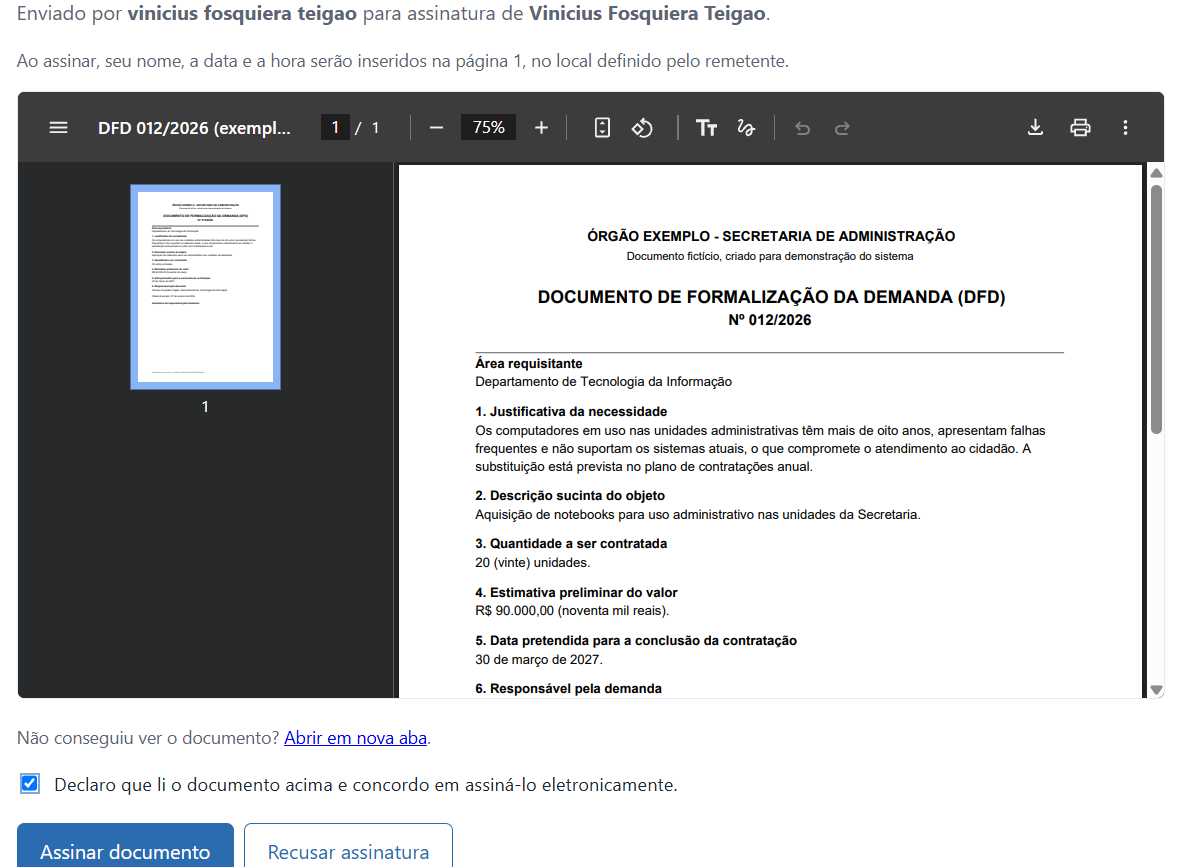
\includegraphics[width=0.85\textwidth]{tela05_documento_aceite.png}
    \legend{Fonte: elaborado pelo autor.}
\end{figure}
\FloatBarrier

Após a assinatura, a página passa a exibir o comprovante da Figura~\ref{fig:tela-comprovante}, que acompanha automaticamente o registro na blockchain e, confirmada a transação, apresenta a data e a hora da assinatura, o hash do documento, o hash das evidências, o link da transação e o número do bloco, além do acesso às versões assinada e original do documento.

\begin{figure}[htb]
    \centering
    \caption{Comprovante da assinatura com o registro confirmado}
    \label{fig:tela-comprovante}
    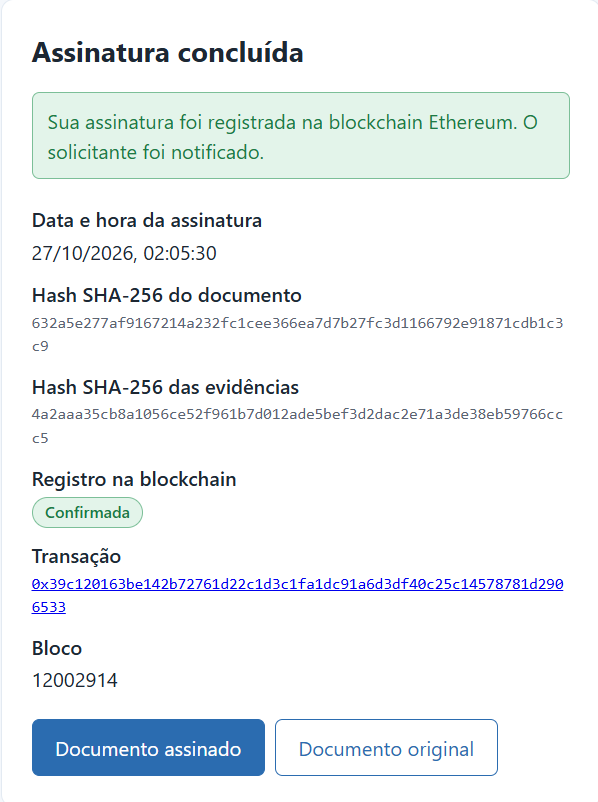
\includegraphics[width=0.45\textwidth]{tela06_comprovante.png}
    \legend{Fonte: elaborado pelo autor.}
\end{figure}
\FloatBarrier

A versão assinada, apresentada na Figura~\ref{fig:tela-assinado}, é a cópia do documento com a caixa preenchida no local definido pelo remetente, contendo o nome do signatário, a data e a hora da assinatura no horário de Brasília e o código de verificação, formado pelos 16 primeiros caracteres do hash do documento original, que permanece inalterado. O documento apresentado é fictício, criado apenas para os testes, e seu conteúdo foi gerado por uma ferramenta de inteligência artificial a partir de um \emph{prompt}.

\begin{figure}[htb]
    \centering
    \caption{Documento assinado, com a caixa de assinatura preenchida}
    \label{fig:tela-assinado}
    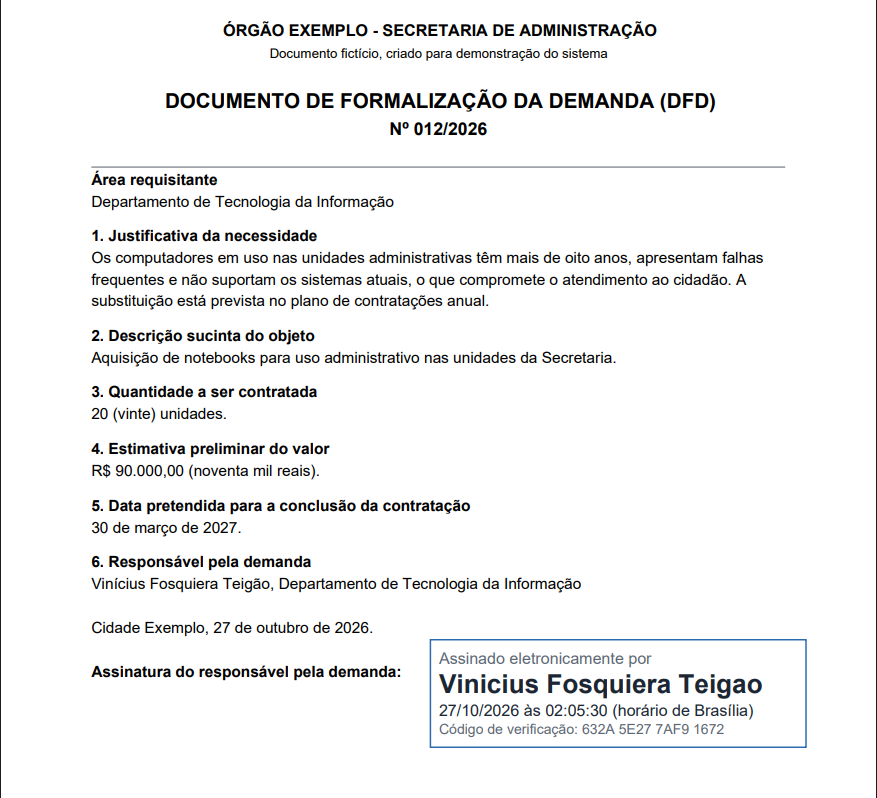
\includegraphics[width=0.7\textwidth]{tela07_documento_assinado.png}
    \legend{Fonte: elaborado pelo autor.}
\end{figure}
\FloatBarrier

A transação de registro pode ser consultada por qualquer pessoa no explorador de blocos da rede Sepolia, como mostra a Figura~\ref{fig:tela-etherscan}, que exibe a transação confirmada, o número do bloco, a carteira da plataforma como remetente e o contrato inteligente como destinatário.

\begin{figure}[htb]
    \centering
    \caption{Transação de registro no explorador de blocos da rede Sepolia}
    \label{fig:tela-etherscan}
    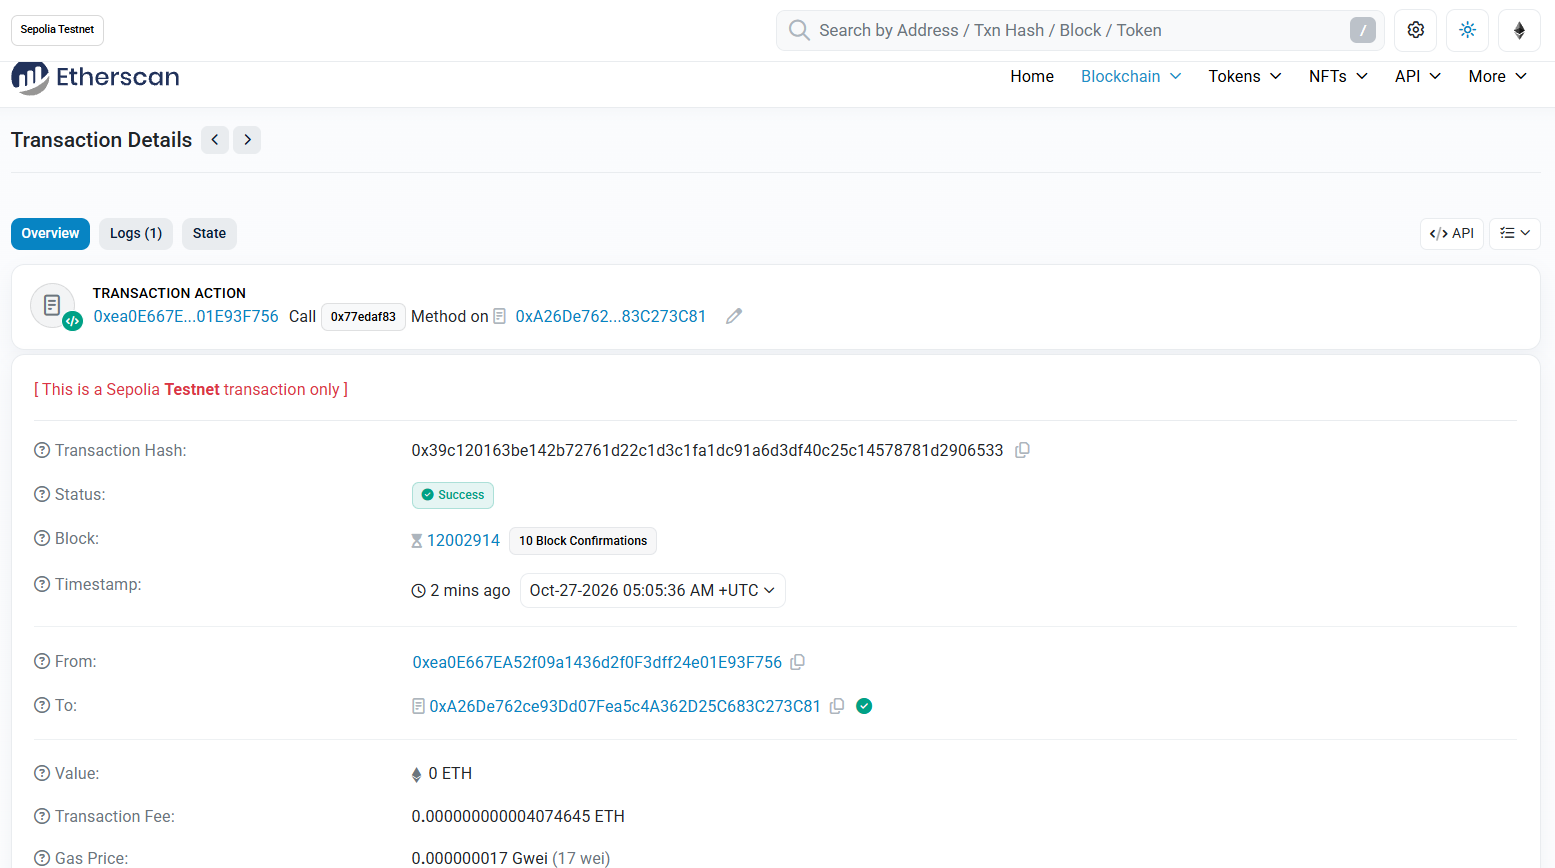
\includegraphics[width=0.8\textwidth]{tela08_transacao_etherscan.png}
    \legend{Fonte: elaborado pelo autor, com captura de tela do explorador de blocos Etherscan.}
\end{figure}
\FloatBarrier

Por fim, a Figura~\ref{fig:tela-remix} mostra o contrato implantado aberto no Remix IDE, conectado à rede Sepolia por meio da MetaMask, com o código-fonte no editor e, no painel lateral, as funções do contrato e a consulta à carteira dona, que corresponde à carteira da plataforma indicada no Quadro~\ref{quadro:implantacao}.

\begin{figure}[htb]
    \centering
    \caption{Contrato implantado aberto no Remix IDE}
    \label{fig:tela-remix}
    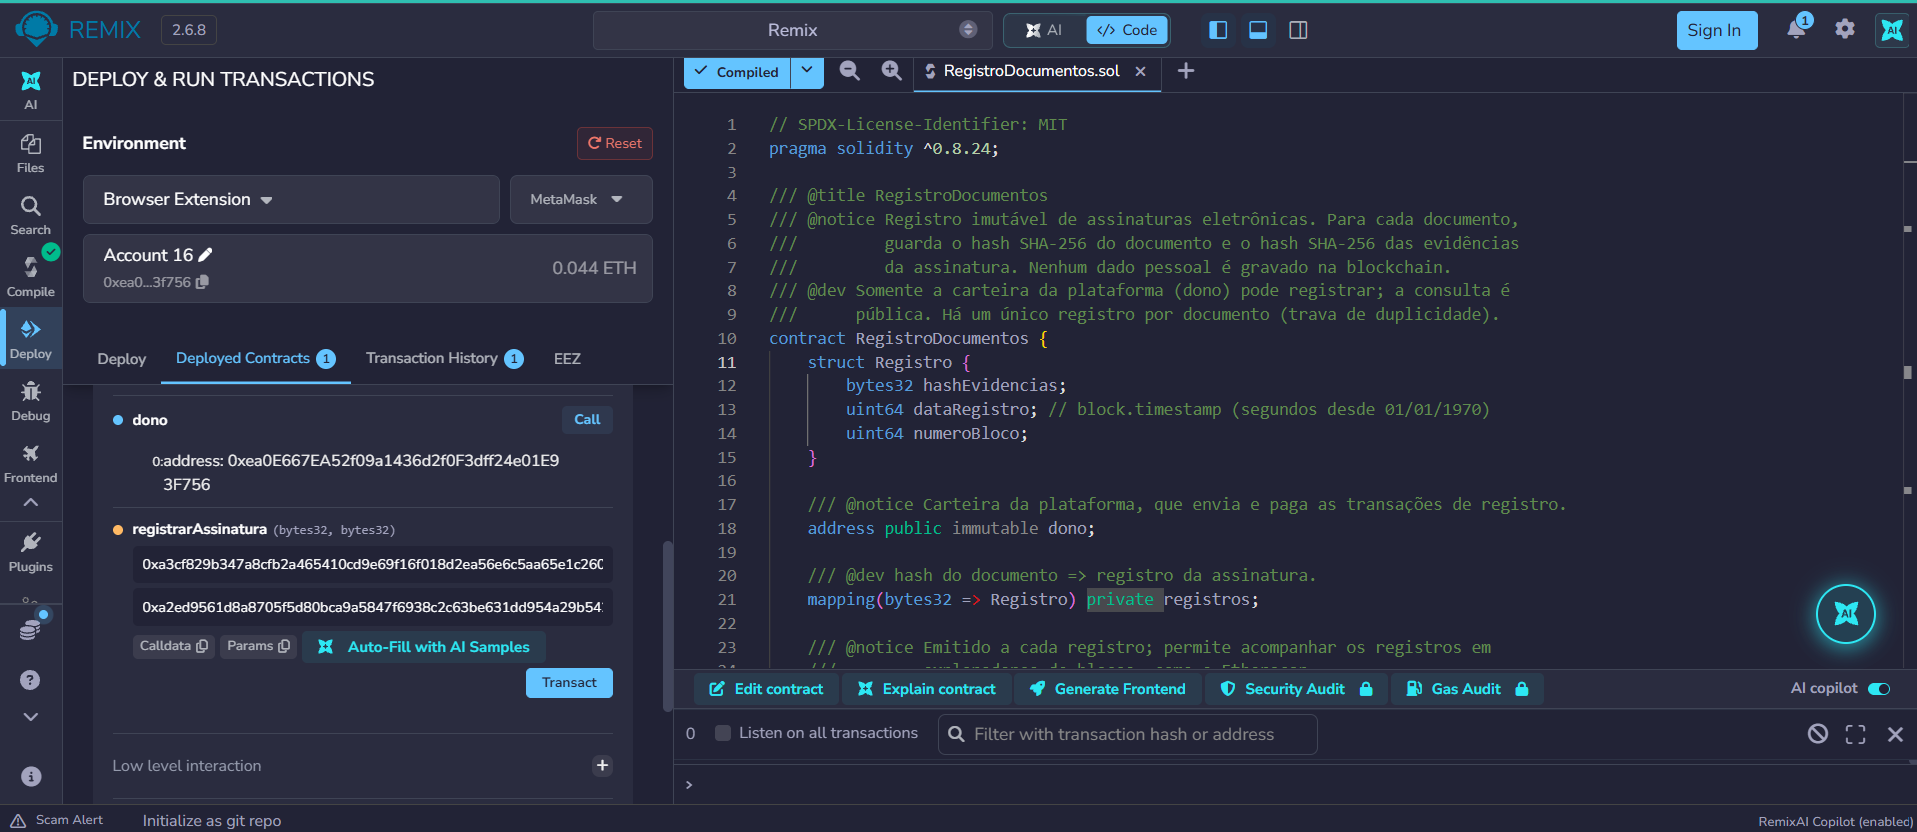
\includegraphics[width=\textwidth]{tela09_remix_contrato_implantado.png}
    \legend{Fonte: elaborado pelo autor, com captura de tela do Remix IDE.}
\end{figure}
\FloatBarrier

\section{Testes e Resultados}
\label{sec:resultados}

Esta seção relata a execução dos procedimentos de teste e validação definidos no Capítulo~\ref{sec:testes} e apresenta os resultados obtidos. A validação foi conduzida em cinco frentes: os testes automatizados das funcionalidades e da política de registro na blockchain; os testes do contrato inteligente na rede Sepolia; a coleta das métricas de desempenho e de custo, por meio da execução repetida do fluxo completo de assinatura, inclusive com signatários simultâneos; a avaliação de usabilidade por inspeção da página do signatário; e uma assinatura realizada por outra pessoa, em outro computador e em outra rede. Ao final, os resultados são confrontados com os critérios de aceitação estabelecidos naquele capítulo.

\subsection{Ambiente de Testes}
\label{sec:res-ambiente}

Os testes foram executados no ambiente descrito no Quadro~\ref{quadro:ambiente}. O \emph{backend}, o banco de dados e o programa que simulou os usuários funcionaram no mesmo computador, de modo que os tempos de resposta medidos não incluem a latência de uma rede entre o navegador do usuário e o servidor. Os registros foram feitos no contrato implantado na rede Sepolia, descrito no Capítulo~\ref{sec:impl-contrato}, por meio do mesmo provedor de acesso utilizado pelo sistema. Somente o teste descrito no Capítulo~\ref{sec:res-remoto} envolveu um navegador em outro computador.

\begin{quadro}[htb]
    \caption{Ambiente de execução dos testes}
    \label{quadro:ambiente}
    \centering
    \small
    \begin{tabular}{L{4.0cm}L{10.8cm}}
        \toprule
        \textbf{Item} & \textbf{Descrição} \\
        \midrule
        Computador & Notebook com processador AMD Ryzen 7 5700U, 16 núcleos lógicos e 15 GB de memória disponível \\
        Sistema operacional & Windows 11 Home \\
        Software & Node.js 24.20 e MySQL 8.0.46, com as demais tecnologias do Quadro~\ref{quadro:tecnologias} \\
        Rede & Sepolia, com o contrato e a carteira da plataforma do Quadro~\ref{quadro:implantacao}, acessada pelo RPC público PublicNode \\
        Banco de dados & Banco exclusivo para a coleta de métricas, criado pelo mesmo \emph{script} do Capítulo~\ref{sec:banco}, sem afetar os dados do sistema \\
        Documento de teste & PDF de duas páginas, com cerca de 2,3 KB, gerado com conteúdo distinto para cada amostra, uma vez que o contrato admite um único registro por documento \\
        Período da coleta & De 26/10/2026, às 23h55, a 27/10/2026, às 0h10 \\
        \bottomrule
    \end{tabular}
    \legend{Fonte: elaborado pelo autor.}
\end{quadro}

\subsection{Testes Funcionais Automatizados}
\label{sec:res-funcionais}

Os testes funcionais e de integração foram automatizados com o executor de testes do Node.js e somam 37 casos, todos aprovados na execução final, cuja saída está no Apêndice~\ref{ap:testes}. Vinte deles percorrem o fluxo pela API do \emph{backend}, em um banco de dados separado, e verificam o envio, a identificação, a visualização, a assinatura, a recusa, a expiração, a correção de dados e o controle de acesso; seis verificam a geração da cópia com a caixa de assinatura, inclusive em páginas giradas e com área visível deslocada; e onze verificam a política de registro descrita no Capítulo~\ref{sec:impl-contrato}. Nestes últimos, a rede Ethereum é substituída por uma simulação, porque falhas como a não inclusão de uma transação no prazo, a indisponibilidade do provedor de acesso e a falta de saldo não podem ser provocadas sob demanda na rede real. A correspondência entre os cenários previstos no Capítulo~\ref{sec:cenarios-teste} e as verificações realizadas é apresentada no Quadro~\ref{quadro:cenarios}.

\begin{quadro}[htb]
    \caption{Cenários de teste e verificações realizadas}
    \label{quadro:cenarios}
    \centering
    \small
    \begin{tabular}{L{4.0cm}L{10.8cm}}
        \toprule
        \textbf{Cenário} & \textbf{Verificações} \\
        \midrule
        Fluxo principal & Fluxo completo com conferência do hash, coleta das evidências e uso único do link; confirmação do registro na primeira tentativa, com gravação da transação, do bloco, do gas e do custo; 60 registros na rede Sepolia, descritos no Capítulo~\ref{sec:res-blockchain} \\
        Link expirado ou já utilizado & Prazo vencido leva ao estado \elem{Expirado}; link já assinado é recusado; documento em estado final não pode ser editado nem ter o link reexibido; token inexistente ou malformado é rejeitado \\
        CPF ou data de nascimento incorretos & Três tentativas erradas bloqueiam o link e notificam o remetente; a correção do CPF pelo remetente zera as tentativas e exige nova identificação \\
        Caixa de assinatura & Conversão da posição para o PDF em todas as rotações de página; caixa obrigatória e dentro de uma página existente; prévia antes da assinatura; cópia preenchida, com hash incluído nas evidências e original inalterado \\
        Recusa da assinatura & Recusa explícita leva ao estado \elem{Recusado} \\
        Falha na transação & Reenvio com o mesmo \emph{nonce} e taxa ajustada; estado \elem{Falha} após três tentativas; indisponibilidade do provedor tratada como falha transitória; reversão e saldo insuficiente tratados como falhas determinísticas, sem reenvio; consulta prévia que evita registro duplicado; retomada após reinício do servidor \\
        Acesso simultâneo & Execução do fluxo com 5, 10 e 25 signatários simultâneos, descrita no Capítulo~\ref{sec:res-desempenho} \\
        Integridade e acesso & Documento alterado após o envio bloqueia a assinatura; PDF idêntico a outro em processo é recusado; remetente não acessa documentos de outro remetente \\
        \bottomrule
    \end{tabular}
    \legend{Fonte: elaborado pelo autor.}
\end{quadro}

\subsection{Testes do Contrato Inteligente}
\label{sec:res-contrato}

Os testes do contrato inteligente foram realizados no Remix IDE. O registro e a consulta foram testados na Remix VM antes da implantação e confirmados, depois dela, na rede Sepolia, em que todos os registros enviados pelo sistema foram aceitos. Os testes de exceção foram executados diretamente sobre o contrato implantado na Sepolia, com o Remix conectado à MetaMask, utilizando a carteira da plataforma e uma segunda conta, criada apenas para esse fim. Os procedimentos e os resultados obtidos são apresentados no Quadro~\ref{quadro:testes-contrato}.

\begin{quadro}[htb]
    \caption{Testes do contrato inteligente}
    \label{quadro:testes-contrato}
    \centering
    \small
    \begin{tabular}{L{2.5cm}L{5.3cm}L{6.7cm}}
        \toprule
        \textbf{Teste} & \textbf{Procedimento} & \textbf{Resultado obtido} \\
        \midrule
        Registro & A carteira da plataforma registra o hash de um documento e o hash das evidências & Registro aceito e evento emitido, na Remix VM e em todos os registros feitos pelo sistema na Sepolia \\
        Consulta & Consulta do registro de um documento assinado em 25/10/2026 & Documento registrado, com o hash das evidências gravado pelo sistema, a data e a hora 25/10/2026 18:40:48 e o bloco 11.993.591 \\
        Duplicidade & A carteira da plataforma tenta registrar novamente o mesmo documento & Transação revertida com o erro \texttt{DocumentoJaRegistrado}, no bloco 12.002.091; a consulta posterior manteve os dados originais \\
        Outra conta & Uma conta que não é a dona do contrato tenta registrar um documento novo & Transação revertida com o erro \texttt{SomenteDono}, no bloco 12.002.197; a consulta feita por essa conta funcionou normalmente \\
        Hash não registrado & Consulta do documento usado no teste anterior & Documento não registrado, com valores nulos, o que confirma que a tentativa recusada não gravou dados \\
        \bottomrule
    \end{tabular}
    \legend{Fonte: elaborado pelo autor.}
\end{quadro}

Nos dois testes de exceção, o Remix alertou, antes do envio, que a execução seria revertida e exibiu o erro pelo seu identificador de quatro bytes: \texttt{0x142be92f} no teste de duplicidade e \texttt{0x007581da} no teste de outra conta, que correspondem, respectivamente, aos erros \texttt{DocumentoJaRegistrado} e \texttt{SomenteDono} definidos no contrato. As transações foram enviadas mesmo assim, para que a recusa ficasse registrada na rede pública: ambas foram incluídas em bloco com status de falha, sem emissão de evento, e consumiram 19.352 unidades de gas cada uma. Os resultados demonstram que um registro não pode ser sobrescrito, que apenas a carteira da plataforma pode registrar e que a consulta é aberta a qualquer conta, sem custo, o que sustenta a verificação por terceiros prevista no requisito RF5.

Além do controle de acesso e da unicidade do registro, verificados nesses testes, o contrato foi confrontado com os problemas de segurança levantados por \citeonline{alharby2017} e discutidos no Capítulo~\ref{sec:desafios}. Cinco deles dizem respeito a falhas de código: a dependência da ordem das transações, a dependência do horário do bloco, o tratamento inadequado de exceções, a reentrância e o uso de dados externos não confiáveis; o sexto, as atividades criminosas, refere-se ao emprego de contratos para fins ilícitos. A superfície de ataque do contrato, cujo código-fonte está no Apêndice~\ref{ap:contrato}, é reduzida. Há uma única função de escrita, restrita à carteira da plataforma, de modo que nenhuma outra conta pode registrar e o resultado de um registro não depende da ordem em que as transações são incluídas no bloco. O horário do bloco é gravado no registro e só é comparado com zero, para indicar se o documento já foi registrado, de modo que nenhuma decisão do contrato depende do seu valor exato. O contrato não chama outros contratos, o que afasta o tratamento inadequado de exceções e a reentrância, e não consulta dados externos à blockchain. Nenhuma de suas funções aceita pagamento em ether, o contrato não mantém saldos nem realiza operações aritméticas sobre valores, e a versão 0.8 da linguagem Solidity interrompe a execução em caso de estouro aritmético. Também não há laços, cujo custo poderia crescer com o número de registros, nem mecanismos de atualização ou de destruição do código. O risco remanescente concentra-se fora do contrato, na chave privada da carteira da plataforma, mantida no servidor: quem a obtivesse poderia registrar hashes indevidos, inclusive ocupar antecipadamente o registro de um documento legítimo, embora não pudesse alterar registros existentes; e, como a dona do contrato é definida na implantação e não pode ser trocada, a substituição da chave exigiria a implantação de um novo contrato.

O código-fonte do contrato foi submetido, ainda, à análise estática da ferramenta gratuita Slither \cite{feist2019}, na versão 0.11.6, com o mesmo compilador da implantação, Solidity 0.8.34. Dos 102 detectores executados, nenhum apontou problema de severidade alta ou média, nem observação informativa ou de otimização. Foram relatados apenas dois resultados de severidade baixa, ambos do detector de uso do horário do bloco em comparações, nas funções de registro e de consulta. Nos dois casos, o campo comparado é a data do registro, que guarda o horário do bloco e é comparada com zero para indicar se o documento já foi registrado, como descrito acima. Como todo bloco possui horário diferente de zero, o resultado da comparação não depende do valor exato do horário, e os dois apontamentos não representam risco ao contrato. A saída completa da análise está no Apêndice~\ref{ap:slither}.

\subsection{Desempenho do Backend}
\label{sec:res-desempenho}

Para medir o desempenho e o registro na blockchain em condições próximas às de uso, foi desenvolvido um \emph{script} que inicia uma instância do sistema com banco de dados próprio e percorre, pela API, o mesmo fluxo realizado pelas páginas: o remetente envia o PDF com a caixa de assinatura posicionada; o signatário abre o link, informa CPF e data de nascimento, abre o documento, cujo hash é conferido com o do arquivo enviado, e assina; e, por fim, o remetente consulta o painel. O tempo de resposta de cada etapa foi medido entre o envio da requisição e o recebimento completo da resposta. Foram executados quatro cenários: vinte assinaturas, uma por vez, cada uma aguardando a confirmação do próprio registro antes da seguinte, e lotes de 5, 10 e 25 signatários iniciando o fluxo ao mesmo tempo, o que corresponde ao cenário de acesso simultâneo previsto no Capítulo~\ref{sec:cenarios-teste}. No total, foram executados 60 fluxos, com 360 requisições, todos concluídos sem erro.

Os tempos médios de cada etapa e os respectivos percentis 95 (P95), valor abaixo do qual estão 95\% das medições, são apresentados no Quadro~\ref{quadro:desempenho}. Com um signatário por vez, todas as etapas responderam, em média, em menos de 50 ms. O envio do documento é a etapa mais demorada, por envolver o recebimento e a leitura do PDF, o cálculo do hash e a gravação no banco de dados, seguido da assinatura, que inclui a nova conferência do hash, a geração da cópia com a caixa preenchida e o cálculo do hash das evidências. Com o aumento da simultaneidade, os tempos cresceram de forma gradual e sem erros: com 25 signatários ao mesmo tempo, a maior resposta observada foi de 302 ms, na assinatura, e os 25 fluxos, com 150 requisições, foram concluídos em 0,8 s.

\begin{quadro}[htb]
    \caption{Tempo de resposta do \emph{backend}, em milissegundos: média e, entre parênteses, P95}
    \label{quadro:desempenho}
    \centering
    \small
    \begin{tabular}{L{3.4cm}*{4}{>{\raggedleft\arraybackslash}p{2.4cm}}}
        \toprule
        \textbf{Etapa} & \textbf{Um por vez} & \textbf{5 simultâneos} & \textbf{10 simultâneos} & \textbf{25 simultâneos} \\
        \midrule
        Envio do documento & 49,8 (69,9) & 104,9 (106,3) & 150,8 (197,8) & 210,1 (226,8) \\
        Abertura do link & 11,3 (15,9) & 19,1 (23,1) & 27,7 (46,7) & 65,8 (97,2) \\
        Identificação & 19,0 (24,6) & 17,6 (19,0) & 45,0 (60,9) & 71,3 (86,0) \\
        Abertura do PDF & 17,1 (22,6) & 18,3 (19,2) & 45,2 (70,0) & 73,9 (100,9) \\
        Assinatura & 32,9 (41,0) & 60,3 (65,8) & 104,3 (140,4) & 172,7 (298,6) \\
        Painel do remetente & 14,7 (21,2) & 12,6 (15,3) & 31,9 (55,3) & 101,4 (154,7) \\
        \midrule
        Amostras por etapa & 20 & 5 & 10 & 25 \\
        \bottomrule
    \end{tabular}
    \legend{Fonte: elaborado pelo autor.\newline Nota: o \emph{backend}, o banco de dados e o programa que simulou os usuários funcionaram no mesmo computador; os tempos não incluem a latência de rede entre o navegador do usuário e o servidor.}
\end{quadro}

\subsection{Registro na Blockchain}
\label{sec:res-blockchain}

Os 60 registros produzidos pela coleta foram confirmados na rede Sepolia, todos na primeira tentativa de envio, o que corresponde a uma taxa de erro de 0\% nas transações. Como nenhuma falha transitória ocorreu durante a coleta, o reenvio previsto na política de registro não chegou a ser acionado na rede real, e o seu funcionamento permanece demonstrado pelos testes com rede simulada descritos no Capítulo~\ref{sec:res-funcionais} e listados no Apêndice~\ref{ap:testes}.

O tempo de confirmação, medido entre o envio da transação e a obtenção do seu recibo pelo \emph{backend}, teve média de 13,1 s, mediana de 10,0 s, P95 de 23,4 s e valores entre 4,8 s e 46,2 s. Desse tempo, em média 10,7 s correspondem à inclusão em bloco, calculada a partir do horário registrado no próprio bloco, e o restante decorre do intervalo de 2 segundos com que o \emph{backend} consulta o recibo da transação. O resultado é coerente com o ritmo de produção de blocos observado na Sepolia durante os testes do contrato, de 106 blocos em 21 minutos e 48 segundos, ou um bloco a cada 12,3 s em média: a maior parte das transações foi incluída no bloco seguinte ao envio, e as mais demoradas, em um dos blocos subsequentes.

Como o registro é feito por uma fila, um por vez, a partir da mesma carteira, o intervalo entre a assinatura e o envio da transação depende da quantidade de registros à frente. Com um signatário por vez, esse intervalo, que inclui a consulta prévia ao contrato, foi de 1,2 s em média; com signatários simultâneos, cresceu com o tamanho do lote, como mostra o Quadro~\ref{quadro:fila}. No lote de 25 signatários, o último registro foi confirmado 6,4 minutos após o início do cenário, o que corresponde a cerca de 15 s por registro, ou aproximadamente quatro registros por minuto. No lote de 5, uma das transações levou 45,5 s para ser confirmada, o que elevou a média por registro desse cenário.

\begin{quadro}[htb]
    \caption{Registro na blockchain por cenário}
    \label{quadro:fila}
    \centering
    \small
    \begin{tabular}{L{2.4cm}L{1.9cm}L{2.5cm}L{2.4cm}L{1.9cm}L{1.9cm}}
        \toprule
        \textbf{Cenário} & \textbf{Registros} & \textbf{Confirmação (mediana)} & \textbf{Maior espera até o envio} & \textbf{Duração total} & \textbf{Média por registro} \\
        \midrule
        Um por vez & 20 & 9,7 s & 1,7 s & 258,7 s & 12,9 s \\
        5 simultâneos & 5 & 12,1 s & 96,9 s & 109,3 s & 21,9 s \\
        10 simultâneos & 10 & 10,8 s & 120,0 s & 130,9 s & 13,1 s \\
        25 simultâneos & 25 & 10,2 s & 360,0 s & 383,8 s & 15,4 s \\
        \bottomrule
    \end{tabular}
    \legend{Fonte: elaborado pelo autor.}
\end{quadro}

A assinatura propriamente dita, com as evidências gravadas no banco de dados, é concluída em fração de segundo, conforme o Capítulo~\ref{sec:res-desempenho}; o que se estende é a espera pelo comprovante com a transação confirmada, que, com um signatário por vez, teve mediana de 11,2 s e P95 de 21,9 s contados a partir da assinatura. Com signatários simultâneos, em razão da fila, o P95 desse intervalo foi de 108,7 s, 129,7 s e 358,3 s nos lotes de 5, 10 e 25 signatários, respectivamente. A página do signatário acompanha a situação do registro a cada 3 segundos, por até 6 minutos; esgotado esse prazo, informa que a assinatura foi gravada e que o registro continua em andamento, com a conclusão acompanhada pelo remetente no painel. No lote de 25 signatários, essa situação ocorreria com um deles, cujo registro foi confirmado 6,4 minutos após a assinatura.

\subsection{Custo das Transações}
\label{sec:res-custo}

Cada registro consumiu entre 239.661 e 239.685 unidades de gas na rede Sepolia, e a implantação do contrato, 2.488.245 unidades, conforme o Quadro~\ref{quadro:implantacao}. Nessa rede, o custo em ether não tem significado econômico: o ether de teste é obtido gratuitamente, e o preço do gas durante a coleta foi tão baixo que cada registro custou cerca de $5 \times 10^{-12}$ ETH. A avaliação da viabilidade financeira exige, portanto, estimar o custo das mesmas operações na rede principal da Ethereum.

Os valores medidos na Sepolia são bem superiores aos esperados para o código do contrato porque essa rede recebeu, em 6 de outubro de 2026, a atualização Glamsterdam, que ainda não tem data definida para a rede principal \cite{beiko2024}. Entre as alterações dessa atualização está a EIP-8037, que eleva o custo de criação de novos dados no estado da blockchain \cite{silva2025}: a gravação de um valor em uma posição de armazenamento vazia passou de 20.000 para 97.920 unidades de gas, o custo fixo de criação de um contrato, que a norma iguala ao de criação de uma nova conta, de 32.000 para 183.600, e cada byte de código publicado, de 200 para 1.530 unidades. Como cada registro grava duas posições de armazenamento novas, a regra explica 155.840 das 169.092 unidades de diferença entre o valor medido e o estimado para a rede principal, cerca de 92\%, e o restante decorre de outras alterações de custo da mesma atualização. Na implantação, a diferença prevista pela regra para um código de 1.475 bytes, de 2.113.350 unidades, coincide praticamente com a diferença medida, de 2.112.515 unidades.

Para a rede principal, o consumo de gas foi estimado por simulação, sem envio de transação: um nó dessa rede calculou o gas da implantação a partir do mesmo código compilado e o gas de um registro com o código do contrato inserido, apenas na simulação, no endereço do contrato. Os resultados, 375.730 unidades para a implantação e 70.593 para cada registro, refletem as regras atualmente em vigor nessa rede. O preço do gas foi obtido da própria rede principal, a partir do histórico de taxas de 1.024 blocos consecutivos em 22 dias distintos dos 30 dias anteriores a 27 de outubro de 2026, num total de 22.528 blocos: o preço efetivo, soma da taxa base com a taxa de prioridade mediana de cada bloco, teve mediana de 0,0975 \emph{gwei} e percentil 90 (P90) de 0,384 \emph{gwei}. A conversão para reais utilizou a cotação de R\$~12.402,53 por ether em 27 de outubro de 2026 \cite{coingecko2026}. As estimativas resultantes estão no Quadro~\ref{quadro:custos}.

\begin{quadro}[htb]
    \caption{Estimativa de custo na rede principal da Ethereum}
    \label{quadro:custos}
    \centering
    \small
    \begin{tabular}{L{3.6cm}L{2.6cm}rrr}
        \toprule
        \textbf{Operação} & \textbf{Regras de cobrança} & \textbf{Gas} & \textbf{Preço mediano} & \textbf{Preço P90} \\
        \midrule
        Registro de uma assinatura & Atuais & 70.593 & R\$~0,09 & R\$~0,34 \\
         & Glamsterdam & 239.685 & R\$~0,29 & R\$~1,14 \\
        \midrule
        Implantação do contrato & Atuais & 375.730 & R\$~0,45 & R\$~1,79 \\
         & Glamsterdam & 2.488.245 & R\$~3,01 & R\$~11,86 \\
        \bottomrule
    \end{tabular}
    \legend{Fonte: elaborado pelo autor.}
\end{quadro}

Pelas regras atuais da rede principal, o registro de uma assinatura custaria cerca de R\$~0,09 com o preço mediano do gas e R\$~0,34 com o P90, e a implantação do contrato, realizada uma única vez, cerca de R\$~0,45 e R\$~1,79. Caso a atualização Glamsterdam seja adotada na rede principal com os mesmos parâmetros em vigor na Sepolia, o registro passaria a custar cerca de R\$~0,29 e R\$~1,14, e a implantação, R\$~3,01 e R\$~11,86, mantidos os preços do gas e do ether. Em qualquer dos casos, o custo por assinatura fica entre alguns centavos e pouco mais de um real, pago pela plataforma, sem custo algum para o signatário. Esses valores devem ser lidos como ordem de grandeza: a cotação do ether variou entre R\$~11.570 e R\$~14.246 nos 30 dias anteriores \cite{coingecko2026}, o preço do gas oscila com a demanda da rede, e a EIP-8037 ainda pode ter seus parâmetros alterados antes da adoção na rede principal \cite{silva2025}.

\subsection{Defeito Encontrado no Teste de Carga}
\label{sec:res-defeito}

A primeira execução do \emph{script}, feita para validá-lo com apenas dois signatários simultâneos, revelou um defeito: a consulta ao painel do remetente retornou erro interno enquanto o outro signatário assinava. O registro do servidor indicou um impasse (\emph{deadlock}) no banco de dados. A rotina que marca como expirados os links vencidos, executada, entre outros momentos, a cada consulta ao painel e a cada acesso ao link, atualizava a tabela de links com uma condição sobre o status, o que levava o banco de dados a travar, no índice de status, todos os links ainda em aberto. Ao mesmo tempo, a assinatura do outro signatário alterava o status do seu próprio link, de modo que cada operação passou a aguardar uma trava mantida pela outra, e o gerenciador de banco de dados desfez uma delas. Nessa execução, a operação desfeita foi a consulta ao painel, mas poderia ter sido a própria assinatura.

A rotina foi corrigida para localizar os links vencidos por meio de uma leitura sem travas e atualizar apenas esses links, identificados pela chave primária. Assim, no caso comum, em que nenhum link venceu, nenhuma trava é obtida, e, quando há links vencidos, somente eles são travados. Após a correção, os 37 testes automatizados continuaram aprovados, e a coleta completa, com até 25 signatários simultâneos, não registrou nenhum erro. O episódio mostra a importância do cenário de acesso simultâneo previsto no Capítulo~\ref{sec:cenarios-teste}: o defeito não se manifestava nos testes com um usuário por vez.

\subsection{Avaliação de Usabilidade por Inspeção}
\label{sec:res-usabilidade}

A inspeção da página do signatário, realizada pelo autor, identificou três telas, apresentadas em sequência na mesma página do navegador e mostradas nas Figuras~\ref{fig:tela-identificacao}, \ref{fig:tela-documento} e~\ref{fig:tela-comprovante}. Na primeira, o signatário informa o CPF e a data de nascimento e confirma. Na segunda, o documento é exibido na própria página, acompanhado da declaração de aceite e dos botões de assinatura e de recusa. Na terceira, é apresentado o comprovante, que acompanha automaticamente o registro na blockchain e exibe o link da transação após a confirmação. Para assinar, além do preenchimento dos dois campos, o signatário executa três ações: confirmar a identidade, marcar a declaração de aceite e acionar o botão de assinatura.

Em nenhuma etapa são exigidos carteira digital, criptomoeda, pagamento de taxa, instalação de software ou conhecimento sobre blockchain: o signatário utiliza apenas o navegador, e a transação é enviada e paga pela carteira da plataforma. Esse resultado contrasta com o procedimento necessário para interagir diretamente com o contrato, empregado nos testes descritos no Capítulo~\ref{sec:res-contrato}, que exigiu a instalação da extensão MetaMask, a importação de uma carteira, a obtenção de saldo na rede de testes e a confirmação de cada transação, inclusive com o ajuste manual do limite de gas para que uma delas pudesse ser enviada.

\subsection{Teste de Acesso Remoto}
\label{sec:res-remoto}

Nos testes descritos até aqui, o navegador e o servidor funcionaram no mesmo computador. Para verificar o uso do link a partir de outro local, o servidor foi exposto à internet por um túnel temporário do serviço Cloudflare Tunnel, que gera um endereço público e encaminha as requisições recebidas ao computador do servidor. O link de um documento foi então enviado a outra pessoa, que o abriu em outro computador, conectado a outra rede, e concluiu a assinatura em 27/10/2026. O registro foi confirmado na rede Sepolia na primeira tentativa, no bloco 12.006.803, 7,3 s após o envio da transação.

Como as requisições recebidas pelo túnel chegam ao servidor a partir do próprio computador, o \emph{backend} foi ajustado para obter o endereço IP do signatário de um cabeçalho acrescentado pelo túnel, aceito somente quando a conexão provém do próprio computador. Sem esse ajuste, o acesso, a identificação, a visualização e a assinatura seriam atribuídos ao endereço local do servidor, e o endereço IP perderia o valor como evidência. Na execução realizada, a trilha de auditoria e as evidências da assinatura registraram o endereço IP público do signatário, pertencente a outra rede. Por se tratar de uma única execução, o teste demonstra o funcionamento do fluxo entre redes diferentes, sem medir desempenho nem usabilidade.

\subsection{Atendimento aos Critérios de Aceitação}

Confrontados com os critérios de aceitação definidos no Capítulo~\ref{sec:testes}, os resultados obtidos permitem as seguintes constatações:
\begin{itemize}
\item As funcionalidades correspondentes aos requisitos RF1 a RF7 operaram corretamente nos cenários de teste, conforme os 37 testes automatizados, cuja saída está no Apêndice~\ref{ap:testes}, e os 60 fluxos completos executados sem erro, nos quais o hash do documento apresentado ao signatário coincidiu sempre com o do arquivo enviado;
\item O registro mostrou-se imutável e verificável por terceiros, em atendimento ao requisito RF5: o contrato recusou a gravação repetida de um documento e o registro por outra conta, e a consulta foi realizada sem custo por uma conta diferente da carteira da plataforma;
\item A integridade exigida pelo requisito RNF1 foi preservada: além da coincidência dos hashes nos 60 fluxos, o documento alterado após o envio teve a assinatura bloqueada nos testes automatizados, e cada assinatura teve o hash das evidências registrado no contrato junto com o hash do documento, sem o envio de dados pessoais à rede. A atribuição de autoria, por sua vez, continua dependente das evidências coletadas pela plataforma;
\item Os limites do requisito RNF3 foram atendidos em parte. As operações do \emph{backend} responderam em menos de 1 s no P95 em todos os cenários, com o maior P95, de 298,6 ms, na assinatura com 25 signatários simultâneos. O comprovante com a transação confirmada foi emitido em até 60 s no cenário de um signatário por vez, com P95 de 21,9 s, mas não com signatários simultâneos, em que o P95 chegou a 108,7 s, 129,7 s e 358,3 s nos lotes de 5, 10 e 25 signatários, porque a fila de registro limita a vazão a cerca de quatro registros por minuto;
\item O signatário conclui o fluxo exclusivamente pelo navegador, sem carteira digital, criptomoeda ou instalação de software, em atendimento ao requisito RNF2;
\item O link resistiu aos riscos previstos no requisito RNF5: o link já utilizado e o link vencido foram recusados, o token inexistente ou malformado foi rejeitado, a identificação foi bloqueada após três tentativas erradas e o documento permaneceu inacessível antes da confirmação da identidade;
\item A conformidade legal prevista no requisito RNF4 foi avaliada de forma analítica, e não por teste. Pela classificação da Lei n\textsuperscript{o} 14.063/2020, a assinatura produzida pelo sistema permite identificar o signatário e associa os seus dados ao documento, características da assinatura eletrônica simples; não utiliza o certificado ICP-Brasil exigido na qualificada, e a identificação por CPF e data de nascimento não se baseia em dados sob controle exclusivo do signatário, como requer a avançada \cite{brasil2020}. O conjunto de evidências pode ser apresentado como meio de prova com fundamento na liberdade probatória do art. 369 do Código de Processo Civil \cite{brasil2015}, mas o seu peso probatório não foi avaliado por especialistas.
\end{itemize}

Esses resultados devem ser considerados à luz das condições em que foram obtidos: os registros foram feitos em uma rede de testes; o servidor e o programa que simulou os usuários funcionaram no mesmo computador, e o acesso a partir de outra rede foi verificado em uma única assinatura, por meio de um túnel temporário; os documentos de teste eram pequenos, de cerca de 2,3 KB, enquanto documentos reais podem ter centenas de quilobytes, o que tende a aumentar os tempos de envio e de assinatura; nenhuma falha de rede ocorreu durante a coleta, de modo que o reenvio foi verificado apenas com rede simulada; e a usabilidade foi avaliada por inspeção, sem a participação de usuários.

% =================================================================
\chapter{Conclusões}
% =================================================================

Este trabalho partiu da pergunta de como desenvolver um sistema de assinatura eletrônica via link, com registro imutável em blockchain por meio de contratos inteligentes, que fosse tecnicamente viável, seguro e acessível a todos os tipos de usuários. Os resultados obtidos indicam que essa combinação é viável quando a complexidade da blockchain fica inteiramente a cargo da plataforma: o signatário interage apenas com uma página \emph{web}, a carteira da plataforma assina e paga as transações, e a blockchain recebe somente o hash do documento e o hash das evidências da assinatura, de modo que os dados pessoais permanecem fora da cadeia. O protótipo desenvolvido realiza esse percurso de ponta a ponta, do envio do documento pelo remetente até o registro confirmado na rede Sepolia e a sua consulta pública.

O primeiro objetivo específico, projetar e implementar o contrato inteligente, foi atingido com o contrato RegistroDocumentos, escrito em Solidity e reproduzido no Apêndice~\ref{ap:contrato}, que aceita registros somente da carteira da plataforma, admite um único registro por documento, oferece consulta pública sem custo e não possui funções de alteração nem de exclusão. Os testes realizados diretamente na rede Sepolia, descritos no Capítulo~\ref{sec:res-contrato}, confirmaram que um registro não pode ser sobrescrito nem feito por terceiros, e a verificação do código-fonte permite a qualquer pessoa conferir que o contrato em execução é o descrito neste trabalho.

O segundo objetivo, desenvolver o \emph{backend}, foi atingido com uma aplicação em Node.js e Express, apoiada em banco de dados MySQL, que gera e controla o link único de assinatura, verifica a identidade do signatário, confere a integridade do documento, coleta as evidências, gera a cópia com a caixa de assinatura e registra a assinatura no contrato por meio de uma fila com política de reenvio. Os 37 testes automatizados, cuja saída está no Apêndice~\ref{ap:testes}, e os 60 fluxos completos executados sem erro na coleta de métricas indicam o funcionamento correto dessas funções, inclusive sob acesso simultâneo.

O terceiro objetivo, construir uma interface \emph{web} acessível, foi atingido com páginas que dispensam carteira digital, criptomoeda, pagamento de taxa e instalação de software. A avaliação por inspeção, apresentada no Capítulo~\ref{sec:res-usabilidade}, mostrou que o signatário conclui a assinatura em três telas, preenchendo dois campos e executando três ações, em contraste com o procedimento exigido para interagir diretamente com o contrato, que envolveu a configuração de uma carteira, a obtenção de saldo na rede de testes e a confirmação de cada transação.

O quarto objetivo, avaliar a viabilidade técnica do protótipo, foi atendido pelos testes descritos no Capítulo~\ref{sec:resultados}. As operações do \emph{backend} responderam em menos de 0,3 s mesmo com 25 signatários simultâneos, a confirmação das transações teve mediana de 10 s, e o custo estimado de um registro na rede principal ficou entre R\$~0,09 e R\$~0,29 com o preço mediano do gas, conforme as regras de cobrança consideradas, valor pago pela plataforma, e não pelo signatário. Quanto ao contexto jurídico brasileiro, o sistema produz um conjunto de evidências de autoria e de integridade que pode ser apresentado como meio de prova, nos termos da liberdade probatória prevista no art. 369 do Código de Processo Civil \cite{brasil2015}, sem pretender substituir a assinatura qualificada baseada em certificado ICP-Brasil, prevista na Lei n\textsuperscript{o} 14.063/2020 \cite{brasil2020}.

\section{Dificuldades e Facilidades}

Entre as dificuldades, destaca-se a mudança das regras de cobrança da rede Sepolia durante o desenvolvimento. A atualização Glamsterdam, ativada nessa rede em outubro de 2026, elevou o custo da gravação de novos dados no estado da blockchain \cite{beiko2024, silva2025}, de modo que o gas medido nos registros e na implantação do contrato se afastou do esperado para o código desenvolvido. Compreender essa diferença exigiu confrontar as medições com a especificação da atualização e estimar, por simulação, o custo na rede principal, o que evidencia que o custo de uma solução em blockchain depende também da evolução das regras da própria rede.

Outra dificuldade foi o defeito de concorrência revelado pelo teste de carga e descrito no Capítulo~\ref{sec:res-defeito}, um impasse no banco de dados que só se manifestava com usuários simultâneos e que não havia sido detectado pelos testes com um usuário por vez. Também não foi possível observar a política de reenvio de transações na rede real, porque nenhuma falha ocorreu durante os testes, o que exigiu a sua verificação por meio de rede simulada.

Por outro lado, a disponibilidade de ferramentas gratuitas, como o Remix IDE, a rede de testes Sepolia e provedores públicos de acesso à rede, e de bibliotecas consolidadas para a comunicação com a Ethereum e para a manipulação de arquivos PDF permitiu construir e testar o sistema integralmente sem custo financeiro. O desenvolvimento incremental, por sua vez, facilitou a incorporação de funcionalidades identificadas durante a construção, como a caixa de assinatura, que deu origem ao requisito RF7.

\section{Limitações}

O trabalho apresenta limitações que delimitam o alcance dos seus resultados. Os registros foram feitos em uma rede de testes, e os custos na rede principal foram estimados por simulação. A fila de registro, necessária porque todas as transações partem da mesma carteira, limitou a vazão a cerca de quatro registros por minuto, o que prolonga a espera pelo comprovante quando muitos signatários assinam ao mesmo tempo. A verificação de identidade por CPF e data de nascimento baseia-se em dados que podem ser conhecidos por pessoas próximas ao signatário, e o envio do link e as notificações foram apenas simulados no protótipo. Cada documento admite um único signatário. O protótipo não foi hospedado em um servidor permanente, e o acesso a partir de outras redes dependeu de um túnel temporário, cujo endereço muda a cada execução. A usabilidade foi avaliada por inspeção, sem a participação de usuários, e a adequação jurídica foi analisada com base na legislação e na literatura, sem validação por especialistas. Por fim, o registro na blockchain comprova a existência e a integridade do documento e das evidências a partir de um momento determinado, mas a autoria do ato continua dependente das evidências coletadas pela plataforma, na qual os usuários precisam confiar para essa coleta.

\section{Trabalhos Futuros}

A partir dos resultados e das limitações identificadas, propõem-se os seguintes trabalhos futuros:
\begin{itemize}
\item Uma página pública de verificação, na qual qualquer pessoa possa enviar um PDF, calcular o seu hash no próprio navegador e compará-lo com o registro no contrato, o que tornaria a verificação por terceiros prevista no requisito RF5 independente do uso de exploradores de blocos ou de ferramentas de desenvolvimento;
\item A inclusão, na cópia assinada, de uma assinatura digital embutida no próprio arquivo PDF, feita com um certificado da plataforma emitido por uma autoridade certificadora reconhecida, como as da ICP-Brasil, o que permitiria ao próprio leitor de PDF confirmar que o arquivo não foi alterado depois da assinatura, sem substituir as evidências como prova da autoria, e de um código QR na caixa de assinatura com o endereço da página pública de verificação, já que o leitor de PDF não consulta o registro na blockchain;
\item O registro em lote, com a agregação dos hashes de várias assinaturas em uma árvore de Merkle, técnica proposta por \citeonline{bayer1993} para tornar mais eficiente a certificação temporal de documentos, registrando apenas a raiz da árvore em cada transação, o que reduziria o custo por assinatura e superaria a limitação de vazão da fila observada nos testes;
\item A avaliação do uso de uma rede de segunda camada, ou \emph{Layer 2}, e da rede principal, com a medição real dos custos e dos tempos de confirmação;
\item O fortalecimento da verificação de identidade com o envio, por SMS, de um código de verificação de uso único e validade curta ao celular do signatário, cujo número seria informado pelo solicitante no envio do documento, de modo que a abertura do documento dependeria também da posse do celular, e não apenas do CPF e da data de nascimento, dados que podem ser conhecidos por pessoas próximas ao signatário, e a confirmação do código passaria a integrar as evidências da assinatura e, com elas, o hash registrado na blockchain;
\item O envio real do link e das notificações por e-mail e o suporte a vários signatários por documento;
\item A realização de testes de usabilidade com usuários e a análise jurídica do conjunto de evidências por especialistas.
\end{itemize}

% ---------------------------------------------------------------
% ELEMENTOS PÓS-TEXTUAIS
% ---------------------------------------------------------------
\postextual

% ---- Referências ----
% Bibliografia via BibTeX (abntex2cite) -- ver arquivo referencias.bib
\bibliography{referencias}

% ---- Apêndices (NBR 14724: depois das referências) ----
\begin{apendicesenv}

\chapter{Código-fonte do contrato inteligente}
\label{ap:contrato}

Este apêndice apresenta o código-fonte completo do contrato inteligente RegistroDocumentos, escrito em Solidity e descrito no Capítulo~\ref{sec:impl-contrato}. Trata-se do mesmo código compilado no Remix IDE com o compilador Solidity 0.8.34, sem otimização, implantado na rede Sepolia no endereço indicado no Quadro~\ref{quadro:implantacao} e verificado no serviço Sourcify. Os comentários, iniciados por duas barras, fazem parte do código-fonte e descrevem cada elemento do contrato.

\begin{lstlisting}[style=codigo]
// SPDX-License-Identifier: MIT
pragma solidity ^0.8.24;

/// @title RegistroDocumentos
/// @notice Registro imutável de assinaturas eletrônicas. Para cada documento,
///         guarda o hash SHA-256 do documento e o hash SHA-256 das evidências
///         da assinatura. Nenhum dado pessoal é gravado na blockchain.
/// @dev Somente a carteira da plataforma (dono) pode registrar; a consulta é
///      pública. Há um único registro por documento (trava de duplicidade).
contract RegistroDocumentos {
    struct Registro {
        bytes32 hashEvidencias;
        uint64 dataRegistro; // block.timestamp (segundos desde 01/01/1970)
        uint64 numeroBloco;
    }

    /// @notice Carteira da plataforma, que envia e paga as transações de registro.
    address public immutable dono;

    /// @dev hash do documento => registro da assinatura.
    mapping(bytes32 => Registro) private registros;

    /// @notice Emitido a cada registro; permite acompanhar os registros em
    ///         exploradores de blocos, como o Etherscan.
    event AssinaturaRegistrada(bytes32 indexed hashDocumento, bytes32 hashEvidencias, uint256 dataRegistro);

    error SomenteDono();
    error HashInvalido();
    error DocumentoJaRegistrado(bytes32 hashDocumento);

    constructor() {
        dono = msg.sender;
    }

    /// @notice Registra a assinatura de um documento.
    /// @param hashDocumento SHA-256 do documento (calculado no upload e conferido na assinatura).
    /// @param hashEvidencias SHA-256 das evidências coletadas na assinatura.
    function registrarAssinatura(bytes32 hashDocumento, bytes32 hashEvidencias) external {
        if (msg.sender != dono) revert SomenteDono();
        if (hashDocumento == bytes32(0) || hashEvidencias == bytes32(0)) revert HashInvalido();
        if (registros[hashDocumento].dataRegistro != 0) revert DocumentoJaRegistrado(hashDocumento);

        registros[hashDocumento] = Registro({
            hashEvidencias: hashEvidencias,
            dataRegistro: uint64(block.timestamp),
            numeroBloco: uint64(block.number)
        });
        emit AssinaturaRegistrada(hashDocumento, hashEvidencias, block.timestamp);
    }

    /// @notice Consulta o registro de um documento (aberta a qualquer pessoa).
    /// @param hashDocumento SHA-256 do documento.
    /// @return registrado Verdadeiro se o documento já foi registrado.
    /// @return hashEvidencias Hash das evidências gravado no registro.
    /// @return dataRegistro Data e hora do registro (timestamp do bloco).
    /// @return numeroBloco Número do bloco em que o registro foi incluído.
    function consultarAssinatura(bytes32 hashDocumento)
        external
        view
        returns (bool registrado, bytes32 hashEvidencias, uint256 dataRegistro, uint256 numeroBloco)
    {
        Registro memory registro = registros[hashDocumento];
        return (registro.dataRegistro != 0, registro.hashEvidencias, registro.dataRegistro, registro.numeroBloco);
    }
}
\end{lstlisting}

\chapter{Saída dos testes automatizados}
\label{ap:testes}

Este apêndice reproduz a saída da execução dos 37 testes automatizados descritos no Capítulo~\ref{sec:res-funcionais}, obtida em 24 de novembro de 2026 com o comando de testes do projeto, no Node.js 24.20, no mesmo computador descrito no Quadro~\ref{quadro:ambiente}. Os testes foram executados em um banco de dados separado e, nos casos da política de registro, com a rede Ethereum simulada, sem envio de transações à rede Sepolia. Os seis primeiros casos verificam a geração da cópia com a caixa de assinatura; os vinte seguintes percorrem o fluxo pela API do \emph{backend}; e os onze últimos verificam a política de registro na blockchain.

Cada linha marcada com o sinal \ding{52} corresponde a um caso aprovado, seguido do seu tempo de execução em milissegundos, com ponto como separador decimal, conforme impresso pelo executor de testes. As linhas finais resumem a execução: 37 testes, todos aprovados, nenhum com falha, em cerca de 17 segundos.

\begin{lstlisting}[style=saida]
✔ caixa convertida para o PDF em cada rotação de página (3.961ms)
✔ área visível deslocada (CropBox fora da origem) é considerada (0.419ms)
✔ texto fica dentro da caixa e legível (da esquerda para a direita) em qualquer rotação (0.7822ms)
✔ validação da caixa enviada pelo formulário (4.3835ms)
✔ código de verificação e data e hora no horário de Brasília (143.9034ms)
✔ gera a cópia em página girada e com nome fora da fonte padrão, sem alterar o original (117.9836ms)
✔ upload valida login, arquivo PDF, CPF e data de nascimento (1372.0537ms)
✔ upload calcula o SHA-256 do documento e gera link pendente (150.9854ms)
✔ identificação: três tentativas erradas bloqueiam o link (RF6) (155.1106ms)
✔ assinatura: identidade, visualização, aceite, hash e evidências (255.8371ms)
✔ recusa explícita leva ao estado Recusado (119.1995ms)
✔ documento alterado após o envio bloqueia a assinatura (integridade) (109.979ms)
✔ prazo vencido leva ao estado Expirado (62.8203ms)
✔ token inexistente ou malformado é rejeitado (24.6045ms)
✔ painel do solicitante mostra o status de cada documento (14.3417ms)
✔ solicitante copia o link novamente (token guardado cifrado) (45.8483ms)
✔ edição do CPF zera as tentativas e exige nova identificação (185.005ms)
✔ edição do e-mail mantém o mesmo link e o reenvia (83.081ms)
✔ edição valida os dados e aceita prorrogar a validade (75.4571ms)
✔ documento em estado final não pode ser editado nem ter o link copiado (79.5668ms)
✔ outro solicitante não acessa documentos alheios (274.0575ms)
✔ PDF idêntico a outro em processo é recusado no upload (96.557ms)
✔ solicitante abre o PDF original dos próprios documentos, antes e depois da assinatura (385.4795ms)
✔ upload exige a caixa de assinatura dentro de uma página existente (28.0045ms)
✔ prévia mostra a caixa antes da assinatura; depois, a cópia assinada entra nas evidências (213.7753ms)
✔ sem assinatura, documento em estado final não tem versão com caixa (58.694ms)
✔ confirma na primeira tentativa e grava transação, bloco, gas e custo (681.2483ms)
✔ sem inclusão no prazo: reenvia com o mesmo nonce e taxa ajustada (73.1034ms)
✔ três tentativas sem inclusão levam ao estado Falha (131.7929ms)
✔ provedor RPC indisponível é falha transitória e gera nova tentativa (45.4413ms)
✔ reversão pelo contrato é falha determinística, sem reenvio (28.2625ms)
✔ saldo insuficiente é falha determinística, sem reenvio (29.8785ms)
✔ se a tentativa anterior acabar incluída, o registro é confirmado com ela (68.9663ms)
✔ consulta prévia: hash já registrado com as mesmas evidências confirma sem nova transação (25.4128ms)
✔ hash já registrado com outras evidências leva ao estado Falha (28.7682ms)
✔ retomada após reinício do servidor continua com o mesmo nonce (41.5128ms)
✔ assinatura já confirmada não é processada de novo (33.8219ms)
ℹ tests 37
ℹ suites 0
ℹ pass 37
ℹ fail 0
ℹ cancelled 0
ℹ skipped 0
ℹ todo 0
ℹ duration_ms 17186.6082
\end{lstlisting}

\chapter{Saída da análise estática do contrato}
\label{ap:slither}

Este apêndice reproduz a saída da ferramenta Slither \cite{feist2019}, na versão 0.11.6, executada em 24 de novembro de 2026 sobre o código-fonte apresentado no Apêndice~\ref{ap:contrato}, com o compilador Solidity 0.8.34, cuja análise é discutida no Capítulo~\ref{sec:res-contrato}. A primeira parte relaciona os dois apontamentos de severidade baixa do detector de uso do horário do bloco (\emph{timestamp}); os números que seguem o sinal \# indicam as linhas do código no Apêndice~\ref{ap:contrato}. A segunda parte resume a execução dos 102 detectores, sem problemas de severidade alta ou média, nem observações informativas ou de otimização.

\begin{lstlisting}[style=saida]
INFO:Detectors:
Detector: timestamp
RegistroDocumentos.registrarAssinatura(bytes32,bytes32) (RegistroDocumentos.sol#38-49) uses timestamp for comparisons
    Dangerous comparisons:
    - registros[hashDocumento].dataRegistro != 0 (RegistroDocumentos.sol#41)
RegistroDocumentos.consultarAssinatura(bytes32) (RegistroDocumentos.sol#57-64) uses timestamp for comparisons
    Dangerous comparisons:
    - (registro.dataRegistro != 0,registro.hashEvidencias,registro.dataRegistro,registro.numeroBloco) (RegistroDocumentos.sol#63)
Reference: https://github.com/crytic/slither/wiki/Detector-Documentation#block-timestamp
INFO:Slither:RegistroDocumentos.sol analyzed (1 contracts with 102 detectors), 2 result(s) found

INFO:Printers:
Compiled with solc
Total number of contracts in source files: 1
Source lines of code (SLOC) in source files: 36
Number of  assembly lines: 0
Number of optimization issues: 0
Number of informational issues: 0
Number of low issues: 2
Number of medium issues: 0
Number of high issues: 0

+--------------------+-------------+------+------------+--------------+----------+
| Name               | # functions | ERCS | ERC20 info | Complex code | Features |
+--------------------+-------------+------+------------+--------------+----------+
| RegistroDocumentos | 3           |      |            | No           |          |
+--------------------+-------------+------+------------+--------------+----------+
INFO:Slither:RegistroDocumentos.sol analyzed (1 contracts)
\end{lstlisting}

\end{apendicesenv}

\end{document}
